\documentclass[english]{sareport}
% use the option peerreview for creating an anonymized version of your report
% E.g., \documentclass[english,peerreview]{sareport}

\usepackage[colorlinks, linkcolor=black, citecolor=black, urlcolor=black]{hyperref}
\usepackage{fontawesome}
\usepackage[normalem]{ulem}

\usepackage{graphicx}
\usepackage{rotating}
\usepackage{float}
\usepackage{enumitem}

\usepackage[T1]{fontenc}
\usepackage{lmodern}

\setlist{noitemsep} % \setlist{nosep}
\setlength{\parindent}{0pt}

% Set all authors, if your group counts 2, set third author empty \authorthree{}
% Set the groupname as well
\authorone{Monika Filipcikova (r0683254)}
\authortwo{Armin Halilovic(r0679689)}
\authorthree{}
\groupname{Filipcikova-Halilovic}
\academicyear{2016--2017}

\casename{Shared Internet Of Things Infrastructure Platform}
\phasenumber{2b}
\phasename{The Complete Architecture}

\begin{document}
\maketitle

\tableofcontents
% the following two command are necessary for obtaining the mini list of figures in the cs-view, decomposition view, deployment view and scenarios chapters
\dominilof
\fakelistoffigures

% TODO: before submitting report, remove extra notes from the template

\chapter{Architectural Decisions}\label{ch:overview}
    % \chapter{Architectural Decisions}\label{ch:overview}

\section{Av1: Communication between SIoTIP gateway and Online Service}

    \todoinline{Use this section structure for each requirement}

    \subsection*{Key Decisions}

        The \texttt{OnlineServiceMonitor} monitors the Gateway's connectivity to the Online Service.
        The \texttt{OnlineServiceBrokerMonitor} monitors the communication component on Gateways.

        \begin{itemize}
        	\item decision 1
        	\item \ldots
        \end{itemize}
        \emph{Employed tactics and patterns:} heartbeats, ping/echo


    \subsection*{Rationale}
        \paragraph{Av1: New Gateway responsibilities}
            The SIoTIP gateway is able to autonomously detect failures of its individual internal communication components.\\
            The Online Service should acknowledge each message sent by the SIoTIP gateway so that the gateway can detect failures.\\
            If an internal SIoTIP gateway component fails, the gateway first tries to restart the affected component.
            If the failure persists, the SIoTIP gateway reboots itself entirely. Note that the SIoTIP gateway,
            due to the occurred failure, cannot contact a system administrator itself.\\
            If (an internal communication component of) the Online Service or the communication
            channel has failed, the SIoTIP gateway will temporarily store all incoming pluggable data
            and any issued application commands internally.\\
            If the Online Service becomes unreachable, application parts running locally on the SIoTIP
            gateway continue to operate normally.\\
            The SIoTIP gateway will start synchronising with the Online service within 1 minute after the
            communication channel becomes available.\\
        
            The \texttt{OnlineServiceBroker} isolates communication-related concerns between Gateways and the Online Service
            along with GatewayBroker on the Online Service.Forwards requests from one party to the other and transmits results and 
            possible exceptions.
            The SIoTIP gateway is able to autonomously detect failures of its individual internal communication components.
            The  \texttt{OnlineServiceBrokerMonitor} monitors the communication component on Gateways. 
            If the communication component fails, the monitor tries to restart it. If the failure persists, 
            the gateway reboots itself entirely.\\
            The \texttt{BrokerLogic} handles all functionality related to communication. In the \texttt{OnlineServiceBroker} 
            are \texttt{RequestStore} and \texttt{OnlineServiceMonitor}. 

            The \texttt{OnlineServiceMonitor} monitors the Gateway's connectivity to the Online Service. It checks acknowledgement of each
            message sent by the SIoTIP gateway. If (an internal communication component of) the Online Service or the communication
            channel has failed, all requests to the Online Service will be stopped and stored in the \texttt{RequestStore}. An explicit command for this is not necessary,
            because the requests in the \texttt{RequestStore} will not be deleted, since no acknowledgements are received
            anymore from the Online Service. It can store at least 3 days of pluggable data before old data has to be overwritten. 
            After the monitor detects that a connection to the Online Service is possible
            again, it makes the gateway start synchronising again. When the Online Service is unreachable, application 
            parts running locally on the SIoTIP gateway continue to operate normally.
            
            
        \paragraph{Av1: New Online Service responsibilities}
            The Online Service is able to autonomously detect failures of its individual internal communication components.\\
            The Online Service is able to detect that a SIoTIP gateway is not sending data anymore based on the expected synchronisation interval.\\
            The Online Service notifies the infrastructure manager and a SIoTIP system administrator when the outage of a SIoTIP gateway is detected.\\
            The failure of an internal SIoTIP Online Service component is detected within 30 seconds.\\
            The detection time for a failed SIoTIP gateway or channel depends on the transmission rate
            of the gateway. An outage is defined as 3 consecutive expected synchronisations that do not
            arrive within 1 minute of their expected arrival time.\\
            The infrastructure owner is notified within 5 minutes after the detection of an outage of their gateway.\\
            A SIoTIP system administrator should be notified within 1 minute after the detection
            of a simultaneous outage of more than 1\% of the registered gateways.\\

            GatewayBroker: Isolates communication-related concerns between the Online Service Gateways and along with OnlineServiceBroker on Gateways.
                       Forwards requests from one party to the other and transmits results and possible exceptions. \\
                       Sends acknowledgements for all messages sent by Gateways so that they can detect failures.
            GatewayBrokerMonitor: Monitor the communication component for communication with gateways on the Online Service.

            In GatewayBroker:
                BrokerLogic: Handles all functionality related to communication.
                GatewayMonitor: Monitors the connectivity status all gateways. Can detect that a gateway is not sending data anymore based on the expected synchronisation interval. If 3 consecutive expected synchronisations do not arrive within 1 minute of their expected arrival time,
                            this is detected as a gateway outage. When outages of gateways are detected, the infrastructure owners that own the gateways and a SIoTIP system administrator are notified.
                            When the connectivity status change of a Gateway is detected, this is saved in the DeviceDB.



    \subsection*{Considered Alternatives}
         Alternative for monitoring of gateways:
        Gateway updated come to GatewayMonitor
        We could make GatewayMonitor ping all the gateways
        However, this would increase traffic on the network

    \subsection*{Deployment Decisions}
        OnlineServiceBroker
        OnlineServiceBrokerMonitor

        GatewayBroker
        GatewayBrokerMonitor

        For both the Online Service and Gateways, the components used for communication
        (\texttt{OnlineServiceBroker}, \texttt{GatewayBroker}) are to be deployed on different nodes than
        their monitoring components (\texttt{OnlineServiceBrokerMonitor}, \texttt{GatewayBrokerMonitor}).
        Otherwise, if the node of a communication
        component fails, its monitoring component would also fail and thus
        nothing would be detected.

    \subsection*{Considered Deployment Alternatives}
        \ldots

\newpage
\section{Av2: Application failure}

    \subsection*{Key Decisions}

        \begin{itemize}
        	\item \texttt{ApplicationInstance}s are executed within \texttt{ApplicationContainer}s.
            \item \texttt{ApplicationContainerManager} creates/destroys/handles communication for \texttt{ApplicationContainer}s.
            \item \texttt{ApplicationContainerMonitor} monitors \texttt{ApplicationContainer}s and \texttt{ApplicationInstance}s.
            \item \texttt{ApplicationExecutionSubsystemMonitor} monitors the application execution subsystem.
        \end{itemize}
        \emph{Employed tactics and patterns:} container

    \subsection*{Rationale}
        To handle Av2, we developed the whole application execution subsystem in a decomposition
        with Av2 and important application instance related use cases. The application execution subsystem
        is composed of the following components:
        \begin{itemize}
            \item \texttt{ApplicationContainer}
            \item \texttt{ApplicationContainerMonitor}
            \item \texttt{ApplicationContainerManager}
            \item \texttt{ApplicationExecutionSubsystemMonitor}
            \item \texttt{DeviceDataConverter}
            \item \texttt{DeviceCommandConstructor}
        \end{itemize}

        Av2 states "The system is able to autonomously detect failures of its individual
        application execution components, failing applications, and failing application containers.".\\
        These responsibilities are handled by the \texttt{ApplicationContainer}, \texttt{ApplicationContainerMonitor}, and \texttt{ApplicationExecutionSubsystemMonitor}.
        The \texttt{ApplicationContainer} provides a sandbox environment for an \texttt{ApplicationInstance} to run in and has the ability
        to monitor the instance. When an application instance fails, the container notifies the \texttt{ApplicationContainerMonitor} of this.\\
        Next to this, the \texttt{ApplicationContainerMonitor} pings \texttt{ApplicationContainer}s regularly to check whether or not the container
        has failed. If a failure of an application instance/container is detected, the \texttt{ApplicationContainerMonitor} sends a command to the
        \texttt{ApplicationContainerManager} to restart the instance/container or to create a new one in case the first two restarts did not work.
        If the application instance then keeps failing, it is suspended and the application provider and affected customer organisation are notified.
        When an application fails, a message of this is sent to the other parts of the application, so that they can possible run in a degraded mode. \\
        The \texttt{ApplicationContainerMonitor} also keeps track of how many times an \texttt{ApplicationInstance} has failed, so that when the container
        fails, there also is data about the instance.\\
        Lastly, the \texttt{ApplicationExecutionSubsystemMonitor} monitors other parts of the application execution subsystem, and restarts them
        in case failure is detected. \\

        Because of how different \texttt{ApplicationInstance}s run each in their own \texttt{ApplicationContainer}, no other applications or availability
        of other functionality of the system is affected.

    \subsection*{Deployment Decisions}
        For Av2, is important that \texttt{ApplicationInstance}s are deployed on different node from the \texttt{ApplicationContainerMonitor} that is responsible for
        monitoring. If the node the \texttt{ApplicationInstance} fails, then the \texttt{ApplicationContainerMonitor} won't also automatically fail with the \texttt{ApplicationInstance}
        and interested parties can be informed. \\
        In order to make sure that no applications or functionality of the system is affected when an application instance/container fails, each \texttt{ApplicationContainer}
        runs on its own node. The \texttt{ApplicationContainerManager} keeps track of all \texttt{ApplicationContainer}s.

\newpage
\section{Av3: Pluggable device or mote failure}

    \todoinline{Use this section structure for each requirement}

    \subsection*{Key Decisions}

    \todoinline{
    	Briefly list your key architectural decisions.
    	Pay attention to the solutions that you employed (in your own terms or using tactics and/or patterns).
    }

    \begin{itemize}
    	\item \texttt{DeviceManager} monitors connected/operational devices on a gateway.
    	\item \texttt{DeviceManager} stores the requirements for pluggable devices set by applications
    \end{itemize}
    \emph{Employed tactics and patterns:} heartbeat, ping/echo

    \subsection*{Rationale}
        \paragraph{Failure detection}
            Gateway need to be able to autonomously detect failure of one of its
            connected motes and pluggable devices. This is achieved by making motes
            send heartbeats to their connected gateways. The gateways can
            then monitor their connected devices. The heartbeats contain a list
            of devices that are connected/operational at the moment the mote sends
            the heartbeat. Each gateway makes use of a \texttt{DeviceManager}
            component to monitor the devices. This component uses timers to keep track
            of how long it has been since a device has sent a heartbeat or occured in
            a list of connected devices. Once a timer expires, this is treated as
            a failure. \\

            A mote has failed when 3 consecutive heartbeats do not arrive within 1
            second of their expected arrival time. \\
            A pluggable device has failed when it does not occur in a heartbeat of the
            mote in which it is expected to be in. This is is detected within 2
            seconds after the arrival of the heartbeat.

        \paragraph{Automatic application deactivation and redundancy settings}
            Applications should be automatically suspended when they can no longer
            operate due to failure of a pluggable device or mote and reactivated
            once the failure is resolved. Application providers can design their
            applications such that they explicitly require redundancy in
            the available pluggable devices. \\
            This problem is tackled by the \texttt{DeviceManager}. It
            stores the requirements for pluggable devices set by applications for all
            applications that use the gateway that the \texttt{DeviceManager}
            runs on. When it detects that an application can no longer operate
            due to failures, it will send a command to the \texttt{ApplicationManager}
            (via the \texttt{GatewayFacade})
            to suspend that application. When the required devices are operational
            again, the \texttt{DeviceManager} detects this and sends a
            command to reactivate the application. \\

            Applications are suspended within 1 minute after detecting
            the failure of an essential pluggable device. \\
            Application are reactivated within 1 minute after the failure is resolved.

        \paragraph{Notifications}
            The infrastructure owner should be notified of any persistent
            pluggable device or mote failures. Customer organisations should be
            notified if one or more of their applications is suspended or
            reactivated. Applications using a failed pluggable device or any device
            on a failed mote should be notified. \\
            The \texttt{NotificationHandler} was put in place to deal with
            notifications. Other components can use it to generate notifications for
            certain users in the system. The \texttt{NotificationHandler} will then
            insert information relevant to the notification in the database (message,
            status, date and time, source, ...), and use an external delivery
            service to deliver the notification to users. The used delivery medium
            is based on the user's preferences. The \texttt{DeviceManager} sends request
            to the external delivery service to notifies the
            infrastructure owner, once mote or pluggable device failure occurs.
            Since they are stored in the database, users can always view
            their notifications via their dashboard. However, this funcionality is not
            expanded on in this decomposition yet. \\

            Infrastructure owners are notified within 1 minute after detecting a mote outage lasting at
            least 10 seconds. \\
            Infrastructure owners are notified within 1 minute after the detection of the unavailability of
            a pluggable device for 30 seconds. \\
            Applications are notified of the failure of relevant pluggable devices within 10 seconds.


    \subsection*{Considered Alternatives}
        \paragraph{Alternative for failure detection}
            An alternative would have been to move the \texttt{DeviceManager}
            component from gateways to the Online Service. This solution would make the
            gateways do less work, but would be very unscalable. The reason is
            that as the customer base (and thus the amount of devices) increases,
            the Online Service would need to keep track of huge amounts of devices.
            This would also flood the network to the Online Service with heartbeats.

        \paragraph{Alternative for Failure detection}
            Another alternative for failure detection could have been the use of
            a Ping/Echo mechanism instead of Heartbeats. Pings could then be used
            to check if a device is currently operational. However, as a device could
            not be operational for a moment because of e.g. interference, timers
            would still be necessary to keep track of operational devices. We opted
            to use heartbeats, as this would reduce the amount of data sent over
            the network used by the motes, and as motes would have to do slightly
            more work to process each Ping request in order to generate a reply.

        \paragraph{Av3: Notifications}
            Reliable and quick delivery of notifications is crucial to the
            system in order to solve problems should things go wrong. Currently,
            the solution is to use a third party service for delivery of
            notifications. In the case that no external services are found
            satisfactory, or if this dependency on an external service is
            unwanted, it is possible to build an internal solution for this.
            For example, a \texttt{NotificationSender} component could make use
            of the \texttt{Factory pattern} for different message channels for
            different delivery methods (each with their own sendNotification method).
            This solution allows us to easily add new message channels in the
            future with little effort. The disadvantage of this is that an
            internal solution takes a lot more time to implement.


    \subsection*{Deployment Decisions}
        For Av3 is important that the \texttt{DeviceManager} is deployed on another node as the
        \texttt{Mote} and the \texttt{PluggableDevice}. The \texttt{DeviceManager}
        checks the \texttt{Mote} and the \texttt{PluggableDevice} availability and in case of failure, the \texttt{DeviceManager}
        can notify the infrastructure owner of any persistent pluggable device or mote failures.\\

\newpage
\section{M1: Integrate new sensor or actuator manufacturer}

    \subsection*{Key Decisions}

    \begin{itemize}
    	\item Modifiability is maintained by splitting up functionality that would need to be updated
              when new pluggable devices are introduced to the system into different components.
        \item In interfaces, pluggable devices are only referred to by their unique PluggableDeviceID,
              types and other device info is left out of parameter lists.
              
    \end{itemize}
    \emph{Employed tactics and patterns:} None

    \subsection*{Rationale}
        \paragraph{M1: Data conversion}
            With new types of devices, the pluggable data processing subsystem
            should be extended with relevant data conversions,
            e.g. converting temperature in degrees Fahrenheit to degrees Celsius. \\
            The \texttt{DeviceDataConverter} is put in place to handle the
            task of converting pluggable device data to data of a different type in the system.
            This component can easily be modified for new types of data simply by
            adding a new conversion method for the new.

        \paragraph{M1: Usage of new data by applications}
            The available applications in the system can be updated to use any
            new pluggable devices. \\
            This is made possible by the RequestData
            interface provided by \texttt{DeviceDataScheduler}.
            Data of the new type of device can be requested in the same way
            as for older devices: by using the device's unique id.
            The application manager can get pluggable device data from the
            \texttt{PluggableDeviceDataDB} and return this data to applications in
            the DeviceData datatype. This datatype can easily be
            updated for new types of pluggable devices.

        \paragraph{P2: Scheduling}
            The pluggable data processing subsystem needs to be able to run in normal
            or overload mode, depending on whether or not the system can process
            requests within the deadlines given in the quality requirement. Also,
            a mechanism should be in place to avoid starvation of any type of request. \\
            The \texttt{DeviceDataScheduler} is used to deal with this problem.
            It is responsible for scheduling requests that wish to interact with
            the \texttt{PluggableDeviceDataDB}. In normal mode, the system processes
            incoming requests in a FIFO order. In overload mode, the requests are
            given a priority based on what the request is for and what the source
            of the request is. The requests are then not simply processed in an
            order based on their priorities, but an aging technique is to be used
            such that starvation will be avoided. Thus, in overload mode,
            requests are processed in an order based on a combination of the
            priorities of the requests and the age of the requests.

        \paragraph{P2: Pluggable data separation}
            The processing of (large amounts of) requests concerning pluggable
            data has no impact on requests concerning other data, e.g. available applications. \\
            In order to statisfy this constraint, all data directly related to
            pluggable data has been separated into the \texttt{PluggableDeviceDataDB}.
            All requests concerning pluggable data will be handled by this new
            component. \texttt{PluggableDeviceDataDB} will run on a node different
            from the node that the \texttt{Datbase} component runs on. This way
            requests concerning pluggable will have no impact on
            requests concerning other data.

        \paragraph{M1: Handling new types of pluggable devices}
            The new types of sensor or actuator data should be transmitted,
            processed and stored, and should be made available to applications.
            The infrastructure managers must be able to initialize the new type
            of pluggable device, configure access rights for these devices, and
            view detailed information about the new type of pluggable device. \\
            The components created thus far have been created with high cohesion in
            mind so that updating them for new devices would be relatively straightforward.
            In order for this constraint to be satisfied, changes have to be made to
            the following elements:
            \begin{itemize}
                \item \emph{PluggableDevice}: This component needs to be updated
                      so that the new type of device can be initialised and configured,
                      and thus so that the device's data can be sent to the system.
                \item \emph{DeviceData}: Depending on how this data type
                      is implemented, it might need an update in order for it
                      to represent possible new data types (for example
                      Temperature Filipcikova) and for the new data types to be
                      serialized.
                \item \emph{PluggableDeviceDataDB}: The database needs to be updated
                      so that information can be retrieved about the new types
                      of sensors and the new types of data. Data related to the
                      displaying of sensor data will also need to be updated.
                \item \emph{PluggableDeviceConverter}: see above.
            \end{itemize}

    \subsection*{Considered Alternatives}
        \paragraph{Alternative(s) for choice 1} Explain what alternative(s) you
        considered for this design choice and why they where not selected.

    \subsection*{Deployment Decisions}
        \ldots

    \subsection*{Considered Deployment Alternatives}
        \ldots

\newpage
\section{P1: Large number of users}
    \todoinline{Use this section structure for each requirement}
    \subsection*{Key Decisions}
    \todoinline{
    	Briefly list your key architectural decisions.
    	Pay attention to the solutions that you employed (in your own terms or using tactics and/or patterns).}
    \begin{itemize}
    	\item decision 1
    	\item \ldots
    \end{itemize}
    \emph{Employed tactics and patterns:} \ldots

    \subsection*{Rationale}
    \todoinline{Describe the design choices related to \emph{ReqX} together with the rationale
    	of why these choices where made.}

    \subsection*{Considered Alternatives}
    \paragraph{Alternative(s) for choice 1} Explain what alternative(s) you
    considered for this design choice and why they where not selected.

    \subsection*{Deployment Decisions}
    \ldots

    \subsection*{Considered Deployment Alternatives}
    \ldots


\newpage
\section{P2: Requests to the pluggable data database}

    \subsection*{Key Decisions}

        \begin{itemize}
            \item \texttt{PluggableDeviceDataDB} separates the requests concerning pluggable data
                  so that those requests have no impact on requests concerning other data.
        	\item \texttt{DeviceDataScheduler} handles all requests for the \texttt{PluggableDeviceDataDB},
                  recognizes when the data processing subsystem needs to run in normal or overload mode,
                  and prevents starvation of requests.
        \end{itemize}
        \emph{Employed tactics and patterns:} \ldots

    \subsection*{Rationale}
        \paragraph{P2: Scheduling}
            The pluggable data processing subsystem needs to be able to run in normal
            or overload mode, depending on whether or not the system can process
            requests within the deadlines given in the quality requirement. Also,
            a mechanism should be in place to avoid starvation of any type of request. \\
            The \texttt{PluggableDeviceDataScheduler} is used to deal with this problem.
            It is responsible for scheduling requests that wish to interact with
            the \texttt{PluggableDeviceDB}. In normal mode, the system processes
            incoming requests in a FIFO order. In overload mode, the requests are
            given a priority based on what the request is for and what the source
            of the request is. The requests are then not simply processed in an
            order based on their priorities, but an aging technique is to be used
            such that starvation will be avoided. Thus, in overload mode,
            requests are processed in an order based on a combination of the
            priorities of the requests and the age of the requests.

        \paragraph{P2: Pluggable data separation}
            The processing of (large amounts of) requests concerning pluggable
            data has no impact on requests concerning other data, e.g. available applications. \\
            In order to statisfy this constraint, all data directly related to
            pluggable data has been separated into the \texttt{PluggableDeviceDB}.
            All requests concerning pluggable data will be handled by this new
            component. \texttt{PluggableDeviceDB} will run on a node different
            from the node that the \texttt{Datbase} component runs on. This way
            requests concerning pluggable will have no impact on
            requests concerning other data.

    \subsection*{Considered Alternatives}
        \paragraph{Alternative(s) for choice 1} Explain what alternative(s) you
        considered for this design choice and why they where not selected.

    \subsection*{Deployment Decisions}
        \ldots

    \subsection*{Considered Deployment Alternatives}
        \ldots

\newpage
\section{U2: Easy installation}

    \todoinline{Use this section structure for each requirement}

    \subsection*{Key Decisions}

        \todoinline{
        	Briefly list your key architectural decisions.
        	Pay attention to the solutions that you employed (in your own terms or using tactics and/or patterns).
        }

        \begin{itemize}
        	\item decision 1
        	\item \ldots
        \end{itemize}
        \emph{Employed tactics and patterns:} \ldots

    \subsection*{Rationale}
        \todoinline{
            Describe the design choices related to \emph{ReqX} together with the rationale
        	of why these choices where made.
        }

    \subsection*{Considered Alternatives}
        \paragraph{Alternative(s) for choice 1} Explain what alternative(s) you
        considered for this design choice and why they where not selected.

    \subsection*{Deployment Decisions}
        \ldots

    \subsection*{Considered Deployment Alternatives}
        \ldots


\section{Other decisions}

    \subsection{Authentication}
        \subsubsection*{KeyDecisions}
            A database is used to store login sessions.

        \subsubsection*{Rationale}
            Authentication is done by verifying user credentials when a user wants to log in. Then a unique session
            is created and the sessionID of this session is returned to the client used by the user. In all subsequent requests,
            the user's client adds this sessionID with the request. If the sessionID exists in the database, then this means
            that the user is still logged in and the request can be handled. Every time the sessionID is checked in the database,
            a timestamp is reset. After a certain time without any requests for this sessionID, the session is deleted from the system. \\

            The \texttt{SessionDB} is used to store all sessions.

        \subsubsection*{Considered Alternatives}
            \paragraph{Files for sessions}
                The sessions could be stored as files on the UserFacade that handlers requests for a user. The facade could then check
                whether or not a certain file exists to check if a user is logged in. However, this would make the facades stateful and
                would add extra overhead in keeping the session files on different nodes consistent with each other in case that the
                user is redirected to another node for load balancing. Keeping different nodes for facades consistent is much easier
                if they are all stateless.

        \subsubsection*{Deployment Decisions}
            The \texttt{SessionDB} is to be deployed on a separate node in order to avoid puttting extra strain on the other databases.
            We expect the SessionDB to receive many more requests than e.g. the \texttt{OtherDataDB}, since users need to send a sessionID
            with every request so that it can be checked whether or not the user is (still) logged in.

    \subsection{Notifications}
        \subsubsection*{KeyDecisions}
            The NotificationHandler stores and sends notifications.

        \subsubsection*{Rationale}
            The \texttt{NotificationHandler} was put in place to deal with
            notifications. Other components can use it to generate notifications for
            certain users in the system. The \texttt{NotificationHandler} will then
            insert information relevant to the notification in the database (message,
            status, date and time, source, ...), and use an external delivery
            service to deliver the notification to users. The used delivery medium
            is based on the user's preferences. The \texttt{DeviceManager} sends request
            to the external delivery service to notifies the
            infrastructure owner, once mote or pluggable device failure occurs.
            Since they are stored in the database, users can always view
            their notifications via their dashboard. \\

        \subsubsection*{Considered Alternatives}
            \paragraph{Custom delivery solution}
                Reliable and quick delivery of notifications is crucial to the
                system in order to solve problems should things go wrong. Currently,
                the solution is to use a third party service for delivery of
                notifications. In the case that no external services are found
                satisfactory, or if this dependency on an external service is
                unwanted, it is possible to build an internal solution for this.
                For example, a \texttt{NotificationSender} component could make use
                of the \texttt{Factory pattern} for different message channels for
                different delivery methods (each with their own sendNotification method).
                This solution allows us to easily add new message channels in the
                future with little effort. The disadvantage of this is that an
                internal solution takes a lot more time to implement.

    \subsection{Application execution subsystem}
        The application execution subsystem is composed of the following components:
        \begin{itemize}
            \item \texttt{ApplicationContainer}
            \item \texttt{ApplicationContainerMonitor}
            \item \texttt{ApplicationContainerManager}
            \item \texttt{ApplicationExecutionSubsystemMonitor}
            \item \texttt{DeviceDataConverter}
            \item \texttt{DeviceCommandConstructor}
        \end{itemize}

        \subsubsection*{Rationale}
            We have designed the application execution subsystem to use the same components on the Online Service and on Gateways,
            because we wanted reuse a lot of functionality in order to make everyones' lives a little easier. This seemed possible to us
            as it seemed to us that in the requirements there was not much different between the application instances running on Gateways
            and on the Online Service. \\
            The biggest difference is that because Gateways are weaker machines than the ones on the Online Service, the applications
            running on the gateways should be of smaller scales. This is perfectly possible by changing some configurations in the
            \texttt{ApplicationContainer}s so that they have stricter limits on the resources used of the node they are running on.
            If an application were to be too large or resource intensive, the \texttt{ApplicationContainerManager}'s 'testApplication' method
            could then generate error messages for the Gateway version of the application.\\
            Furthermore, to make this work smoothly, some interfaces used by the application execution subsystem would need to be
            re-routed to use (the same methods on) different interfaces of different components. For example, the \texttt{DeviceCommandConstructor}
            on the gateway should use the \texttt{DeviceManager} to fetch the correct formatting syntax of a pluggable device, instead of the \texttt{DeviceDB}.
            These things could also be done by using some specific configurations when deploying the components.

\section{Discussion}
    Overall, the architectural decisions lack alternative solutions and alternative deployments decisions.
    More research should be done about different ways to handle the
    non-functional requirements, in order to better judge and compare our solutions.\\

    In retrospect, we should have handled the DeviceDataConverter (and all components which rely on specific pluggable device information) differently.
    If we let data conversion methods be stored on the \texttt{DeviceDB}, we could let the DeviceDataConverter fetch those methods when necessary and maybe
    keep them in some kind of local cache. That way, the new methods can just be added in the database and the component would not need to be re-deployed.
    This is already done with pluggable device information on the \texttt{DeviceManager}; when it detects a new device, it loads information about the device
    and keeps it on the gateway while the device is connected to it.\\

    We should have decomposed the \texttt{DeviceManager} some more to show how device connectivity is being tracked with a \texttt{DeviceMonitor} and how
    applications' device usage/requirements data is stored in a \texttt{ApplicationDataStore}.\\

    Too much communication happens between Gateways and the Online Service, we should have let fewer requests happen between Gateways and the Online Service,
    and do more of the work on a \texttt{GatewayFacade} on the Online Service by doing different method calls from the \texttt{GatewayFacade} instead of \texttt{Gateway}s.

    In the rationale of P1, it is noticeable that the quality attribute has not been completely handled. \\

    In our design, we have not worked with states of application instances. Thus, if an application were to crash at some point, or if it would need to be shut down temporarily, etc.
    it would not be possible to save the state of an application and restore it at a later point. Maybe a simple solution for this would be to force application providers to
    implement a certain method so that the state of an application could be retrieved and stored. \\

    The \texttt{NotificationHandler} should have different notify methods for different situations, so that more details can be saved such as the cause of the notification.

    \clearpage

\chapter{Client-server view (UML Component diagram)}\label{ch:client-server}
    \minilof
    % \chapter{Client-server view (UML Component diagram)}\label{ch:client-server}

% Delete the command below to remove the hints and instructions
\showcsnotes{}

\section{Context diagram}
    The context diagram of the client-server view is displayed in figure \ref{fig:cc-context}. \\

    The external components are as follows.
    \begin{itemize}
        \item NotificationDeliveryService: blabla
        \item InfrastructureOwnerClient: blabla
        \item CustomerOrganisationClient: blabla
    \end{itemize}

    \todoinline{
    The context diagram of the client-server view:
    Discuss which components communicate with external components and what these external components represent.
    }


    \begin{landscape}
        \centering
        \vspace*{\fill}

        \begin{figure}[!htp]
            \centering
            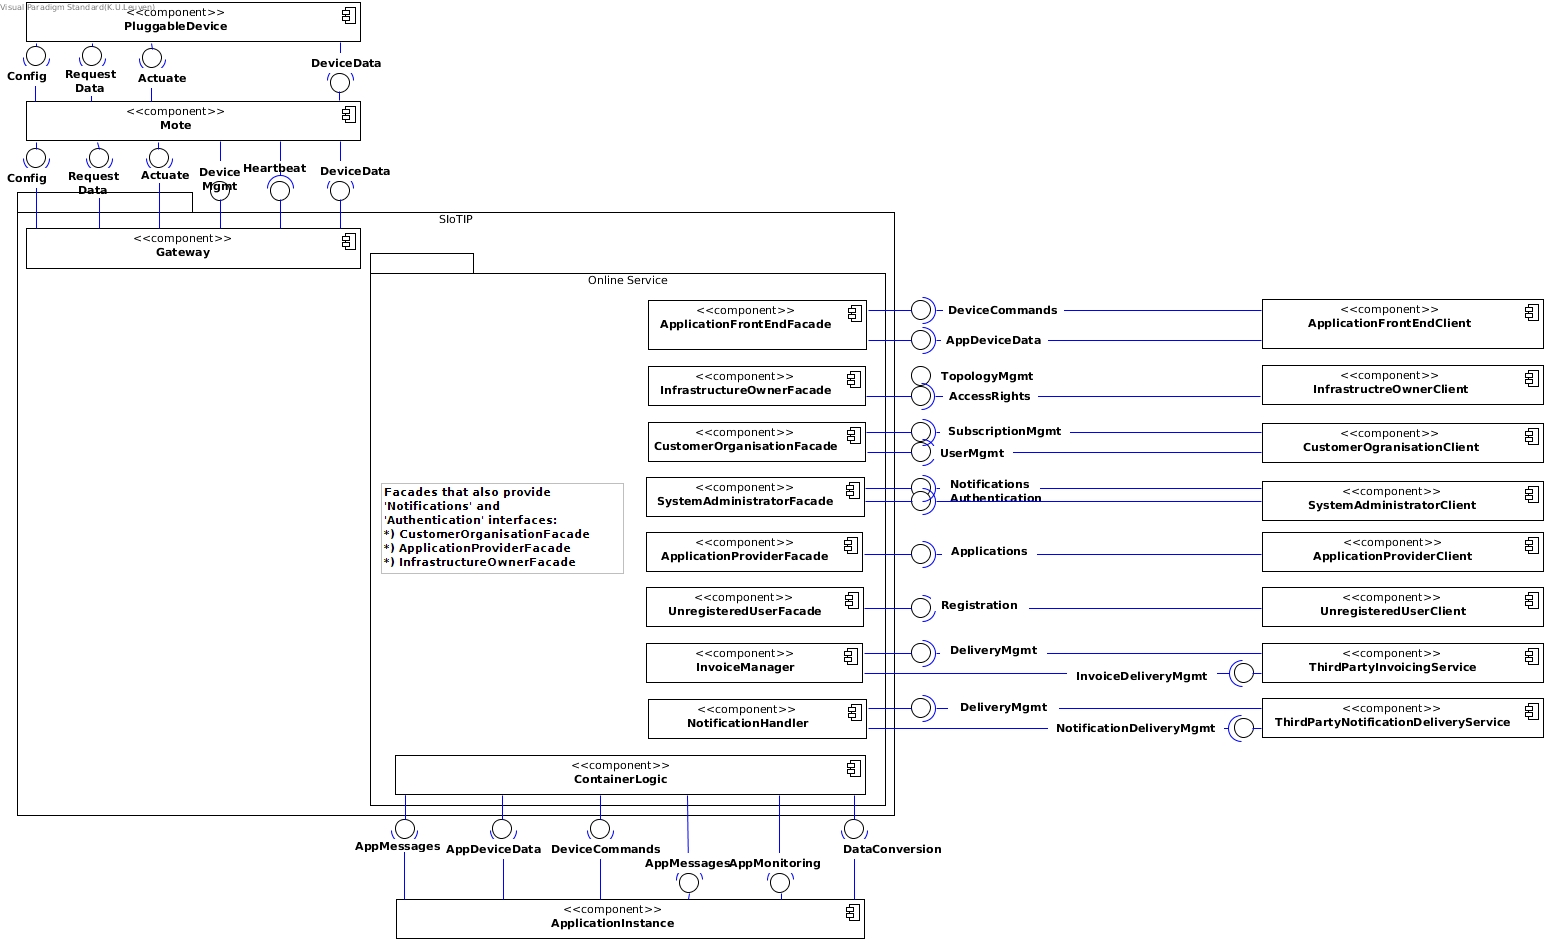
\includegraphics[width=\linewidth]{images/component-CONTEXT}
            \caption{Context diagram for the client-server view.}\label{fig:cc-context}
        \end{figure}

        \vfill
    \end{landscape}

\section{Primary diagram}
    The primary diagram of the client-server view is displayed in figure \ref{fig:cc-primary}. \\

    \todoinline{The primary diagram and accompanying explanation.}

    \begin{landscape}
        \centering
        \vspace*{\fill}

        \begin{figure}[!htp]
            \centering
            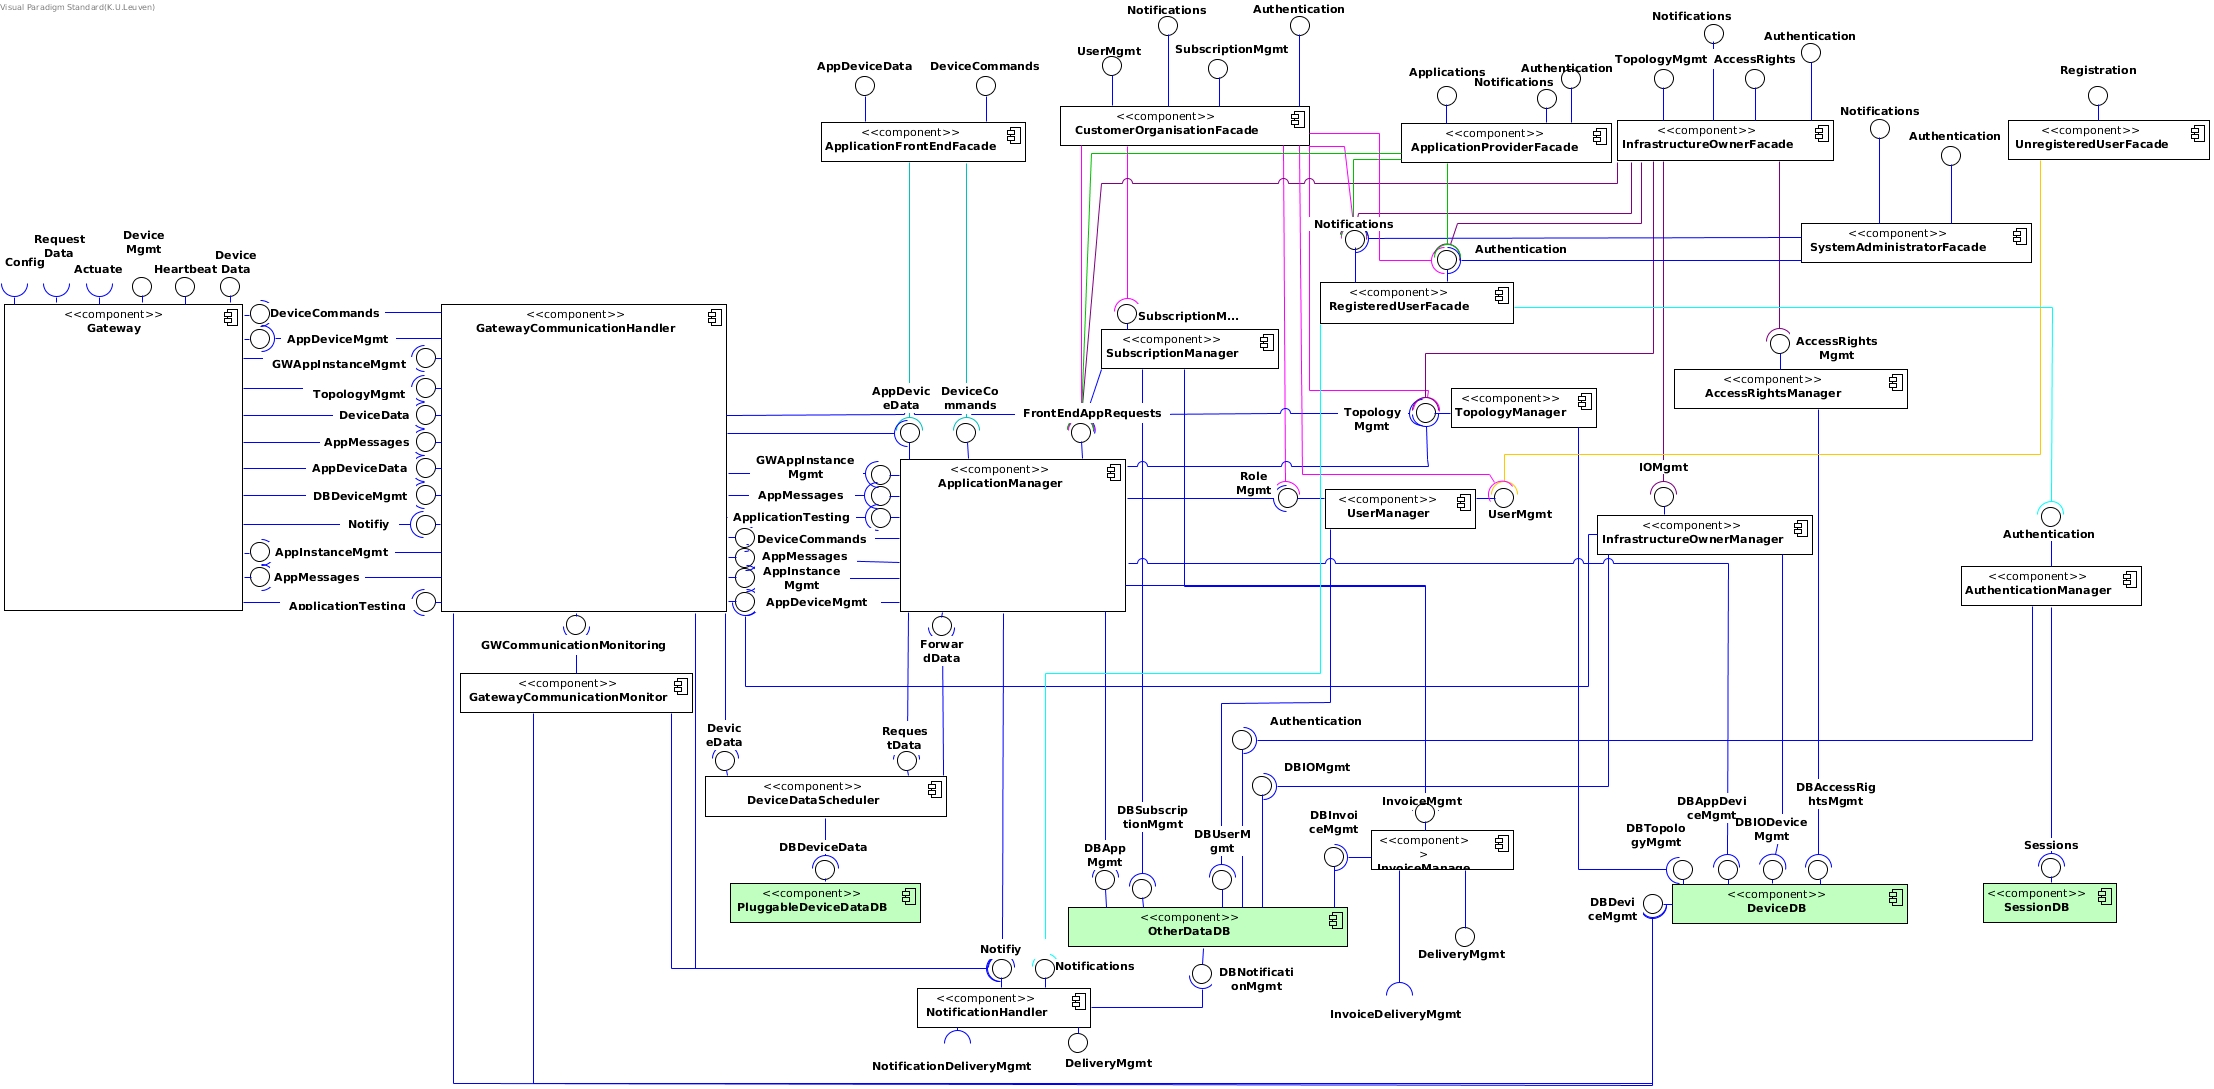
\includegraphics[width=\linewidth]{images/component-PRIMARY}
            \caption{Primary diagram of the client-server view.}\label{fig:cc-primary}
        \end{figure}

        \vfill
    \end{landscape}

    \clearpage

\chapter{Decomposition view (UML Component diagram)}\label{ch:decomposition}
    \minilof
    %\chapter{Decomposition view (UML Component diagram)}\label{ch:decomposition}

% Delete the command below to remove the hints and instructions
\showdecompnotes{}

\begin{figure}[!htp]
	\centering
	%\includegraphics[width=\textwidth]{}
	\missingfigure[figwidth=0.8\textwidth]{Diagram showing decomposition of ComponentX}
	\caption{Decomposition of \texttt{ComponentX}}\label{fig:decomp-componentx}
\end{figure}

\begin{figure}[!htp]
	\centering
	%\includegraphics[width=\textwidth]{}
	\missingfigure[figwidth=0.8\textwidth]{Diagram showing decomposition of ComponentX}
	\caption[Decomposition of \texttt{ComponentY}]{Decomposition of \texttt{ComponentY}.\\
	This caption contains a longer explanation over multiple lines. This additional explanation is not shown in the list of figures.}\label{fig:decomp-componenty}
\end{figure}

    \clearpage
    % \stoplist[decomp]{lof}

\chapter{Deployment view (UML Deployment diagram)}\label{ch:deployment}
    \minilof
    % \chapter{Deployment view (UML Deployment diagram)}\label{ch:deployment}


\begin{landscape}
    \section{Context diagram}
    The context diagram for the deployment view is displayed in figure \ref{fig:depl_context}. \\

    \centering
    \vspace*{\fill}

        \begin{figure}[!htp]
        	\centering
            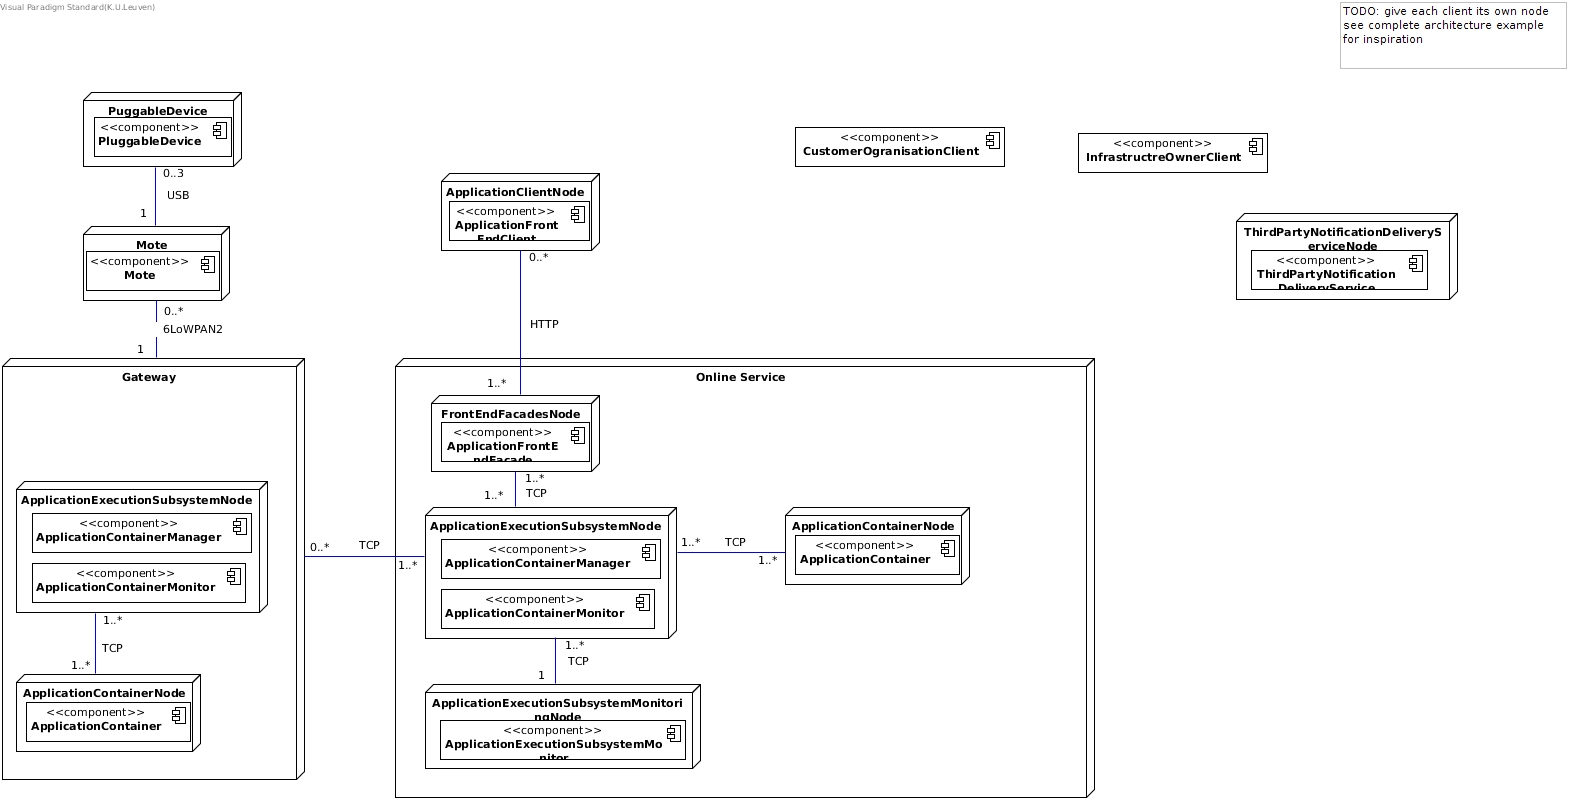
\includegraphics[width=\textwidth]{images/deployment-context}
            \caption{Context diagram for the deployment view.}\label{fig:depl_context}
        \end{figure}

    \vfill
\end{landscape}


\begin{landscape}
    \section{Primary diagram}
    The primary diagram for the deployment view is displayed in figure \ref{fig:depl_primary}.

    \centering
    \vspace*{\fill}

        \begin{figure}[!htp]
        	\centering
            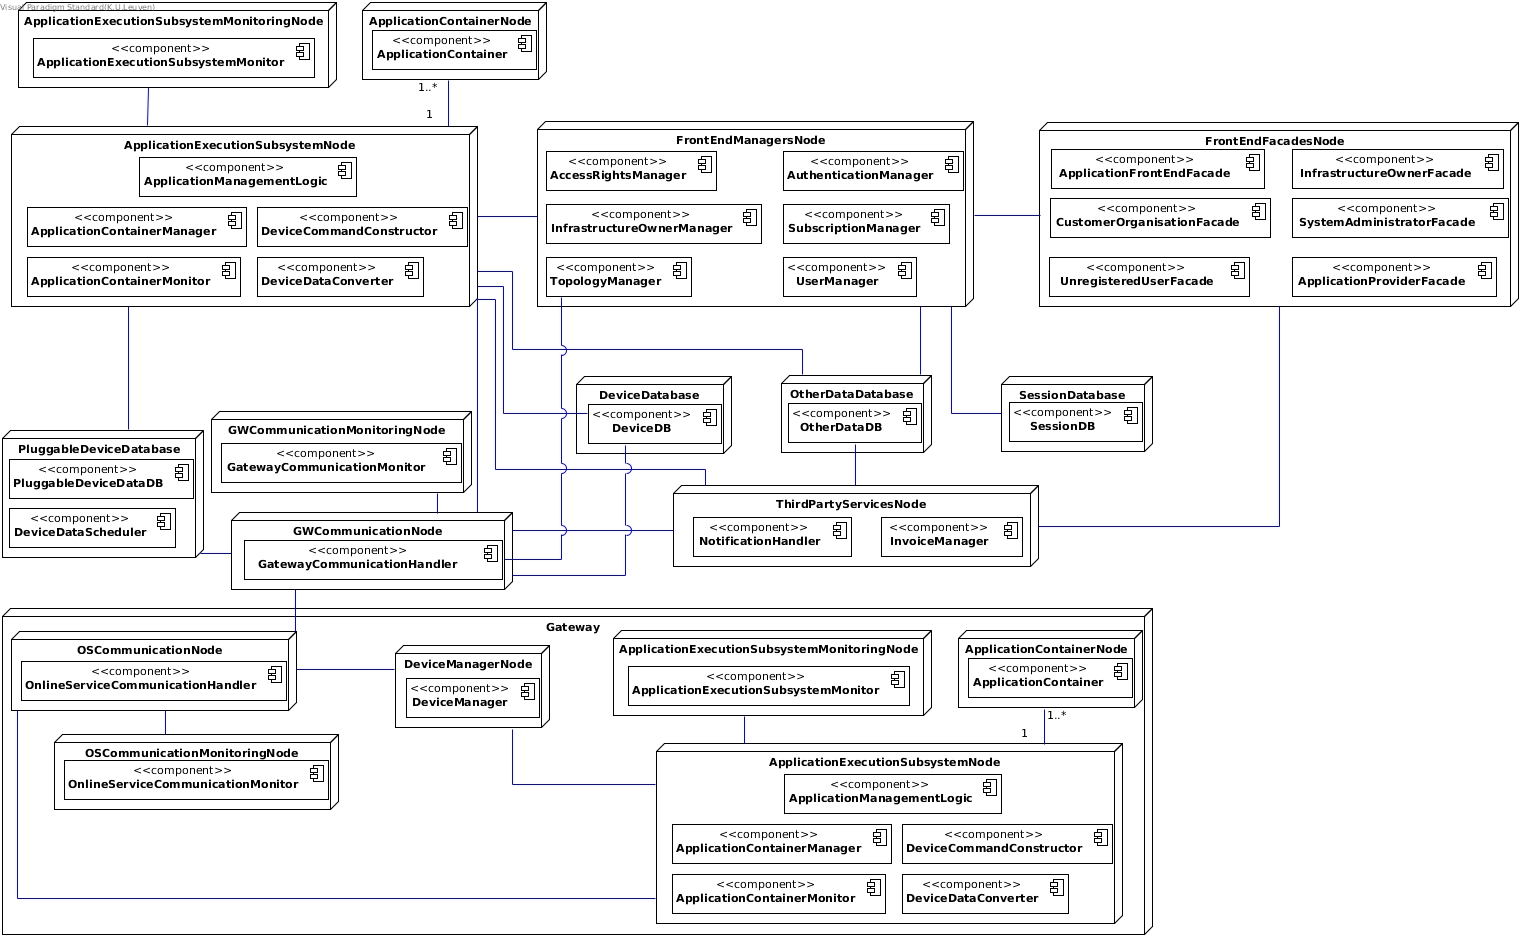
\includegraphics[width=\textwidth]{images/deployment-primary}
        	\caption{Primary diagram for the deployment view.}\label{fig:depl_primary}
        \end{figure}

    \vfill
\end{landscape}

    \clearpage

\chapter{Scenarios}\label{ch:scenarios}
    \minilof
    % \chapter{Scenarios}\label{ch:scenarios}

% Delete the command below to remove the hints and instructions
\showscenariosnotes{}

\todoinline{
	Illustrate how your architecture fulfills the most important data flows. As a rule of thumb, focus on the scenario of the assignment. Describe the scenario in terms of architectural components using UML Sequence diagrams and further explain the most important interactions in text. Illustrating the scenarios serves as a quick validation of the completeness of
	your architecture. If you notice at this point that for some reason, certain functionality or qualities are not addressed sufficiently in your architecture, it suffices to
	document this, together with a rationale of why this is the case according to you. You do not have to further refine you architecture at this point.}


\begin{figure}[!htp]
	\centering
	%\includegraphics[width=\textwidth]{}
	\missingfigure[figwidth=0.8\textwidth]{Sequence diagram scenario 1}
	\caption[Scenario 1]{The system behavior for the first scenario.}\label{fig:seq_scenario1}
\end{figure}


% TODO: before submitting report, replace the chapter line in "exported_catalog.tex" by this line and generate the report 2 times to set all references
% TODO: before submitting report, add \newpage before \section{Interfaces} in "exported_catalog.tex"
\chapter{Element Catalog and Datatypes}\label{ch:elements-datatypes}
    % TODO: before submitting report, move this into exported_catalog
    Each method contains a short note on why the method was added (under "Created for").
    This was done to keep track of our decisions and does not mean that the methods can only
    be used for the Quality Attribute/Use Case referenced in the "Created for" note.
%%% element catalog, generated on Tue May 02 13:13:41 CEST 2017

%%%%
%% The following is a minimal header that allows you to compile a 'standalone' version of the catalog.
%% Uncomment these lines and dont forget to uncomment the \end{document} at the bottom.
%%%%
%% START MINIMAL HEADER
%\documentclass[a4paper,10pt]{report}
%% this package is not strictly needed
%\usepackage[top=2cm,bottom=2cm,left=2cm,right=2cm]{geometry}
%% the following packages are necessary
%\usepackage{enumitem}
%\usepackage{tikz}
%\usepackage{nameref}
%\usepackage{hyperref}
%
%\begin{document}
%% END MINIMAL HEADER


% EXPORT CMDS
% \texttt layout modifications

\newcommand*\vpejustify{%
	\fontdimen2\font=0.4em%
	\fontdimen3\font=0.8em%
	\fontdimen4\font=0.1em%
	\fontdimen7\font=1.0em%
	\hyphenchar\font=`\-\relax%
}
\newcommand{\vpett}[1]{\vpejustify{\texttt{#1}}}

% item labels
\makeatletter
\def\vpeitemlabel#1#2{\begingroup
	#2%
	\def\@currentlabel{#2}%
	\phantomsection\label{#1}\endgroup
}
\makeatother

% vpe operation
\newcommand{\vpeoperation}[1]{#1}

% vpe data type
\newcommand{\vpedatatype}[2]{\vpeitemlabel{#1}{\textbf{\textsf{#2}}}}

% vpe exception
\newcommand{\vpeexception}[2]{\vpeitemlabel{#1}{\textsl{#2}}}



\newcommand{\iconcomponent}{%
	\begin{tikzpicture}[scale=0.3,thin,baseline=-0.5ex]
	\draw (0,0) rectangle (0.4, 0.6);
	\draw [fill=white] (-0.1,0.40) rectangle +(0.25, 0.1);
	\draw [fill=white] (-0.1,0.22) rectangle +(0.25, 0.1);	
	\end{tikzpicture}%
}
\newcommand{\iconprovided}{%
	\begin{tikzpicture}[scale=0.25,thin,baseline=-0.5ex]
	\draw (0.60,0.25) circle [radius=0.25];
	\draw (0, 0.25) -- (0.35, 0.25);
	\end{tikzpicture}%
}
\newcommand{\iconrequired}{%
	\begin{tikzpicture}[scale=0.25,thin,baseline=-0.5ex]
	\draw (0.60,0) arc (270:90:0.25);
	\draw (0, 0.25) -- (0.35, 0.25);
	\end{tikzpicture}%
}
%  END EXPORT CMDS

\chapter{Catalog}
% COMPONENTS
\section{Components}\label{sec:components}
\subsection{AccessRightsManager}\label{comp:OnlineServiceOnlineServiceAccessRightsManager}
	\begin{description}[noitemsep,nolistsep]
		\item[Responsibility:]~Responsible for all functionality related to access rights to pluggable devices.
E.g. retrieving the access rights a customer organisation has for a device,
updating access rights for customer organisations, etc.
		\item[Super-components:]~None
		\item[Sub-components:]~None
		\item[Provided interfaces:]~\iconprovided{}~\vpett{\nameref{int:OnlineServiceOnlineServiceAccessRightsManagerAccessRightsMgmt}}
		\item[Required interfaces:]~\iconrequired{}~\vpett{\nameref{int:DeviceDatabaseDeviceDBAccessRightsMgmt}}		
	\end{description}
\subsection{ActuationCommandConstructor}\label{comp:OnlineServiceOnlineServiceApplicationManagerActuationCommandConstructor}
	\begin{description}[noitemsep,nolistsep]
		\item[Responsibility:]~{\colorbox{red!30}{\underline{Undefined}}}
		\item[Super-components:]~\iconcomponent{}~\vpett{\nameref{comp:OnlineServiceOnlineServiceApplicationManager}}
		\item[Sub-components:]~None
		\item[Provided interfaces:]~\iconprovided{}~\vpett{\nameref{int:OnlineServiceOnlineServiceApplicationManagerActuation}}
		\item[Required interfaces:]~\iconrequired{}~\vpett{\nameref{int:GatewayGatewayAppDeviceMgmt}}		
	\end{description}
\subsection{ApplicationClient}\label{comp:ApplicationClient}
	\begin{description}[noitemsep,nolistsep]
		\item[Responsibility:]~{\colorbox{red!30}{\underline{Undefined}}}
		\item[Super-components:]~None
		\item[Sub-components:]~None
		\item[Provided interfaces:]~None
		\item[Required interfaces:]~\iconrequired{}~\vpett{\nameref{int:OnlineServiceOnlineServiceApplicationFacadeAppData}}, \iconrequired{}~\vpett{\nameref{int:OnlineServiceOnlineServiceApplicationFacadeDeviceMgmt}}, \iconrequired{}~\vpett{\nameref{int:OnlineServiceOnlineServiceApplicationFacadeTopologyOverview}}		
	\end{description}
\subsection{ApplicationContainer}\label{comp:OnlineServiceOnlineServiceApplicationManagerApplicationContainer}
	\begin{description}[noitemsep,nolistsep]
		\item[Responsibility:]~This component contains sanbox environments for application instances to execute in.
		\item[Super-components:]~\iconcomponent{}~\vpett{\nameref{comp:OnlineServiceOnlineServiceApplicationManager}}
		\item[Sub-components:]~None
		\item[Provided interfaces:]~\iconprovided{}~\vpett{\nameref{int:OnlineServiceOnlineServiceApplicationManagerAppInstanceMgmt}}
		\item[Required interfaces:]~None		
	\end{description}
\subsection{ApplicationContainerManager}\label{comp:OnlineServiceOnlineServiceApplicationManagerApplicationContainerManager}
	\begin{description}[noitemsep,nolistsep]
		\item[Responsibility:]~This component contains sanbox environments for application instances to execute in.
		\item[Super-components:]~\iconcomponent{}~\vpett{\nameref{comp:OnlineServiceOnlineServiceApplicationManager}}
		\item[Sub-components:]~None
		\item[Provided interfaces:]~\iconprovided{}~\vpett{\nameref{int:OnlineServiceOnlineServiceApplicationManagerApps}}
		\item[Required interfaces:]~\iconrequired{}~\vpett{\nameref{int:OnlineServiceOnlineServiceApplicationManagerAppInstanceMgmt}}		
	\end{description}
\subsection{ApplicationContainerMonitor}\label{comp:OnlineServiceOnlineServiceApplicationManagerApplicationContainerMonitor}
	\begin{description}[noitemsep,nolistsep]
		\item[Responsibility:]~{\colorbox{red!30}{\underline{Undefined}}}
		\item[Super-components:]~\iconcomponent{}~\vpett{\nameref{comp:OnlineServiceOnlineServiceApplicationManager}}
		\item[Sub-components:]~None
		\item[Provided interfaces:]~None
		\item[Required interfaces:]~\iconrequired{}~\vpett{\nameref{int:OnlineServiceOnlineServiceApplicationManagerAppInstanceMgmt}}		
	\end{description}
\subsection{ApplicationFacade}\label{comp:OnlineServiceOnlineServiceApplicationFacade}
	\begin{description}[noitemsep,nolistsep]
		\item[Responsibility:]~{\colorbox{red!30}{\underline{Undefined}}}
		\item[Super-components:]~None
		\item[Sub-components:]~None
		\item[Provided interfaces:]~\iconprovided{}~\vpett{\nameref{int:OnlineServiceOnlineServiceApplicationFacadeAppData}}, \iconprovided{}~\vpett{\nameref{int:OnlineServiceOnlineServiceApplicationFacadeDeviceMgmt}}, \iconprovided{}~\vpett{\nameref{int:OnlineServiceOnlineServiceApplicationFacadeTopologyOverview}}
		\item[Required interfaces:]~\iconrequired{}~\vpett{\nameref{int:OnlineServiceOnlineServiceApplicationManagerActuation}}, \iconrequired{}~\vpett{\nameref{int:OnlineServiceOnlineServiceApplicationManagerApps}}		
	\end{description}
\subsection{ApplicationLogic}\label{comp:OnlineServiceOnlineServiceApplicationManagerApplicationLogic}
	\begin{description}[noitemsep,nolistsep]
		\item[Responsibility:]~{\colorbox{red!30}{\underline{Undefined}}}
		\item[Super-components:]~\iconcomponent{}~\vpett{\nameref{comp:OnlineServiceOnlineServiceApplicationManager}}
		\item[Sub-components:]~None
		\item[Provided interfaces:]~None
		\item[Required interfaces:]~None		
	\end{description}
\subsection{ApplicationManager}\label{comp:OnlineServiceOnlineServiceApplicationManager}
	\begin{description}[noitemsep,nolistsep]
		\item[Responsibility:]~Responsible for activating/deactivating applications, setting pluggable device redundancy requirements on \vpett{\nameref{comp:GatewayGatewayDeviceManager}} components, and using \vpett{\nameref{comp:OnlineServiceOnlineServiceNotificationHandler}} to send notifications to customer organisations.
		\item[Super-components:]~None
		\item[Sub-components:]~\iconcomponent{}~\vpett{\nameref{comp:OnlineServiceOnlineServiceApplicationManagerActuationCommandConstructor}}, \iconcomponent{}~\vpett{\nameref{comp:OnlineServiceOnlineServiceApplicationManagerApplicationContainerMonitor}}, \iconcomponent{}~\vpett{\nameref{comp:OnlineServiceOnlineServiceApplicationManagerApplicationContainer}}, \iconcomponent{}~\vpett{\nameref{comp:OnlineServiceOnlineServiceApplicationManagerApplicationContainerManager}}, \iconcomponent{}~\vpett{\nameref{comp:OnlineServiceOnlineServiceApplicationManagerApplicationLogic}}
		\item[Provided interfaces:]~\iconprovided{}~\vpett{\nameref{int:OnlineServiceOnlineServiceApplicationManagerActuation}}, \iconprovided{}~\vpett{\nameref{int:OnlineServiceOnlineServiceApplicationManagerAppMgmt}}, \iconprovided{}~\vpett{\nameref{int:OnlineServiceOnlineServiceApplicationManagerApps}}, \iconprovided{}~\vpett{\nameref{int:OnlineServiceOnlineServiceApplicationManagerForwardData}}, \iconprovided{}~\vpett{\nameref{int:OnlineServiceOnlineServiceApplicationManagerIOAppMgmt}}
		\item[Required interfaces:]~\iconrequired{}~\vpett{\nameref{int:GatewayGatewayAppDeviceMgmt}}, \iconrequired{}~\vpett{\nameref{int:OtherDataDatabaseOtherDataDBAppMgmt}}, \iconrequired{}~\vpett{\nameref{int:GatewayGatewayGWApplicationContainerManagerAppMgmt}}, \iconrequired{}~\vpett{\nameref{int:OnlineServiceOnlineServiceInvoiceManagerInvoiceMgmt}}, \iconrequired{}~\vpett{\nameref{int:OnlineServiceOnlineServiceNotificationHandlerNotify}}, \iconrequired{}~\vpett{\nameref{int:OnlineServiceOnlineServiceDeviceDataSchedulerRequestData}}, \iconrequired{}~\vpett{\nameref{int:OnlineServiceOnlineServiceUserRolesManagerRoleMgmt}}, \iconrequired{}~\vpett{\nameref{int:OnlineServiceOnlineServiceTopologyManagerTopologyMgmt}}		
	\end{description}
\subsection{CustomerOgranisationClient}\label{comp:CustomerOgranisationClient}
	\begin{description}[noitemsep,nolistsep]
		\item[Responsibility:]~Represents the client used by a customer organisation. This is the user's dashboard.
		\item[Super-components:]~None
		\item[Sub-components:]~None
		\item[Provided interfaces:]~None
		\item[Required interfaces:]~\iconrequired{}~\vpett{\nameref{int:OnlineServiceOnlineServiceCustomerOrganisationFacadeSubscriptionMgmt}}		
	\end{description}
\subsection{CustomerOrganisationFacade}\label{comp:OnlineServiceOnlineServiceCustomerOrganisationFacade}
	\begin{description}[noitemsep,nolistsep]
		\item[Responsibility:]~Acts as an access point for CustomerOrganisationClients and handles all functionality that can be done by customer organisations.
		\item[Super-components:]~None
		\item[Sub-components:]~None
		\item[Provided interfaces:]~\iconprovided{}~\vpett{\nameref{int:OnlineServiceOnlineServiceCustomerOrganisationFacadeSubscriptionMgmt}}
		\item[Required interfaces:]~\iconrequired{}~\vpett{\nameref{int:OnlineServiceOnlineServiceApplicationManagerApps}}, \iconrequired{}~\vpett{\nameref{int:OnlineServiceOnlineServiceUserRolesManagerRoleMgmt}}, \iconrequired{}~\vpett{\nameref{int:OnlineServiceOnlineServiceSubscriptionManagerSubscriptionMgmt}}, \iconrequired{}~\vpett{\nameref{int:OnlineServiceOnlineServiceTopologyManagerTopologyMgmt}}		
	\end{description}
\subsection{DeviceDataConverter}\label{comp:OnlineServiceOnlineServiceDeviceDataConverter}
	\begin{description}[noitemsep,nolistsep]
		\item[Responsibility:]~The \vpett{\nameref{comp:OnlineServiceOnlineServiceDeviceDataConverter}} is resposible for converting pluggable device data in the data processing subsystem.
		\item[Super-components:]~None
		\item[Sub-components:]~None
		\item[Provided interfaces:]~\iconprovided{}~\vpett{\nameref{int:OnlineServiceOnlineServiceDeviceDataConverterDataConversion}}
		\item[Required interfaces:]~None		
	\end{description}
\subsection{DeviceDataScheduler}\label{comp:OnlineServiceOnlineServiceDeviceDataScheduler}
	\begin{description}[noitemsep,nolistsep]
		\item[Responsibility:]~Responsible for scheduling incoming read and write requests for pluggable device data. Monitors throughput of requests and switches between normal and overload mode when appropriate. Avoids starvation of any type of request.
		\item[Super-components:]~None
		\item[Sub-components:]~None
		\item[Provided interfaces:]~\iconprovided{}~\vpett{\nameref{int:OnlineServiceOnlineServiceDeviceDataSchedulerDeviceData}}, \iconprovided{}~\vpett{\nameref{int:OnlineServiceOnlineServiceDeviceDataSchedulerRequestData}}
		\item[Required interfaces:]~\iconrequired{}~\vpett{\nameref{int:PluggableDeviceDatabasePluggableDeviceDataDBDeviceData}}, \iconrequired{}~\vpett{\nameref{int:OnlineServiceOnlineServiceApplicationManagerForwardData}}		
	\end{description}
\subsection{DeviceDB}\label{comp:DeviceDatabaseDeviceDB}
	\begin{description}[noitemsep,nolistsep]
		\item[Responsibility:]~Contains all information related to devices in the system, but not pluggable device data such as sensor data or actuation statuses. The data includes information about pluggable devices, motes, gateways, topologies, access rights, etc.
		\item[Super-components:]~None
		\item[Sub-components:]~None
		\item[Provided interfaces:]~\iconprovided{}~\vpett{\nameref{int:DeviceDatabaseDeviceDBAccessRightsMgmt}}, \iconprovided{}~\vpett{\nameref{int:DeviceDatabaseDeviceDBDeviceMgmt}}, \iconprovided{}~\vpett{\nameref{int:DeviceDatabaseDeviceDBIODeviceMgmt}}, \iconprovided{}~\vpett{\nameref{int:DeviceDatabaseDeviceDBTopologyMgmt}}
		\item[Required interfaces:]~None		
	\end{description}
\subsection{DeviceManager}\label{comp:GatewayGatewayDeviceManager}
	\begin{description}[noitemsep,nolistsep]
		\item[Responsibility:]~Monitors connected/operational devices on a gateway. Sends notifications in case of hardware failure. Can send a command to disable or reactivate applications when necessary.
		\item[Super-components:]~\iconcomponent{}~\vpett{\nameref{comp:GatewayGateway}}
		\item[Sub-components:]~None
		\item[Provided interfaces:]~\iconprovided{}~\vpett{\nameref{int:GatewayGatewayDeviceManagerDeviceMgmt}}
		\item[Required interfaces:]~\iconrequired{}~\vpett{\nameref{int:GatewayGatewayDeviceMgmt}}		
	\end{description}
\subsection{Gateway}\label{comp:GatewayGateway}
	\begin{description}[noitemsep,nolistsep]
		\item[Responsibility:]~Main component on the gateway that allows different components to work
with each other. E.g. transmits heartbeats from motes to
\vpett{\nameref{comp:GatewayGatewayDeviceManager}}, transmits commands to shut down applications,
triggers notifications to be generated, ...
		\item[Super-components:]~None
		\item[Sub-components:]~\iconcomponent{}~\vpett{\nameref{comp:GatewayGatewayGatewayLogic}}, \iconcomponent{}~\vpett{\nameref{comp:GatewayGatewayDeviceManager}}, \iconcomponent{}~\vpett{\nameref{comp:GatewayGatewayGWApplicationContainerManager}}
		\item[Provided interfaces:]~\iconprovided{}~\vpett{\nameref{int:GatewayGatewayAppDeviceMgmt}}, \iconprovided{}~\vpett{\nameref{int:GatewayGatewayGWApplicationContainerManagerAppMgmt}}, \iconprovided{}~\vpett{\nameref{int:GatewayGatewayDeviceData}}, \iconprovided{}~\vpett{\nameref{int:GatewayGatewayDeviceMgmt}}, \iconprovided{}~\vpett{\nameref{int:GatewayGatewayHeartbeat}}
		\item[Required interfaces:]~\iconrequired{}~\vpett{\nameref{int:OnlineServiceOnlineServiceApplicationManagerAppMgmt}}, \iconrequired{}~\vpett{\nameref{int:OnlineServiceOnlineServiceDeviceDataConverterDataConversion}}, \iconrequired{}~\vpett{\nameref{int:OnlineServiceOnlineServiceDeviceDataSchedulerDeviceData}}, \iconrequired{}~\vpett{\nameref{int:MoteMoteDeviceMgmt}}, \iconrequired{}~\vpett{\nameref{int:GatewayGatewayDeviceManagerDeviceMgmt}}, \iconrequired{}~\vpett{\nameref{int:DeviceDatabaseDeviceDBDeviceMgmt}}, \iconrequired{}~\vpett{\nameref{int:OnlineServiceOnlineServiceNotificationHandlerNotify}}, \iconrequired{}~\vpett{\nameref{int:OnlineServiceOnlineServiceTopologyManagerTopologyMgmt}}		
	\end{description}
\subsection{GatewayLogic}\label{comp:GatewayGatewayGatewayLogic}
	\begin{description}[noitemsep,nolistsep]
		\item[Responsibility:]~Handles the main logic on the gateway and communication with other outside components.
		\item[Super-components:]~\iconcomponent{}~\vpett{\nameref{comp:GatewayGateway}}
		\item[Sub-components:]~None
		\item[Provided interfaces:]~\iconprovided{}~\vpett{\nameref{int:GatewayGatewayAppDeviceMgmt}}, \iconprovided{}~\vpett{\nameref{int:GatewayGatewayDeviceData}}, \iconprovided{}~\vpett{\nameref{int:GatewayGatewayDeviceMgmt}}, \iconprovided{}~\vpett{\nameref{int:GatewayGatewayHeartbeat}}
		\item[Required interfaces:]~\iconrequired{}~\vpett{\nameref{int:OnlineServiceOnlineServiceApplicationManagerAppMgmt}}, \iconrequired{}~\vpett{\nameref{int:GatewayGatewayClass}}, \iconrequired{}~\vpett{\nameref{int:GatewayGatewayDeviceManagerDeviceMgmt}}, \iconrequired{}~\vpett{\nameref{int:MoteMoteDeviceMgmt}}		
	\end{description}
\subsection{GWApplicationContainerManager}\label{comp:GatewayGatewayGWApplicationContainerManager}
	\begin{description}[noitemsep,nolistsep]
		\item[Responsibility:]~{\colorbox{red!30}{\underline{Undefined}}}
		\item[Super-components:]~\iconcomponent{}~\vpett{\nameref{comp:GatewayGateway}}
		\item[Sub-components:]~None
		\item[Provided interfaces:]~\iconprovided{}~\vpett{\nameref{int:GatewayGatewayGWApplicationContainerManagerAppMgmt}}
		\item[Required interfaces:]~None		
	\end{description}
\subsection{InfrastructreOwnerClient}\label{comp:InfrastructreOwnerClient}
	\begin{description}[noitemsep,nolistsep]
		\item[Responsibility:]~Represents the client used by an infrastructure owner. This is the user's dashboard.
		\item[Super-components:]~None
		\item[Sub-components:]~None
		\item[Provided interfaces:]~None
		\item[Required interfaces:]~\iconrequired{}~\vpett{\nameref{int:OnlineServiceOnlineServiceInfrastructureOwnerFacadeAccessRights}}		
	\end{description}
\subsection{InfrastructureOwnerFacade}\label{comp:OnlineServiceOnlineServiceInfrastructureOwnerFacade}
	\begin{description}[noitemsep,nolistsep]
		\item[Responsibility:]~Acts as an access point for InfrastructureOwnerClients and handles all functionality that can be done by infrastructure owners.
		\item[Super-components:]~None
		\item[Sub-components:]~None
		\item[Provided interfaces:]~\iconprovided{}~\vpett{\nameref{int:OnlineServiceOnlineServiceInfrastructureOwnerFacadeAccessRights}}
		\item[Required interfaces:]~\iconrequired{}~\vpett{\nameref{int:OnlineServiceOnlineServiceAccessRightsManagerAccessRightsMgmt}}, \iconrequired{}~\vpett{\nameref{int:OnlineServiceOnlineServiceApplicationManagerIOAppMgmt}}, \iconrequired{}~\vpett{\nameref{int:OnlineServiceOnlineServiceInfrastructureOwnerManagerIOMgmt}}		
	\end{description}
\subsection{InfrastructureOwnerManager}\label{comp:OnlineServiceOnlineServiceInfrastructureOwnerManager}
	\begin{description}[noitemsep,nolistsep]
		\item[Responsibility:]~Responsible for all functionality related to infrastructure owners. E.g. looking up the devices they own, retrieving a list of customer organisations that they are associated to, etc.
		\item[Super-components:]~None
		\item[Sub-components:]~None
		\item[Provided interfaces:]~\iconprovided{}~\vpett{\nameref{int:OnlineServiceOnlineServiceInfrastructureOwnerManagerIOMgmt}}
		\item[Required interfaces:]~\iconrequired{}~\vpett{\nameref{int:DeviceDatabaseDeviceDBIODeviceMgmt}}, \iconrequired{}~\vpett{\nameref{int:OtherDataDatabaseOtherDataDBIOMgmt}}		
	\end{description}
\subsection{InvoiceManager}\label{comp:OnlineServiceOnlineServiceInvoiceManager}
	\begin{description}[noitemsep,nolistsep]
		\item[Responsibility:]~Responsible for all functionality related to access rights to invoicing.
E.g. creating invoices.
		\item[Super-components:]~None
		\item[Sub-components:]~None
		\item[Provided interfaces:]~\iconprovided{}~\vpett{\nameref{int:OnlineServiceOnlineServiceInvoiceManagerInvoiceMgmt}}
		\item[Required interfaces:]~\iconrequired{}~\vpett{\nameref{int:OtherDataDatabaseOtherDataDBInvoiceMgmt}}		
	\end{description}
\subsection{Mote}\label{comp:MoteMote}
	\begin{description}[noitemsep,nolistsep]
		\item[Responsibility:]~Sends heartbeats to the GatewayFacade. Includes a list
of connected pluggable devices in the heartbeats.
		\item[Super-components:]~None
		\item[Sub-components:]~None
		\item[Provided interfaces:]~\iconprovided{}~\vpett{\nameref{int:MoteMoteDeviceData}}, \iconprovided{}~\vpett{\nameref{int:MoteMoteDeviceMgmt}}
		\item[Required interfaces:]~\iconrequired{}~\vpett{\nameref{int:PuggableDevicePluggableDeviceActuate}}, \iconrequired{}~\vpett{\nameref{int:PuggableDevicePluggableDeviceConfig}}, \iconrequired{}~\vpett{\nameref{int:GatewayGatewayDeviceData}}, \iconrequired{}~\vpett{\nameref{int:GatewayGatewayHeartbeat}}, \iconrequired{}~\vpett{\nameref{int:PuggableDevicePluggableDeviceRequestData}}		
	\end{description}
\subsection{NotificationDeliveryService}\label{comp:NotificationDeliveryServiceNodeNotificationDeliveryService}
	\begin{description}[noitemsep,nolistsep]
		\item[Responsibility:]~{\colorbox{red!30}{\underline{Undefined}}}
		\item[Super-components:]~None
		\item[Sub-components:]~None
		\item[Provided interfaces:]~None
		\item[Required interfaces:]~None		
	\end{description}
\subsection{NotificationHandler}\label{comp:OnlineServiceOnlineServiceNotificationHandler}
	\begin{description}[noitemsep,nolistsep]
		\item[Responsibility:]~Responsible for generation, storage, and delivery of notifications based on users' preferred communication channel.
		\item[Super-components:]~None
		\item[Sub-components:]~None
		\item[Provided interfaces:]~\iconprovided{}~\vpett{\nameref{int:OnlineServiceOnlineServiceNotificationHandlerDeliveryMgmt}}, \iconprovided{}~\vpett{\nameref{int:OnlineServiceOnlineServiceNotificationHandlerNotify}}
		\item[Required interfaces:]~\iconrequired{}~\vpett{\nameref{int:NotificationDeliveryServiceNodeNotificationDeliveryServiceNotificationDeliveryMgmt}}, \iconrequired{}~\vpett{\nameref{int:OtherDataDatabaseOtherDataDBNotificationMgmt}}		
	\end{description}
\subsection{OtherDataDB}\label{comp:OtherDataDatabaseOtherDataDB}
	\begin{description}[noitemsep,nolistsep]
		\item[Responsibility:]~General database for data. For example, storage of data about notifications.
		\item[Super-components:]~None
		\item[Sub-components:]~None
		\item[Provided interfaces:]~\iconprovided{}~\vpett{\nameref{int:OtherDataDatabaseOtherDataDBAppMgmt}}, \iconprovided{}~\vpett{\nameref{int:OtherDataDatabaseOtherDataDBInvoiceMgmt}}, \iconprovided{}~\vpett{\nameref{int:OtherDataDatabaseOtherDataDBIOMgmt}}, \iconprovided{}~\vpett{\nameref{int:OtherDataDatabaseOtherDataDBNotificationMgmt}}, \iconprovided{}~\vpett{\nameref{int:OtherDataDatabaseOtherDataDBSubscriptionMgmt}}, \iconprovided{}~\vpett{\nameref{int:OtherDataDatabaseOtherDataDBUserRoleMgmt}}
		\item[Required interfaces:]~None		
	\end{description}
\subsection{PluggableDeviceDataDB}\label{comp:PluggableDeviceDatabasePluggableDeviceDataDB}
	\begin{description}[noitemsep,nolistsep]
		\item[Responsibility:]~Database dedicated to pluggable device data only.
		\item[Super-components:]~None
		\item[Sub-components:]~None
		\item[Provided interfaces:]~\iconprovided{}~\vpett{\nameref{int:PluggableDeviceDatabasePluggableDeviceDataDBDeviceData}}
		\item[Required interfaces:]~None		
	\end{description}
\subsection{PluggableDevice}\label{comp:PuggableDevicePluggableDevice}
	\begin{description}[noitemsep,nolistsep]
		\item[Responsibility:]~Responsible for sending pluggable device data to \vpett{\nameref{comp:MoteMote}}. Needs to be initialised in order for the data to be used/stored.
		\item[Super-components:]~None
		\item[Sub-components:]~None
		\item[Provided interfaces:]~\iconprovided{}~\vpett{\nameref{int:PuggableDevicePluggableDeviceActuate}}, \iconprovided{}~\vpett{\nameref{int:PuggableDevicePluggableDeviceConfig}}, \iconprovided{}~\vpett{\nameref{int:PuggableDevicePluggableDeviceRequestData}}
		\item[Required interfaces:]~\iconrequired{}~\vpett{\nameref{int:MoteMoteDeviceData}}		
	\end{description}
\subsection{SubscriptionManager}\label{comp:OnlineServiceOnlineServiceSubscriptionManager}
	\begin{description}[noitemsep,nolistsep]
		\item[Responsibility:]~Responsible for all functionality related to access rights to subscriptions. E.g. retrieving the applications that a customer organisation can subscribe to, creating new subscriptions to ApplicationInstances, etc.
		\item[Super-components:]~None
		\item[Sub-components:]~None
		\item[Provided interfaces:]~\iconprovided{}~\vpett{\nameref{int:OnlineServiceOnlineServiceSubscriptionManagerSubscriptionMgmt}}
		\item[Required interfaces:]~\iconrequired{}~\vpett{\nameref{int:OnlineServiceOnlineServiceApplicationManagerApps}}, \iconrequired{}~\vpett{\nameref{int:OtherDataDatabaseOtherDataDBSubscriptionMgmt}}		
	\end{description}
\subsection{TopologyManager}\label{comp:OnlineServiceOnlineServiceTopologyManager}
	\begin{description}[noitemsep,nolistsep]
		\item[Responsibility:]~Responsible for all functionality related to topology. E.g. Adding a new mote to the topology of an infrastructure, checking whether or not all devices used by an application are active in the topology, etc.
		\item[Super-components:]~None
		\item[Sub-components:]~None
		\item[Provided interfaces:]~\iconprovided{}~\vpett{\nameref{int:OnlineServiceOnlineServiceTopologyManagerTopologyMgmt}}
		\item[Required interfaces:]~\iconrequired{}~\vpett{\nameref{int:DeviceDatabaseDeviceDBTopologyMgmt}}		
	\end{description}
\subsection{UserRolesManager}\label{comp:OnlineServiceOnlineServiceUserRolesManager}
	\begin{description}[noitemsep,nolistsep]
		\item[Responsibility:]~Responsible for all functionality related to access rights to user roles. E.g. retrieving the user roles that are mandatory for a certain application, updating the roles assigned to users, etc.
		\item[Super-components:]~None
		\item[Sub-components:]~None
		\item[Provided interfaces:]~\iconprovided{}~\vpett{\nameref{int:OnlineServiceOnlineServiceUserRolesManagerRoleMgmt}}
		\item[Required interfaces:]~\iconrequired{}~\vpett{\nameref{int:OtherDataDatabaseOtherDataDBUserRoleMgmt}}		
	\end{description}

% END COMPONENTS

% INTERFACES
\section{Interfaces} \label{sec:interfaces}
  %%%%%%%% AccessRights
  \subsection{AccessRights}\label{int:OnlineServiceOnlineServiceInfrastructureOwnerFacadeAccessRights}
    \begin{description}[noitemsep,nolistsep]
      \item[Provided by:] \iconcomponent{}~\vpett{\nameref{comp:OnlineServiceOnlineServiceInfrastructureOwnerFacade}}
      \item[Required by:] \iconcomponent{}~\vpett{\nameref{comp:InfrastructreOwnerClient}}
      \item[Operations:] ~
    \begin{itemize}[noitemsep,nolistsep,leftmargin=-.25cm]
      \item \textsf{ configureDevice(\ref{data:DataTypesPluggableDeviceID} pID)}
        \begin{itemize}[noitemsep,nolistsep]
           \item Effect: Returns a map of AccessRights and the IDs of customer organisations that have those AccessRights.
\item Created for: UC9.3 - UC9.4
        \end{itemize}
      \item \textsf{List\textless{}\ref{data:DataTypesPluggableDeviceInfo}\textgreater{} getAccessRights(int infrastructureOwnerID)}
        \begin{itemize}[noitemsep,nolistsep]
           \item Effect: Returns a list of PluggableDeviceInfo to display so an infrastructure owner can select a device to configure access rights.
\item Created for: UC9.1
        \end{itemize}
      \item \textsf{void updateAccessRights()}
        \begin{itemize}[noitemsep,nolistsep]
           \item Effect: Updates the access rights on a certain pluggable device for a group of customer organisations.
\item Created for: UC9.6
        \end{itemize}
    \end{itemize}
    \end{description}

  %%%%%%%% AccessRightsMgmt
  \subsection{AccessRightsMgmt}\label{int:DeviceDatabaseDeviceDBAccessRightsMgmt}
    \begin{description}[noitemsep,nolistsep]
      \item[Provided by:] \iconcomponent{}~\vpett{\nameref{comp:DeviceDatabaseDeviceDB}}
      \item[Required by:] \iconcomponent{}~\vpett{\nameref{comp:OnlineServiceOnlineServiceAccessRightsManager}}
      \item[Operations:] ~
    \begin{itemize}[noitemsep,nolistsep,leftmargin=-.25cm]
      \item \textsf{ getCustomerOrganisationsRights(\ref{data:DataTypesPluggableDeviceID} pID, List\textless{}int\textgreater{} custOrgIDs)}
        \begin{itemize}[noitemsep,nolistsep]
           \item Effect: Returns a map of AccessRights and the IDs of customer organisations that have those AccessRights on a certain pluggable device.
\item Created for: UC9.4
        \end{itemize}
      \item \textsf{void updateAccessRights()}
        \begin{itemize}[noitemsep,nolistsep]
           \item Effect: Updates the access rights on a certain pluggable device for a group of customer organisations.
\item Created for: UC9.7
        \end{itemize}
    \end{itemize}
    \end{description}

  %%%%%%%% AccessRightsMgmt
  \subsection{AccessRightsMgmt}\label{int:OnlineServiceOnlineServiceAccessRightsManagerAccessRightsMgmt}
    \begin{description}[noitemsep,nolistsep]
      \item[Provided by:] \iconcomponent{}~\vpett{\nameref{comp:OnlineServiceOnlineServiceAccessRightsManager}}
      \item[Required by:] \iconcomponent{}~\vpett{\nameref{comp:OnlineServiceOnlineServiceInfrastructureOwnerFacade}}
      \item[Operations:] ~
    \begin{itemize}[noitemsep,nolistsep,leftmargin=-.25cm]
      \item \textsf{ getCustomerOrganisationsRights(\ref{data:DataTypesPluggableDeviceID} pID, List\textless{}int\textgreater{} custOrgIDs)}
        \begin{itemize}[noitemsep,nolistsep]
           \item Effect: Returns a map of AccessRights and the IDs of customer organisations that have those AccessRights on a certain pluggable device.
\item Created for: UC9.4
        \end{itemize}
      \item \textsf{void updateAccessRights()}
        \begin{itemize}[noitemsep,nolistsep]
           \item Effect: Updates the access rights on a certain pluggable device for a group of customer organisations.
\item Created for: UC9.7
        \end{itemize}
    \end{itemize}
    \end{description}

  %%%%%%%% Actuate
  \subsection{Actuate}\label{int:PuggableDevicePluggableDeviceActuate}
    \begin{description}[noitemsep,nolistsep]
      \item[Provided by:] \iconcomponent{}~\vpett{\nameref{comp:PuggableDevicePluggableDevice}}
      \item[Required by:] \iconcomponent{}~\vpett{\nameref{comp:MoteMote}}
      \item[Operations:] ~
    \begin{itemize}[noitemsep,nolistsep,leftmargin=-.25cm]
      \item \textsf{void sendActuationCommand(string commandName)}
        \begin{itemize}[noitemsep,nolistsep]
           \item Effect: Send an actuation command to the actuator. Sending an unknown actuation command has no effect.
        \end{itemize}
    \end{itemize}
    \end{description}

  %%%%%%%% Actuation
  \subsection{Actuation}\label{int:OnlineServiceOnlineServiceApplicationManagerActuation}
    \begin{description}[noitemsep,nolistsep]
      \item[Provided by:] \iconcomponent{}~\vpett{\nameref{comp:OnlineServiceOnlineServiceApplicationManagerActuationCommandConstructor}}, \iconcomponent{}~\vpett{\nameref{comp:OnlineServiceOnlineServiceApplicationManager}}
      \item[Required by:] \iconcomponent{}~\vpett{\nameref{comp:OnlineServiceOnlineServiceApplicationFacade}}
      \item[Operations:] ~
% no operations
    \end{description}

  %%%%%%%% AppData
  \subsection{AppData}\label{int:OnlineServiceOnlineServiceApplicationFacadeAppData}
    \begin{description}[noitemsep,nolistsep]
      \item[Provided by:] \iconcomponent{}~\vpett{\nameref{comp:OnlineServiceOnlineServiceApplicationFacade}}
      \item[Required by:] \iconcomponent{}~\vpett{\nameref{comp:ApplicationClient}}
      \item[Operations:] ~
% no operations
    \end{description}

  %%%%%%%% AppDeviceMgmt
  \subsection{AppDeviceMgmt}\label{int:GatewayGatewayAppDeviceMgmt}
    \begin{description}[noitemsep,nolistsep]
      \item[Provided by:] \iconcomponent{}~\vpett{\nameref{comp:GatewayGateway}}, \iconcomponent{}~\vpett{\nameref{comp:GatewayGatewayGatewayLogic}}
      \item[Required by:] \iconcomponent{}~\vpett{\nameref{comp:OnlineServiceOnlineServiceApplicationManagerActuationCommandConstructor}}, \iconcomponent{}~\vpett{\nameref{comp:OnlineServiceOnlineServiceApplicationManager}}
      \item[Operations:] ~
    \begin{itemize}[noitemsep,nolistsep,leftmargin=-.25cm]
      \item \textsf{bool areEssentialDevicesOperational(int applicationID)}
        \begin{itemize}[noitemsep,nolistsep]
           \item Effect: Returns true if all essential devices for the application with id "applicationID" are operational.
\item Created for: UC18
        \end{itemize}
      \item \textsf{void setPluggableDevicesRequirements(int applicationID, List\textless{}\ref{data:DataTypesPluggableDeviceInfo}\textgreater{} devices)}
        \begin{itemize}[noitemsep,nolistsep]
           \item Effect: Sets an application's requirements for pluggable devices.
\item Created for: Av3: "Application providers can design their applications such that they explicitly require redundancy in the available pluggable devices." \\
TODO: update this with Relationship type?
        \end{itemize}
    \end{itemize}
    \end{description}

  %%%%%%%% AppInstanceMgmt
  \subsection{AppInstanceMgmt}\label{int:OnlineServiceOnlineServiceApplicationManagerAppInstanceMgmt}
    \begin{description}[noitemsep,nolistsep]
      \item[Provided by:] \iconcomponent{}~\vpett{\nameref{comp:OnlineServiceOnlineServiceApplicationManagerApplicationContainer}}
      \item[Required by:] \iconcomponent{}~\vpett{\nameref{comp:OnlineServiceOnlineServiceApplicationManagerApplicationContainerManager}}, \iconcomponent{}~\vpett{\nameref{comp:OnlineServiceOnlineServiceApplicationManagerApplicationContainerMonitor}}
      \item[Operations:] ~
% no operations
    \end{description}

  %%%%%%%% AppMgmt
  \subsection{AppMgmt}\label{int:OtherDataDatabaseOtherDataDBAppMgmt}
    \begin{description}[noitemsep,nolistsep]
      \item[Provided by:] \iconcomponent{}~\vpett{\nameref{comp:OtherDataDatabaseOtherDataDB}}
      \item[Required by:] \iconcomponent{}~\vpett{\nameref{comp:OnlineServiceOnlineServiceApplicationManager}}
      \item[Operations:] ~
    \begin{itemize}[noitemsep,nolistsep,leftmargin=-.25cm]
      \item \textsf{void activateApplication(int applicationInstanceID, string status)}
        \begin{itemize}[noitemsep,nolistsep]
           \item Effect: Sets an ApplicationInstance's status in the \vpett{\nameref{comp:OtherDataDatabaseOtherDataDB}} to 'active'.
\item Created for: UC17.4, U2 - easy applications
        \end{itemize}
      \item \textsf{int createNewApplicationInstance(int custOrgID, int applicationID)}
        \begin{itemize}[noitemsep,nolistsep]
           \item Effect: Creates a new ApplicationInstance for an application for a customer organisation and returns its id.
\item Created for: UC19.4, U2 - easy applications
        \end{itemize}
      \item \textsf{List\textless{}\ref{data:DataTypesApplication}\textgreater{} getApplications()}
        \begin{itemize}[noitemsep,nolistsep]
           \item Effect: Returns a list of applications in the system.
\item Created for: UC19.2, U2 - easy applications
        \end{itemize}
      \item \textsf{List\textless{}int\textgreater{} getApplicationsForDevice()}
        \begin{itemize}[noitemsep,nolistsep]
           \item Effect: Returns a list of applications that can use the device with id "pID".
\item Created for: UC11: the system looks up the list of applications that use the pluggable device
        \end{itemize}
      \item \textsf{List\textless{}\ref{data:DataTypesPluggableDeviceID}\textgreater{} getDevicesForApplication(int applicationInstanceID)}
        \begin{itemize}[noitemsep,nolistsep]
           \item Effect: Returns a list of PluggableDeviceID of pluggable devices that an ApplicationInstance can use.
\item Created for: UC17.2, U2 - easy applications
        \end{itemize}
      \item \textsf{string getInstallationInstructions(int applicationID)}
        \begin{itemize}[noitemsep,nolistsep]
           \item Effect: Returns the installation instructions of a certain application. If there are no installation instructions set, returns an empty string.
\item Created for: UC17.6, U2 - easy applications
        \end{itemize}
      \item \textsf{List\textless{}\ref{data:DataTypesRoomTopology}\textgreater{} getNecessaryDevicesAndTopologyConfigurations(int applicationID)}
        \begin{itemize}[noitemsep,nolistsep]
           \item Effect: Returns a list of RoomTopology which is a minimal requirement for a certain application to run. This can used to display the requirements to a user or to check if requirements are fulfilled.
\item Created for: UC19.5, U2 - easy applications
        \end{itemize}
      \item \textsf{void updateApplication(\ref{data:DataTypesApplicationInstance} instance)}
        \begin{itemize}[noitemsep,nolistsep]
           \item Effect: Updates an application in the database (e.g. change state to 'inactive').
\item Created for: UC18, Av3: automatic suspension/reactivation of applications.
        \end{itemize}
      \item \textsf{void updateApplicationDevicesSettings(int applicationInstanceID, List\textless{}\ref{data:DataTypesPluggableDeviceID}\textgreater{} devices, List\textless{}\ref{data:DataTypesRelationship}\textgreater{} relationships)}
        \begin{itemize}[noitemsep,nolistsep]
           \item Effect: Updates an ApplicationInstance's device settings. This includes which devices the instance can use and which relationships exist between those devices.
\item Created for: UC19.6, U2 - easy applications
        \end{itemize}
      \item \textsf{void updateCriticality(int applicationInstanceID, int isCritical)}
        \begin{itemize}[noitemsep,nolistsep]
           \item Effect: Updates the criticality of an ApplicationInstance.
\item Created for: UC19.11, U2 - easy applications
        \end{itemize}
      \item \textsf{void updateSubscription(\ref{data:DataTypesSubscription} subscription)}
        \begin{itemize}[noitemsep,nolistsep]
           \item Effect: Updates a subscription in the database (e.g. change state to 'disabled').
\item Created for: UC18
        \end{itemize}
    \end{itemize}
    \end{description}

  %%%%%%%% AppMgmt
  \subsection{AppMgmt}\label{int:OnlineServiceOnlineServiceApplicationManagerAppMgmt}
    \begin{description}[noitemsep,nolistsep]
      \item[Provided by:] \iconcomponent{}~\vpett{\nameref{comp:OnlineServiceOnlineServiceApplicationManager}}
      \item[Required by:] \iconcomponent{}~\vpett{\nameref{comp:GatewayGateway}}, \iconcomponent{}~\vpett{\nameref{comp:GatewayGatewayGatewayLogic}}
      \item[Operations:] ~
    \begin{itemize}[noitemsep,nolistsep,leftmargin=-.25cm]
      \item \textsf{void activateApplicationInstance(int applicationInstanceID)}
        \begin{itemize}[noitemsep,nolistsep]
           \item Effect: Activates a new instance of an application.
\item Created for: UC18, Av3: automatic suspension/reactivation of applications.
        \end{itemize}
      \item \textsf{void checkApplicationsForActivationForInfrastructureOwner(int infrastructureOwnerID)}
        \begin{itemize}[noitemsep,nolistsep]
           \item Effect: Checks and activates applications which can now execute again. The applications checked are those that are subscribed to by customers organisations associated to the given infrastructure owner.
\item Created for: UC17, UC6.3 - reintroduced device
        \end{itemize}
      \item \textsf{void deactivateApplicationInstance(int applicationInstanceID)}
        \begin{itemize}[noitemsep,nolistsep]
           \item Effect: Deactivates a running instance of an application.
\item Created for: UC18, Av3: automatic suspension/reactivation of applications.
        \end{itemize}
      \item \textsf{void updateApplicationDevicesSettings(int applicationInstanceID, List\textless{}\ref{data:DataTypesPluggableDeviceID}\textgreater{} devices, List\textless{}\ref{data:DataTypesRelationship}\textgreater{} relationships)}
        \begin{itemize}[noitemsep,nolistsep]
           \item Effect: Updates an ApplicationInstance's device settings. This includes which devices the instance can use and which relationships exist between those devices.
\item Created for: UC19.6, U2 - easy applications
        \end{itemize}
    \end{itemize}
    \end{description}

  %%%%%%%% AppMgmt
  \subsection{AppMgmt}\label{int:GatewayGatewayGWApplicationContainerManagerAppMgmt}
    \begin{description}[noitemsep,nolistsep]
      \item[Provided by:] \iconcomponent{}~\vpett{\nameref{comp:GatewayGatewayGWApplicationContainerManager}}, \iconcomponent{}~\vpett{\nameref{comp:GatewayGateway}}
      \item[Required by:] \iconcomponent{}~\vpett{\nameref{comp:OnlineServiceOnlineServiceApplicationManager}}
      \item[Operations:] ~
    \begin{itemize}[noitemsep,nolistsep,leftmargin=-.25cm]
      \item \textsf{void activateApplicationInstanceaaaa(int applicationInstanceID)}
        \begin{itemize}[noitemsep,nolistsep]
           \item Effect: Activates an ApplicationInstance that is running on the gateway.
\item Created for: UC17.3, U2 - easy applications
        \end{itemize}
    \end{itemize}
    \end{description}

  %%%%%%%% AppMgmt
  \subsection{AppMgmt}\label{int:OnlineServiceOnlineServiceApplicationManagerApplicationContainerManagerAppMgmt}
    \begin{description}[noitemsep,nolistsep]
      \item[Provided by:] None
      \item[Required by:] None
      \item[Operations:] ~
% no operations
    \end{description}

  %%%%%%%% Apps
  \subsection{Apps}\label{int:OnlineServiceOnlineServiceApplicationManagerApps}
    \begin{description}[noitemsep,nolistsep]
      \item[Provided by:] \iconcomponent{}~\vpett{\nameref{comp:OnlineServiceOnlineServiceApplicationManagerApplicationContainerManager}}, \iconcomponent{}~\vpett{\nameref{comp:OnlineServiceOnlineServiceApplicationManager}}
      \item[Required by:] \iconcomponent{}~\vpett{\nameref{comp:OnlineServiceOnlineServiceApplicationFacade}}, \iconcomponent{}~\vpett{\nameref{comp:OnlineServiceOnlineServiceCustomerOrganisationFacade}}, \iconcomponent{}~\vpett{\nameref{comp:OnlineServiceOnlineServiceSubscriptionManager}}
      \item[Operations:] ~
    \begin{itemize}[noitemsep,nolistsep,leftmargin=-.25cm]
      \item \textsf{void activateApplication(int applicationInstanceID)}
        \begin{itemize}[noitemsep,nolistsep]
           \item Effect: Activates an ApplicationInstance.
\item Created for: UC19.14, U2 - easy applications
        \end{itemize}
      \item \textsf{int createNewApplicationInstance(int custOrgID, int applicationID)}
        \begin{itemize}[noitemsep,nolistsep]
           \item Effect: Creates a new ApplicationInstance for an application for a customer organisation and returns its id.
\item Created for: UC19.4, U2 - easy applications
        \end{itemize}
      \item \textsf{List\textless{}\ref{data:DataTypesApplication}\textgreater{} getApplications()}
        \begin{itemize}[noitemsep,nolistsep]
           \item Effect: Returns a list of applications in the system.
\item Created for: UC19.2, U2 - easy applications
        \end{itemize}
      \item \textsf{List\textless{}\ref{data:DataTypesRoomTopology}\textgreater{} getNecessaryDevicesAndTopologyConfigurations(int applicationID)}
        \begin{itemize}[noitemsep,nolistsep]
           \item Effect: Returns a list of RoomTopology which is a minimal requirement for a certain application to run. This can used to display the requirements to a user or to check if requirements are fulfilled.
\item Created for: UC19.5, U2 - easy applications
        \end{itemize}
      \item \textsf{void updateCriticality(int applicationInstanceID, boolean isCritical)}
        \begin{itemize}[noitemsep,nolistsep]
           \item Effect: Updates the criticality of an ApplicationInstance.
\item Created for: UC19.11, U2 - easy applications
        \end{itemize}
    \end{itemize}
    \end{description}

  %%%%%%%% Class
  \subsection{Class}\label{int:GatewayGatewayClass}
    \begin{description}[noitemsep,nolistsep]
      \item[Provided by:] None
      \item[Required by:] \iconcomponent{}~\vpett{\nameref{comp:GatewayGatewayGatewayLogic}}
      \item[Operations:] ~
% no operations
    \end{description}

  %%%%%%%% Config
  \subsection{Config}\label{int:PuggableDevicePluggableDeviceConfig}
    \begin{description}[noitemsep,nolistsep]
      \item[Provided by:] \iconcomponent{}~\vpett{\nameref{comp:PuggableDevicePluggableDevice}}
      \item[Required by:] \iconcomponent{}~\vpett{\nameref{comp:MoteMote}}
      \item[Operations:] ~
    \begin{itemize}[noitemsep,nolistsep,leftmargin=-.25cm]
      \item \textsf{Map\textless{}String, String\textgreater{} getConfig()}
        \begin{itemize}[noitemsep,nolistsep]
           \item Effect: Returns the current configuration of a pluggable device as a parameter-value map.
        \end{itemize}
      \item \textsf{boolean setConfig()}
        \begin{itemize}[noitemsep,nolistsep]
           \item Effect: Set the given configuration parameters of the pluggable device to the given values. Setting unknown parameters on a pluggable device (e.g., 'noise threshold' -> '3' on a light sensor) has no effect.
\item Created for: Given constraint, UC11: pluggable device needs to be initialised, M1: pluggable device must be able to be initialised
        \end{itemize}
    \end{itemize}
    \end{description}

  %%%%%%%% DataConversion
  \subsection{DataConversion}\label{int:OnlineServiceOnlineServiceDeviceDataConverterDataConversion}
    \begin{description}[noitemsep,nolistsep]
      \item[Provided by:] \iconcomponent{}~\vpett{\nameref{comp:OnlineServiceOnlineServiceDeviceDataConverter}}
      \item[Required by:] \iconcomponent{}~\vpett{\nameref{comp:GatewayGateway}}
      \item[Operations:] ~
    \begin{itemize}[noitemsep,nolistsep,leftmargin=-.25cm]
      \item \textsf{\ref{data:DataTypesDeviceData} convert(\ref{data:DataTypesPluggableDeviceID} pID, \ref{data:DataTypesDeviceData} data, string type)}
        \begin{itemize}[noitemsep,nolistsep]
           \item Effect: Converts pluggable device data into other pluggable device data that contains the same information in a different type.
\item Created for: M1: data processing subsystem should be extended with relevant data conversions
        \end{itemize}
    \end{itemize}
    \end{description}

  %%%%%%%% DeliveryMgmt
  \subsection{DeliveryMgmt}\label{int:OnlineServiceOnlineServiceNotificationHandlerDeliveryMgmt}
    \begin{description}[noitemsep,nolistsep]
      \item[Provided by:] \iconcomponent{}~\vpett{\nameref{comp:OnlineServiceOnlineServiceNotificationHandler}}
      \item[Required by:] None
      \item[Operations:] ~
    \begin{itemize}[noitemsep,nolistsep,leftmargin=-.25cm]
      \item \textsf{void acknowledgement(int notificationID)}
        \begin{itemize}[noitemsep,nolistsep]
           \item Effect: Sends an acknowledgement to the system for a certain notification to denote that a notification has been received.
\item Created for: UC15
        \end{itemize}
    \end{itemize}
    \end{description}

  %%%%%%%% DeviceData
  \subsection{DeviceData}\label{int:PluggableDeviceDatabasePluggableDeviceDataDBDeviceData}
    \begin{description}[noitemsep,nolistsep]
      \item[Provided by:] \iconcomponent{}~\vpett{\nameref{comp:PluggableDeviceDatabasePluggableDeviceDataDB}}
      \item[Required by:] \iconcomponent{}~\vpett{\nameref{comp:OnlineServiceOnlineServiceDeviceDataScheduler}}
      \item[Operations:] ~
    \begin{itemize}[noitemsep,nolistsep,leftmargin=-.25cm]
      \item \textsf{List\textless{}\ref{data:DataTypesDeviceData}\textgreater{} getData(\ref{data:DataTypesPluggableDeviceID} pID, \ref{data:DataTypesDateTime} from, \ref{data:DataTypesDateTime} to)}
        \begin{itemize}[noitemsep,nolistsep]
           \item Effect: Returns data from a specific device in a certain time period.
\item Created for: P2: lookup queries
        \end{itemize}
      \item \textsf{void rcvData(\ref{data:DataTypesPluggableDeviceID} pID, \ref{data:DataTypesDeviceData} data)}
        \begin{itemize}[noitemsep,nolistsep]
           \item Effect: Sends pluggable device data to the DB to be stored.
\item Created for: UC11, P2: storing new pluggable data
        \end{itemize}
    \end{itemize}
    \end{description}

  %%%%%%%% DeviceData
  \subsection{DeviceData}\label{int:MoteMoteDeviceData}
    \begin{description}[noitemsep,nolistsep]
      \item[Provided by:] \iconcomponent{}~\vpett{\nameref{comp:MoteMote}}
      \item[Required by:] \iconcomponent{}~\vpett{\nameref{comp:PuggableDevicePluggableDevice}}
      \item[Operations:] ~
    \begin{itemize}[noitemsep,nolistsep,leftmargin=-.25cm]
      \item \textsf{void rcvData()}
        \begin{itemize}[noitemsep,nolistsep]
           \item Effect: Propagates pluggable device data to the connected gateway by calling rcvData on the gateway. (Initiated by the device).
\item Created for: UC11, P2: storing new pluggable data
        \end{itemize}
      \item \textsf{void rcvDataCallback(\ref{data:DataTypesPluggableDeviceID} pID, \ref{data:DataTypesDeviceData} data, int requestID)}
        \begin{itemize}[noitemsep,nolistsep]
           \item Effect: Propagates pluggable device data to the connected gateway by calling rcvData on the gateway. (Callback of getDataAsync).
\item Created for: UC11, P2: storing new pluggable data
        \end{itemize}
    \end{itemize}
    \end{description}

  %%%%%%%% DeviceData
  \subsection{DeviceData}\label{int:GatewayGatewayDeviceData}
    \begin{description}[noitemsep,nolistsep]
      \item[Provided by:] \iconcomponent{}~\vpett{\nameref{comp:GatewayGateway}}, \iconcomponent{}~\vpett{\nameref{comp:GatewayGatewayGatewayLogic}}
      \item[Required by:] \iconcomponent{}~\vpett{\nameref{comp:MoteMote}}
      \item[Operations:] ~
    \begin{itemize}[noitemsep,nolistsep,leftmargin=-.25cm]
      \item \textsf{void rcvData(\ref{data:DataTypesPluggableDeviceID} pID, \ref{data:DataTypesDeviceData} data)}
        \begin{itemize}[noitemsep,nolistsep]
           \item Effect: Provides pluggable device data to the gateway (Initiated by the device).
        \end{itemize}
      \item \textsf{void rcvDataCallback(\ref{data:DataTypesPluggableDeviceID} pID, \ref{data:DataTypesDeviceData} data, int requestID)}
        \begin{itemize}[noitemsep,nolistsep]
           \item Effect: Provides device data to the gateway (Callback of getDataAsync).
        \end{itemize}
    \end{itemize}
    \end{description}

  %%%%%%%% DeviceData
  \subsection{DeviceData}\label{int:OnlineServiceOnlineServiceDeviceDataSchedulerDeviceData}
    \begin{description}[noitemsep,nolistsep]
      \item[Provided by:] \iconcomponent{}~\vpett{\nameref{comp:OnlineServiceOnlineServiceDeviceDataScheduler}}
      \item[Required by:] \iconcomponent{}~\vpett{\nameref{comp:GatewayGateway}}
      \item[Operations:] ~
    \begin{itemize}[noitemsep,nolistsep,leftmargin=-.25cm]
      \item \textsf{void rcvData(\ref{data:DataTypesPluggableDeviceID} pID, \ref{data:DataTypesDeviceData} data)}
        \begin{itemize}[noitemsep,nolistsep]
           \item Effect: Sends pluggable device data to the scheduler to be processed.
\item Created for: UC11, P2: storing new pluggable data
        \end{itemize}
    \end{itemize}
    \end{description}

  %%%%%%%% DeviceMgmt
  \subsection{DeviceMgmt}\label{int:MoteMoteDeviceMgmt}
    \begin{description}[noitemsep,nolistsep]
      \item[Provided by:] \iconcomponent{}~\vpett{\nameref{comp:MoteMote}}
      \item[Required by:] \iconcomponent{}~\vpett{\nameref{comp:GatewayGateway}}, \iconcomponent{}~\vpett{\nameref{comp:GatewayGatewayGatewayLogic}}
      \item[Operations:] ~
    \begin{itemize}[noitemsep,nolistsep,leftmargin=-.25cm]
      \item \textsf{List\textless{}\ref{data:DataTypesPluggableDeviceInfo}\textgreater{} getConnectedDevices()}
        \begin{itemize}[noitemsep,nolistsep]
           \item Effect: Effect: Returns a list of information about devices that are connected to the mote.
\item Created for: UC18
\item Tradeoff: send PluggableDeviceID instead of DeviceInfo. If you send DeviceInfo, then \vpett{\nameref{comp:OnlineServiceOnlineServiceApplicationManager}} does not have to fetch this info. If you send PluggableDeviceID's, then less bandwidth is used and the Gateways do less work.
        \end{itemize}
      \item \textsf{void setConfig(\ref{data:DataTypesPluggableDeviceID} pID, Map\textless{}String, String\textgreater{} config)}
        \begin{itemize}[noitemsep,nolistsep]
           \item Effect: Set the given configuration parameters of a PluggableDevice to the given values. Setting unknown parameters on a PluggableDevice has no effect. \\
\item Created for: UC11: pluggable device needs to be initialised, M1: pluggable device must be able to be initialised
        \end{itemize}
    \end{itemize}
    \end{description}

  %%%%%%%% DeviceMgmt
  \subsection{DeviceMgmt}\label{int:DeviceDatabaseDeviceDBDeviceMgmt}
    \begin{description}[noitemsep,nolistsep]
      \item[Provided by:] \iconcomponent{}~\vpett{\nameref{comp:DeviceDatabaseDeviceDB}}
      \item[Required by:] \iconcomponent{}~\vpett{\nameref{comp:GatewayGateway}}
      \item[Operations:] ~
    \begin{itemize}[noitemsep,nolistsep,leftmargin=-.25cm]
      \item \textsf{void addDevice(\ref{data:DataTypesPluggableDeviceID} pID, \ref{data:DataTypesPluggableDeviceType} type, Map\textless{}string, string\textgreater{} configurations, int moteID)}
        \begin{itemize}[noitemsep,nolistsep]
           \item Effect: Adds a new pluggable device in the \vpett{\nameref{comp:DeviceDatabaseDeviceDB}} and adds a reference to a mote. The device's status is 'uninitialised' by default and it's current configurations (which are now the default configurations) are stored as well. If the device already exists, removes the data first (in case the device is plugged into a different mote or on a different network).
\item Created for: UC6.3, U2 - easy pluggable device installation
        \end{itemize}
      \item \textsf{int addMote(\ref{data:DataTypesMoteInfo} mote, int gatewayID, \ref{data:DataTypesIPAddress} moteIPAddress)}
        \begin{itemize}[noitemsep,nolistsep]
           \item Effect: Adds a new mote in the \vpett{\nameref{comp:DeviceDatabaseDeviceDB}} along with an IP address and a reference to a gateway. Returns the DB id for the mote.
\item Created for: UC4.3, U2 - easy mote installation
        \end{itemize}
      \item \textsf{Map\textless{}string, string\textgreater{} getConfigDB(\ref{data:DataTypesPluggableDeviceID} pID)}
        \begin{itemize}[noitemsep,nolistsep]
           \item Effect: Gets the last set configurations of a pluggable device from the \vpett{\nameref{comp:DeviceDatabaseDeviceDB}}.
\item Created for: UC6.3 - reintroduced device
        \end{itemize}
      \item \textsf{void reactivateDevice(\ref{data:DataTypesPluggableDeviceID} pID)}
        \begin{itemize}[noitemsep,nolistsep]
           \item Effect: Changes the status of a pluggable device to 'active'.
\item Created for: UC6.3 - reintroduced device
        \end{itemize}
      \item \textsf{void reactivateMote(int moteID)}
        \begin{itemize}[noitemsep,nolistsep]
           \item Effect: Changes the status of the mote with DB id 'moteID' to 'active'.
\item Created for: U2 - Reintroducing a previously known mote should not require any conguration.
        \end{itemize}
      \item \textsf{void registerGateway(int gatewayID, \ref{data:DataTypesIPAddress} address)}
        \begin{itemize}[noitemsep,nolistsep]
           \item Effect: Sets a gateway's status to 'active' and updates its IP address.
\item Created for: U2 - gateway installation
        \end{itemize}
    \end{itemize}
    \end{description}

  %%%%%%%% DeviceMgmt
  \subsection{DeviceMgmt}\label{int:GatewayGatewayDeviceMgmt}
    \begin{description}[noitemsep,nolistsep]
      \item[Provided by:] \iconcomponent{}~\vpett{\nameref{comp:GatewayGateway}}, \iconcomponent{}~\vpett{\nameref{comp:GatewayGatewayGatewayLogic}}
      \item[Required by:] \iconcomponent{}~\vpett{\nameref{comp:GatewayGatewayDeviceManager}}
      \item[Operations:] ~
    \begin{itemize}[noitemsep,nolistsep,leftmargin=-.25cm]
      \item \textsf{void addDevice(\ref{data:DataTypesPluggableDeviceID} pID, \ref{data:DataTypesPluggableDeviceType} type, Map\textless{}string, string\textgreater{} configurations, int moteID)}
        \begin{itemize}[noitemsep,nolistsep]
           \item Effect: Adds a new pluggable device in the \vpett{\nameref{comp:DeviceDatabaseDeviceDB}} and adds a reference to a mote. The device's status is 'uninitialised' by default and it's current configurations (which are now the default configurations) are stored as well. If the device already exists, removes the data first (in case the device is plugged into a different mote or on a different network). \\
Adds a new pluggable device to the topology of the infrastructure owner and links it to a mote. The device gets the mote's location by default. If the device is already linked to another mote, overwrites that link. \\
Notifies the infrastructure owner that owns the gateway that the pluggable device was detected.
\item Created for: UC6.3, U2 - easy pluggable device installation
        \end{itemize}
      \item \textsf{int addMote(\ref{data:DataTypesMoteInfo} mote, int gatewayID, \ref{data:DataTypesIPAddress} moteIPAddress)}
        \begin{itemize}[noitemsep,nolistsep]
           \item Effect: Adds a new mote in the \vpett{\nameref{comp:DeviceDatabaseDeviceDB}} along with an IP address and a reference to a gateway. Returns the DB id for the mote. \\
Adds a new mote to the topology of the infrastructure owner. The mote is linked to a gateway and gets status 'unplaced' by default. \\
Notifies the infrastructure owner that owns the gateway that a new mote is available for conguration in the topology.
\item Created for: UC4.3, U2 - easy mote installation
        \end{itemize}
      \item \textsf{void checkApplicationsForActivationForInfrastructureOwner(int infrastructureOwnerID)}
        \begin{itemize}[noitemsep,nolistsep]
           \item Effect: Checks and activates applications which can now execute again. The applications checked are those that are subscribed to by customers organisations associated to the given infrastructure owner.
\item Created for: UC17, UC6.3 - reintroduced device
        \end{itemize}
      \item \textsf{void deactivateApplicationInstance(int applicationInstanceID)}
        \begin{itemize}[noitemsep,nolistsep]
           \item Effect: Deactivates a certain application. This could happen when mandatory pluggable devices for the application are missing.
\item Created for: Av3: automatic suspension/reactivation of applications.
        \end{itemize}
      \item \textsf{Map\textless{}string, string\textgreater{} getConfigDB(\ref{data:DataTypesPluggableDeviceID} pID)}
        \begin{itemize}[noitemsep,nolistsep]
           \item Effect: Gets the last set configurations of a pluggable device from the \vpett{\nameref{comp:DeviceDatabaseDeviceDB}}.
\item Created for: UC6.3 - reintroduced device
        \end{itemize}
      \item \textsf{List\textless{}\ref{data:DataTypesPluggableDeviceInfo}\textgreater{} getConnectedDevices()}
        \begin{itemize}[noitemsep,nolistsep]
           \item Effect: Returns a list of information about devices that are connected to the gateway.
\item Created for: UC18
\item Tradeoff: send PluggableDeviceID instead of DeviceInfo. If you send DeviceInfo, then \vpett{\nameref{comp:OnlineServiceOnlineServiceApplicationManager}} does not have to fetch this info. If you send PluggableDeviceID's, then less bandwidth is used and the Gateways do less work.
        \end{itemize}
      \item \textsf{void pluggableDevicePersisentFailure()}
        \begin{itemize}[noitemsep,nolistsep]
           \item Effect: Lets the gateway know that a timer for pluggable device or mote has expired. This will generate a notification for an infrastructure owner.
\item Created for: Av3: The infrastructure owner should be notified of any persistent pluggable device or mote failures.
        \end{itemize}
      \item \textsf{void pluggableDevicePluggedIn(Map\textless{}string, string\textgreater{} mInfo, \ref{data:DataTypesPluggableDeviceID} pID, \ref{data:DataTypesPluggableDeviceType} type)}
        \begin{itemize}[noitemsep,nolistsep]
           \item Effect: Notifies the gateway that a new pluggable device of the given type is connected to the mote.
        \end{itemize}
      \item \textsf{void pluggableDeviceRemoved(\ref{data:DataTypesPluggableDeviceID} pID)}
        \begin{itemize}[noitemsep,nolistsep]
           \item Effect: Notifies the gateway that a pluggable device is removed.
        \end{itemize}
      \item \textsf{void reactivateApplicationInstance(int applicationInstanceID)}
        \begin{itemize}[noitemsep,nolistsep]
           \item Effect: Reactivate an application instance. This could happen automatically after a broken sensor has been replaced.
\item Created for: Av3: automatic suspension/reactivation of applications.
        \end{itemize}
      \item \textsf{void reactivateDevice(\ref{data:DataTypesPluggableDeviceID} pID)}
        \begin{itemize}[noitemsep,nolistsep]
           \item Effect: Changes the status of a pluggable device to 'active'. \\
Changes the status of a pluggable device in the topology to 'placed'. \\
Notifies the infrastructure owner that owns the gateway that the pluggable device was detected and reactivated.
\item Created for: UC6.3 - reintroduced device
        \end{itemize}
      \item \textsf{void reactivateMote(int moteID)}
        \begin{itemize}[noitemsep,nolistsep]
           \item Effect: Changes the status of the mote with DB id 'moteID' to 'active'. \\
Changes the status of the mote in the topology to 'placed'. \\
Notifies the infrastructure owner that owns the gateway that the mote was detected and reactivated.
\item Created for: U2 - Reintroducing a previously known mote should not require any conguration.
        \end{itemize}
      \item \textsf{void setConfig(\ref{data:DataTypesPluggableDeviceID} pID, Map\textless{}String, String\textgreater{} config)}
        \begin{itemize}[noitemsep,nolistsep]
           \item Effect: Set the given configuration parameters of a PluggableDevice to the given values. Setting unknown parameters on a PluggableDevice has no effect. \\
\item Created for: UC11: pluggable device needs to be initialised, M1: pluggable device must be able to be initialised
        \end{itemize}
    \end{itemize}
    \end{description}

  %%%%%%%% DeviceMgmt
  \subsection{DeviceMgmt}\label{int:OnlineServiceOnlineServiceApplicationFacadeDeviceMgmt}
    \begin{description}[noitemsep,nolistsep]
      \item[Provided by:] \iconcomponent{}~\vpett{\nameref{comp:OnlineServiceOnlineServiceApplicationFacade}}
      \item[Required by:] \iconcomponent{}~\vpett{\nameref{comp:ApplicationClient}}
      \item[Operations:] ~
% no operations
    \end{description}

  %%%%%%%% DeviceMgmt
  \subsection{DeviceMgmt}\label{int:GatewayGatewayDeviceManagerDeviceMgmt}
    \begin{description}[noitemsep,nolistsep]
      \item[Provided by:] \iconcomponent{}~\vpett{\nameref{comp:GatewayGatewayDeviceManager}}
      \item[Required by:] \iconcomponent{}~\vpett{\nameref{comp:GatewayGateway}}, \iconcomponent{}~\vpett{\nameref{comp:GatewayGatewayGatewayLogic}}
      \item[Operations:] ~
    \begin{itemize}[noitemsep,nolistsep,leftmargin=-.25cm]
      \item \textsf{bool areEssentialDevicesOperational(int applicationID)}
        \begin{itemize}[noitemsep,nolistsep]
           \item Effect: Returns true if all essential devices for the application with id "applicationID" are operational.
\item Created for: UC18
        \end{itemize}
      \item \textsf{void heartbeat(int moteID, List\textless{}\ref{data:DataTypesPluggableDeviceInfo}\textgreater{} devicesmeter)}
        \begin{itemize}[noitemsep,nolistsep]
           \item Effect: Sends a heartbeat from a mote to check/update timers for operational devices.
\item Created for: UC14, Av3: failure detection
        \end{itemize}
      \item \textsf{bool isDeviceInitialised(\ref{data:DataTypesPluggableDeviceID} pID)}
        \begin{itemize}[noitemsep,nolistsep]
           \item Effect: Returns true if the device with id "pID" has been initialized.
\item Created for: UC11: pluggable device needs to be initialised, M1: pluggable device must be able to be initialised
\item TODO: need this check? is 'initialized' status stored in DB or on gateways? or both?
        \end{itemize}
      \item \textsf{void setPluggableDevicesRequirements(int applicationID, List\textless{}\ref{data:DataTypesPluggableDeviceInfo}\textgreater{} devices)}
        \begin{itemize}[noitemsep,nolistsep]
           \item Effect: Sets an application's requirements for pluggable devices.
\item Created for: Av3: "Application providers can design their applications such that they explicitly require redundancy in the available pluggable devices."
        \end{itemize}
    \end{itemize}
    \end{description}

  %%%%%%%% ForwardData
  \subsection{ForwardData}\label{int:OnlineServiceOnlineServiceApplicationManagerForwardData}
    \begin{description}[noitemsep,nolistsep]
      \item[Provided by:] \iconcomponent{}~\vpett{\nameref{comp:OnlineServiceOnlineServiceApplicationManager}}
      \item[Required by:] \iconcomponent{}~\vpett{\nameref{comp:OnlineServiceOnlineServiceDeviceDataScheduler}}
      \item[Operations:] ~
    \begin{itemize}[noitemsep,nolistsep,leftmargin=-.25cm]
      \item \textsf{List\textless{}int\textgreater{} getApplicationsForDevice(\ref{data:DataTypesPluggableDeviceID} pID)}
        \begin{itemize}[noitemsep,nolistsep]
           \item Effect: Returns a list of application instances that can use the device with id "pID". \\
\item Created for: UC11: the system looks up the list of applications that use the pluggable device
        \end{itemize}
      \item \textsf{void rcvData(\ref{data:DataTypesPluggableDeviceID} pID, \ref{data:DataTypesDeviceData} data)}
        \begin{itemize}[noitemsep,nolistsep]
           \item Effect: Sends pluggable device data to an application that wants to use it \\
\item Created for: UC11: system relays data to applications
        \end{itemize}
    \end{itemize}
    \end{description}

  %%%%%%%% Heartbeat
  \subsection{Heartbeat}\label{int:GatewayGatewayHeartbeat}
    \begin{description}[noitemsep,nolistsep]
      \item[Provided by:] \iconcomponent{}~\vpett{\nameref{comp:GatewayGateway}}, \iconcomponent{}~\vpett{\nameref{comp:GatewayGatewayGatewayLogic}}
      \item[Required by:] \iconcomponent{}~\vpett{\nameref{comp:MoteMote}}
      \item[Operations:] ~
    \begin{itemize}[noitemsep,nolistsep,leftmargin=-.25cm]
      \item \textsf{void heartbeat(Map\textless{}string, string\textgreater{} moteInfo, List\textless{}Tuple\textless{}\ref{data:DataTypesPluggableDeviceID}, \ref{data:DataTypesPluggableDeviceType}\textgreater{}\textgreater{} pds)}
        \begin{itemize}[noitemsep,nolistsep]
           \item Effect: Sends a heartbeat from a mote to a gateway, including a list of the pluggable devices and their device types (i.e. those currently plugged into the mote)
\item Created for: Given constraint, UC14, Av3: failure detection
        \end{itemize}
    \end{itemize}
    \end{description}

  %%%%%%%% InvoiceMgmt
  \subsection{InvoiceMgmt}\label{int:OtherDataDatabaseOtherDataDBInvoiceMgmt}
    \begin{description}[noitemsep,nolistsep]
      \item[Provided by:] \iconcomponent{}~\vpett{\nameref{comp:OtherDataDatabaseOtherDataDB}}
      \item[Required by:] \iconcomponent{}~\vpett{\nameref{comp:OnlineServiceOnlineServiceInvoiceManager}}
      \item[Operations:] ~
    \begin{itemize}[noitemsep,nolistsep,leftmargin=-.25cm]
      \item \textsf{void markActivatedApplication(int applicationInstanceID, int custOrgID, \ref{data:DataTypesDateTime} date)}
        \begin{itemize}[noitemsep,nolistsep]
           \item Effect: Updates an ApplicationInstance's billing information: marks the start of a billing period.
\item Created for: UC17.4, U2 - easy applications
        \end{itemize}
    \end{itemize}
    \end{description}

  %%%%%%%% InvoiceMgmt
  \subsection{InvoiceMgmt}\label{int:OnlineServiceOnlineServiceInvoiceManagerInvoiceMgmt}
    \begin{description}[noitemsep,nolistsep]
      \item[Provided by:] \iconcomponent{}~\vpett{\nameref{comp:OnlineServiceOnlineServiceInvoiceManager}}
      \item[Required by:] \iconcomponent{}~\vpett{\nameref{comp:OnlineServiceOnlineServiceApplicationManager}}
      \item[Operations:] ~
    \begin{itemize}[noitemsep,nolistsep,leftmargin=-.25cm]
      \item \textsf{void markActivatedApplication(int applicationInstanceID, int custOrgID, \ref{data:DataTypesDateTime} date)}
        \begin{itemize}[noitemsep,nolistsep]
           \item Effect: Updates an ApplicationInstance's billing information: marks the start of a billing period.
\item Created for: UC17.4, U2 - easy applications
        \end{itemize}
    \end{itemize}
    \end{description}

  %%%%%%%% IOAppMgmt
  \subsection{IOAppMgmt}\label{int:OnlineServiceOnlineServiceApplicationManagerIOAppMgmt}
    \begin{description}[noitemsep,nolistsep]
      \item[Provided by:] \iconcomponent{}~\vpett{\nameref{comp:OnlineServiceOnlineServiceApplicationManager}}
      \item[Required by:] \iconcomponent{}~\vpett{\nameref{comp:OnlineServiceOnlineServiceInfrastructureOwnerFacade}}
      \item[Operations:] ~
    \begin{itemize}[noitemsep,nolistsep,leftmargin=-.25cm]
      \item \textsf{void checkApplicationsForActivationForCustomerOrganisations(List\textless{}int\textgreater{} custOrgIDs)}
        \begin{itemize}[noitemsep,nolistsep]
           \item Effect: Checks and activates 'inactive' ApplicationInstances which can now execute again for a list of customer organisations.
\item Created for: UC9.7
        \end{itemize}
      \item \textsf{void checkApplicationsForDeactivationForCustomerOrganisations(List\textless{}int\textgreater{} custOrgsIDs)}
        \begin{itemize}[noitemsep,nolistsep]
           \item Effect: Checks for ApplicationInstances that require deactivation for a list of customer organisations.
\item Created for: UC9.7
        \end{itemize}
    \end{itemize}
    \end{description}

  %%%%%%%% IODeviceMgmt
  \subsection{IODeviceMgmt}\label{int:DeviceDatabaseDeviceDBIODeviceMgmt}
    \begin{description}[noitemsep,nolistsep]
      \item[Provided by:] \iconcomponent{}~\vpett{\nameref{comp:DeviceDatabaseDeviceDB}}
      \item[Required by:] \iconcomponent{}~\vpett{\nameref{comp:OnlineServiceOnlineServiceInfrastructureOwnerManager}}
      \item[Operations:] ~
    \begin{itemize}[noitemsep,nolistsep,leftmargin=-.25cm]
      \item \textsf{List\textless{}\ref{data:DataTypesPluggableDeviceInfo}\textgreater{} getDevices(int infrastructureOwnerID)}
        \begin{itemize}[noitemsep,nolistsep]
           \item Effect: Returns a list of PluggableDeviceInfo of devices owned by an infrastructure owner.
\item Created for: UC9.2
        \end{itemize}
    \end{itemize}
    \end{description}

  %%%%%%%% IOMgmt
  \subsection{IOMgmt}\label{int:OtherDataDatabaseOtherDataDBIOMgmt}
    \begin{description}[noitemsep,nolistsep]
      \item[Provided by:] \iconcomponent{}~\vpett{\nameref{comp:OtherDataDatabaseOtherDataDB}}
      \item[Required by:] \iconcomponent{}~\vpett{\nameref{comp:OnlineServiceOnlineServiceInfrastructureOwnerManager}}
      \item[Operations:] ~
    \begin{itemize}[noitemsep,nolistsep,leftmargin=-.25cm]
      \item \textsf{List\textless{}int\textgreater{} getCustomerOrganisations(int infrastructureOwnerID)}
        \begin{itemize}[noitemsep,nolistsep]
           \item Effect: Returns a list of IDs of all customer organisations associated with an infrastructure owner.
\item Created for: UC9.4
        \end{itemize}
    \end{itemize}
    \end{description}

  %%%%%%%% IOMgmt
  \subsection{IOMgmt}\label{int:OnlineServiceOnlineServiceInfrastructureOwnerManagerIOMgmt}
    \begin{description}[noitemsep,nolistsep]
      \item[Provided by:] \iconcomponent{}~\vpett{\nameref{comp:OnlineServiceOnlineServiceInfrastructureOwnerManager}}
      \item[Required by:] \iconcomponent{}~\vpett{\nameref{comp:OnlineServiceOnlineServiceInfrastructureOwnerFacade}}
      \item[Operations:] ~
    \begin{itemize}[noitemsep,nolistsep,leftmargin=-.25cm]
      \item \textsf{List\textless{}int\textgreater{} getCustomerOrganisations(int infrastructureOwnerID)}
        \begin{itemize}[noitemsep,nolistsep]
           \item Effect: Returns a list of IDs of all customer organisations associated with an infrastructure owner.
\item Created for: UC9.4
        \end{itemize}
      \item \textsf{List\textless{}\ref{data:DataTypesPluggableDeviceInfo}\textgreater{} getDevices(int infrastructureOwnerID)}
        \begin{itemize}[noitemsep,nolistsep]
           \item Effect: Returns a list of PluggableDeviceInfo of devices owned by an infrastructure owner.
\item Created for: UC9.2
        \end{itemize}
    \end{itemize}
    \end{description}

  %%%%%%%% NotificationDeliveryMgmt
  \subsection{NotificationDeliveryMgmt}\label{int:NotificationDeliveryServiceNodeNotificationDeliveryServiceNotificationDeliveryMgmt}
    \begin{description}[noitemsep,nolistsep]
      \item[Provided by:] None
      \item[Required by:] \iconcomponent{}~\vpett{\nameref{comp:OnlineServiceOnlineServiceNotificationHandler}}
      \item[Operations:] ~
    \begin{itemize}[noitemsep,nolistsep,leftmargin=-.25cm]
      \item \textsf{void notify(Map\textless{}string, string\textgreater{} data)}
        \begin{itemize}[noitemsep,nolistsep]
           \item Effect: Delivers a notification to an end user using a specific delivery service.
\item Created for: UC15
        \end{itemize}
    \end{itemize}
    \end{description}

  %%%%%%%% NotificationMgmt
  \subsection{NotificationMgmt}\label{int:OtherDataDatabaseOtherDataDBNotificationMgmt}
    \begin{description}[noitemsep,nolistsep]
      \item[Provided by:] \iconcomponent{}~\vpett{\nameref{comp:OtherDataDatabaseOtherDataDB}}
      \item[Required by:] \iconcomponent{}~\vpett{\nameref{comp:OnlineServiceOnlineServiceNotificationHandler}}
      \item[Operations:] ~
    \begin{itemize}[noitemsep,nolistsep,leftmargin=-.25cm]
      \item \textsf{int lookupNotificationChannelForUser()}
        \begin{itemize}[noitemsep,nolistsep]
           \item Effect: Returns the id of the type of communication channel a user prefers.
\item Created for: UC15
        \end{itemize}
      \item \textsf{int storeNotification(\ref{data:DataTypesNotification} notification)}
        \begin{itemize}[noitemsep,nolistsep]
           \item Effect: Stores a new notification entry in the database. Returns the id of the new notification. \\
\item Created for: UC15, Av3: notifications
        \end{itemize}
      \item \textsf{int updateNotification(\ref{data:DataTypesNotification} notification)}
        \begin{itemize}[noitemsep,nolistsep]
           \item Effect: Updates an existing notification (e.g. change status to "sent").
\item Created for: UC15
        \end{itemize}
    \end{itemize}
    \end{description}

  %%%%%%%% Notify
  \subsection{Notify}\label{int:OnlineServiceOnlineServiceNotificationHandlerNotify}
    \begin{description}[noitemsep,nolistsep]
      \item[Provided by:] \iconcomponent{}~\vpett{\nameref{comp:OnlineServiceOnlineServiceNotificationHandler}}
      \item[Required by:] \iconcomponent{}~\vpett{\nameref{comp:OnlineServiceOnlineServiceApplicationManager}}, \iconcomponent{}~\vpett{\nameref{comp:GatewayGateway}}
      \item[Operations:] ~
    \begin{itemize}[noitemsep,nolistsep,leftmargin=-.25cm]
      \item \textsf{void notify(int userID, string message)}
        \begin{itemize}[noitemsep,nolistsep]
           \item Effect: Stores a new notification in the system and causes it to be sent to a user.
\item Created for: UC14, Av3: notifications
        \end{itemize}
    \end{itemize}
    \end{description}

  %%%%%%%% RequestData
  \subsection{RequestData}\label{int:PuggableDevicePluggableDeviceRequestData}
    \begin{description}[noitemsep,nolistsep]
      \item[Provided by:] \iconcomponent{}~\vpett{\nameref{comp:PuggableDevicePluggableDevice}}
      \item[Required by:] \iconcomponent{}~\vpett{\nameref{comp:MoteMote}}
      \item[Operations:] ~
    \begin{itemize}[noitemsep,nolistsep,leftmargin=-.25cm]
      \item \textsf{\ref{data:DataTypesDeviceData} getData()}
        \begin{itemize}[noitemsep,nolistsep]
           \item Effect: Synchronously retrieve the device data of a device. \\
        \end{itemize}
      \item \textsf{void getDataAsync(int requestID)}
        \begin{itemize}[noitemsep,nolistsep]
           \item Effect: Asynchronously retrieve the device data of a device (by calling rcvDataCallback).
        \end{itemize}
    \end{itemize}
    \end{description}

  %%%%%%%% RequestData
  \subsection{RequestData}\label{int:OnlineServiceOnlineServiceDeviceDataSchedulerRequestData}
    \begin{description}[noitemsep,nolistsep]
      \item[Provided by:] \iconcomponent{}~\vpett{\nameref{comp:OnlineServiceOnlineServiceDeviceDataScheduler}}
      \item[Required by:] \iconcomponent{}~\vpett{\nameref{comp:OnlineServiceOnlineServiceApplicationManager}}
      \item[Operations:] ~
    \begin{itemize}[noitemsep,nolistsep,leftmargin=-.25cm]
      \item \textsf{List\textless{}\ref{data:DataTypesDeviceData}\textgreater{} getData(int applicationID, \ref{data:DataTypesPluggableDeviceID} pID, \ref{data:DataTypesDateTime} from, \ref{data:DataTypesDateTime} to)}
        \begin{itemize}[noitemsep,nolistsep]
           \item Effect: Requests data from a specific device in a certain time period.
\item Created for: P2: requests from applications
        \end{itemize}
    \end{itemize}
    \end{description}

  %%%%%%%% RoleMgmt
  \subsection{RoleMgmt}\label{int:OnlineServiceOnlineServiceUserRolesManagerRoleMgmt}
    \begin{description}[noitemsep,nolistsep]
      \item[Provided by:] \iconcomponent{}~\vpett{\nameref{comp:OnlineServiceOnlineServiceUserRolesManager}}
      \item[Required by:] \iconcomponent{}~\vpett{\nameref{comp:OnlineServiceOnlineServiceApplicationManager}}, \iconcomponent{}~\vpett{\nameref{comp:OnlineServiceOnlineServiceCustomerOrganisationFacade}}
      \item[Operations:] ~
    \begin{itemize}[noitemsep,nolistsep,leftmargin=-.25cm]
      \item \textsf{boolean areMandatoryUserRolesAssigned(int applicationInstanceID)}
        \begin{itemize}[noitemsep,nolistsep]
           \item Effect: Returns true if all mandatory UserRoles for the application have been assigned to users. Finds the relevant customer organisations through the ApplicationInstance.
\item Created for: UC17.1, U2 - easy applications
        \end{itemize}
      \item \textsf{List\textless{}\ref{data:DataTypesUser}\textgreater{} getEndUsers(int custOrgID)}
        \begin{itemize}[noitemsep,nolistsep]
           \item Effect: Returns a list of Users which are associated to a customer organisation.
\item Created for: UC19.8, U2 - easy applications
        \end{itemize}
      \item \textsf{List\textless{}\ref{data:DataTypesUserRole}\textgreater{} getMandatoryUserRoles(int applicationID)}
        \begin{itemize}[noitemsep,nolistsep]
           \item Effect: Returns a list of UserRoles that which need to be assigned in order for an ApplicationInstance to run.
\item Created for: UC19.7, U2 - easy applications
        \end{itemize}
      \item \textsf{List\textless{}\ref{data:DataTypesUserRole}\textgreater{} getOptionalUserRoles(int applicationID)}
        \begin{itemize}[noitemsep,nolistsep]
           \item Effect: Returns a list of UserRoles which can optionally be assigned for an ApplicationInstance.
\item Created for: UC19.7, U2 - easy applications
        \end{itemize}
      \item \textsf{List\textless{}\ref{data:DataTypesUser}\textgreater{} getUsersWithRoles(int applicationInstanceID)}
        \begin{itemize}[noitemsep,nolistsep]
           \item Effect: Returns a list of Users associated to an ApplicationInstance that were assigned UserRoles.
\item Created for: UC17.6, U2 - easy applications
        \end{itemize}
      \item \textsf{void updateUserRoles(int applicationInstanceID, Map\textless{}int, int\textgreater{} usersAndRoles)}
        \begin{itemize}[noitemsep,nolistsep]
           \item Effect: Updates the UserRoles assigned to Users for a certain ApplicationInstance. 'usersAndRoles' maps User IDs to UserRole IDs.
\item Created for: UC19.9, U2 - easy applications
        \end{itemize}
    \end{itemize}
    \end{description}

  %%%%%%%% SubscriptionMgmt
  \subsection{SubscriptionMgmt}\label{int:OtherDataDatabaseOtherDataDBSubscriptionMgmt}
    \begin{description}[noitemsep,nolistsep]
      \item[Provided by:] \iconcomponent{}~\vpett{\nameref{comp:OtherDataDatabaseOtherDataDB}}
      \item[Required by:] \iconcomponent{}~\vpett{\nameref{comp:OnlineServiceOnlineServiceSubscriptionManager}}
      \item[Operations:] ~
    \begin{itemize}[noitemsep,nolistsep,leftmargin=-.25cm]
      \item \textsf{void createSubscription(int custOrgID, int applicationInstanceID)}
        \begin{itemize}[noitemsep,nolistsep]
           \item Effect: Creates a subscription for a customer organisation to an ApplicationInstance. If the customer organisation is already subscribed to an older version of the the application, then the organisation is unsubscribed from that earlier version.
\item Created for: UC19.12-13, U2 - easy applications
        \end{itemize}
      \item \textsf{List\textless{}\ref{data:DataTypesSubscription}\textgreater{} getSubscriptions(int custOrgID)}
        \begin{itemize}[noitemsep,nolistsep]
           \item Effect: Returns a list of subscriptions a customer organisation has.
\item Created for: UC19.2, U2 - easy applications
        \end{itemize}
    \end{itemize}
    \end{description}

  %%%%%%%% SubscriptionMgmt
  \subsection{SubscriptionMgmt}\label{int:OnlineServiceOnlineServiceCustomerOrganisationFacadeSubscriptionMgmt}
    \begin{description}[noitemsep,nolistsep]
      \item[Provided by:] \iconcomponent{}~\vpett{\nameref{comp:OnlineServiceOnlineServiceCustomerOrganisationFacade}}
      \item[Required by:] \iconcomponent{}~\vpett{\nameref{comp:CustomerOgranisationClient}}
      \item[Operations:] ~
    \begin{itemize}[noitemsep,nolistsep,leftmargin=-.25cm]
      \item \textsf{Map\textless{}\ref{data:DataTypesApplication}, \ref{data:DataTypesSubscription}\textgreater{} getApplicationsToSubscribe(int custOrgID)}
        \begin{itemize}[noitemsep,nolistsep]
           \item Effect: Returns a map of Applications and Subscriptions a given customer organisation has to those applications
\item Created for: UC19.1, U2 - easy applications
        \end{itemize}
      \item \textsf{int subscribeToApplication(int custOrgID, int applicationID)}
        \begin{itemize}[noitemsep,nolistsep]
           \item Effect: Creates a new ApplicationInstance for an application for a customer organisation and returns its id.
\item Created for: UC19.4, U2 - easy applications
        \end{itemize}
      \item \textsf{void updateApplicationDevicesSettings(int applicationInstanceID, List\textless{}\ref{data:DataTypesPluggableDeviceID}\textgreater{} devices, List\textless{}\ref{data:DataTypesRelationship}\textgreater{} relationships)}
        \begin{itemize}[noitemsep,nolistsep]
           \item Effect: Updates an ApplicationInstance's device settings. This includes which devices the instance can use and which relationships exist between those devices.
\item Created for: UC19.6, U2 - easy applications
        \end{itemize}
      \item \textsf{void updateCriticality(int applicationInstanceID, boolean isCritical)}
        \begin{itemize}[noitemsep,nolistsep]
           \item Effect: Updates the criticality of an ApplicationInstance.
\item Created for: UC19.11, U2 - easy applications
        \end{itemize}
      \item \textsf{void updateUserRoles(int applicationInstanceID, Map\textless{}int, int\textgreater{} usersAndRoles)}
        \begin{itemize}[noitemsep,nolistsep]
           \item Effect: Updates the UserRoles assigned to Users for a certain ApplicationInstance. 'usersAndRoles' maps User IDs to UserRole IDs.
\item Created for: UC19.9, U2 - easy applications
        \end{itemize}
    \end{itemize}
    \end{description}

  %%%%%%%% SubscriptionMgmt
  \subsection{SubscriptionMgmt}\label{int:OnlineServiceOnlineServiceSubscriptionManagerSubscriptionMgmt}
    \begin{description}[noitemsep,nolistsep]
      \item[Provided by:] \iconcomponent{}~\vpett{\nameref{comp:OnlineServiceOnlineServiceSubscriptionManager}}
      \item[Required by:] \iconcomponent{}~\vpett{\nameref{comp:OnlineServiceOnlineServiceCustomerOrganisationFacade}}
      \item[Operations:] ~
    \begin{itemize}[noitemsep,nolistsep,leftmargin=-.25cm]
      \item \textsf{void createSubscription(int custOrgID, int applicationInstanceID)}
        \begin{itemize}[noitemsep,nolistsep]
           \item Effect: Creates a subscription for a customer organisation to an ApplicationInstance. If the customer organisation is already subscribed to an older version of the the application, then the organisation is unsubscribed from that earlier version.
\item Created for: UC19.12-13, U2 - easy applications
        \end{itemize}
      \item \textsf{Map\textless{}\ref{data:DataTypesApplication}, \ref{data:DataTypesSubscription}\textgreater{} getApplicationsToSubscribe(int custOrgID)}
        \begin{itemize}[noitemsep,nolistsep]
           \item Effect: Returns a map of Applications and Subscriptions a given customer organisation has to those applications
\item Created for: UC19.2, U2 - easy applications
        \end{itemize}
    \end{itemize}
    \end{description}

  %%%%%%%% TopologyMgmt
  \subsection{TopologyMgmt}\label{int:DeviceDatabaseDeviceDBTopologyMgmt}
    \begin{description}[noitemsep,nolistsep]
      \item[Provided by:] \iconcomponent{}~\vpett{\nameref{comp:DeviceDatabaseDeviceDB}}
      \item[Required by:] \iconcomponent{}~\vpett{\nameref{comp:OnlineServiceOnlineServiceTopologyManager}}
      \item[Operations:] ~
    \begin{itemize}[noitemsep,nolistsep,leftmargin=-.25cm]
      \item \textsf{void addDevice(\ref{data:DataTypesPluggableDeviceID} pID, int moteID)}
        \begin{itemize}[noitemsep,nolistsep]
           \item Effect: Adds a new pluggable device to the topology of the infrastructure owner and links it to a mote. The device gets the mote's location by default. If the device is already linked to another mote, overwrites that link.
\item Created for: UC6.3, U2 - easy pluggable device installation
        \end{itemize}
      \item \textsf{void addMote(int moteID, int infrastructureOwnerID, int gatewayID)}
        \begin{itemize}[noitemsep,nolistsep]
           \item Effect: Adds a new mote to a topology of an infrastructure owner. The mote is linked to a gateway and gets status 'unplaced' by default.
\item Created for: UC4.3, U2 - easy mote installation
        \end{itemize}
      \item \textsf{boolean arePluggableDevicesPlaced(List\textless{}\ref{data:DataTypesPluggableDeviceID}\textgreater{} devices)}
        \begin{itemize}[noitemsep,nolistsep]
           \item Effect: Returns true if all pluggable devices in the given list have status 'placed' in the topology.
\item Created for: UC17.2, U2 - easy applications
        \end{itemize}
      \item \textsf{List\textless{}\ref{data:DataTypesRoomTopology}\textgreater{} getTopology(int custOrgID)}
        \begin{itemize}[noitemsep,nolistsep]
           \item Effect: Returns a list of RoomTopology associated to a customer organisation.
\item Created for: UC19.5, U2 - easy applications
        \end{itemize}
      \item \textsf{void reactivateDevice(\ref{data:DataTypesPluggableDeviceID} id)}
        \begin{itemize}[noitemsep,nolistsep]
           \item Effect: Changes the status of a pluggable device in the topology to 'placed'.
\item Created for: UC6.3 - reintroduced device
        \end{itemize}
      \item \textsf{void reactivateMote(int moteID)}
        \begin{itemize}[noitemsep,nolistsep]
           \item Effect: Changes the status of the mote in the topology to 'placed'. The location of the mote is unchanged, it has already been set.
\item Created for: U2 - Reintroducing a previously known mote should not require any conguration.
        \end{itemize}
    \end{itemize}
    \end{description}

  %%%%%%%% TopologyMgmt
  \subsection{TopologyMgmt}\label{int:OnlineServiceOnlineServiceTopologyManagerTopologyMgmt}
    \begin{description}[noitemsep,nolistsep]
      \item[Provided by:] \iconcomponent{}~\vpett{\nameref{comp:OnlineServiceOnlineServiceTopologyManager}}
      \item[Required by:] \iconcomponent{}~\vpett{\nameref{comp:OnlineServiceOnlineServiceApplicationManager}}, \iconcomponent{}~\vpett{\nameref{comp:OnlineServiceOnlineServiceCustomerOrganisationFacade}}, \iconcomponent{}~\vpett{\nameref{comp:GatewayGateway}}
      \item[Operations:] ~
    \begin{itemize}[noitemsep,nolistsep,leftmargin=-.25cm]
      \item \textsf{void addDevice(\ref{data:DataTypesPluggableDeviceID} id, int moteID)}
        \begin{itemize}[noitemsep,nolistsep]
           \item Effect: Adds a new pluggable device to the topology of the infrastructure owner and links it to a mote. The device gets the mote's location by default. If the device is already linked to another mote, overwrites that link.
\item Created for: UC6.3, U2 - easy pluggable device installation
        \end{itemize}
      \item \textsf{void addMote(int moteID, int gatewayID, int infrastructureOwnerID)}
        \begin{itemize}[noitemsep,nolistsep]
           \item Effect: Adds a new mote to a topology of an infrastructure owner. The mote is linked to a gateway and gets status 'unplaced' by default.
\item Created for: UC4.3, U2 - easy mote installation
        \end{itemize}
      \item \textsf{boolean arePluggableDevicesPlaced(List\textless{}\ref{data:DataTypesPluggableDeviceID}\textgreater{} devices)}
        \begin{itemize}[noitemsep,nolistsep]
           \item Effect: Returns true if all pluggable devices in the given list have status 'placed' in the topology.
\item Created for: UC17.2, U2 - easy applications
        \end{itemize}
      \item \textsf{List\textless{}\ref{data:DataTypesRoomTopology}\textgreater{} getTopology(int custOrgID)}
        \begin{itemize}[noitemsep,nolistsep]
           \item Effect: Returns a list of RoomTopology associated to a customer organisation.
\item Created for: UC19.5, U2 - easy applications
        \end{itemize}
      \item \textsf{void reactivateDevice(\ref{data:DataTypesPluggableDeviceID} id)}
        \begin{itemize}[noitemsep,nolistsep]
           \item Effect: Changes the status of a pluggable device in the topology to 'placed'.
\item Created for: UC6.3 - reintroduced device
        \end{itemize}
      \item \textsf{void reactivateMote(int moteID)}
        \begin{itemize}[noitemsep,nolistsep]
           \item Effect: Changes the status of the mote in the topology to 'placed'. The location of the mote is unchanged, it has already been set.
\item Created for: U2 - Reintroducing a previously known mote should not require any conguration.
        \end{itemize}
    \end{itemize}
    \end{description}

  %%%%%%%% TopologyOverview
  \subsection{TopologyOverview}\label{int:OnlineServiceOnlineServiceApplicationFacadeTopologyOverview}
    \begin{description}[noitemsep,nolistsep]
      \item[Provided by:] \iconcomponent{}~\vpett{\nameref{comp:OnlineServiceOnlineServiceApplicationFacade}}
      \item[Required by:] \iconcomponent{}~\vpett{\nameref{comp:ApplicationClient}}
      \item[Operations:] ~
% no operations
    \end{description}

  %%%%%%%% UserRoleMgmt
  \subsection{UserRoleMgmt}\label{int:OtherDataDatabaseOtherDataDBUserRoleMgmt}
    \begin{description}[noitemsep,nolistsep]
      \item[Provided by:] \iconcomponent{}~\vpett{\nameref{comp:OtherDataDatabaseOtherDataDB}}
      \item[Required by:] \iconcomponent{}~\vpett{\nameref{comp:OnlineServiceOnlineServiceUserRolesManager}}
      \item[Operations:] ~
    \begin{itemize}[noitemsep,nolistsep,leftmargin=-.25cm]
      \item \textsf{boolean areMandatoryUserRolesAssigned(int applicationInstanceID)}
        \begin{itemize}[noitemsep,nolistsep]
           \item Effect: Returns true if all mandatory UserRoles for the application have been assigned to users. Finds the relevant customer organisations through the ApplicationInstance.
\item Created for: UC17.1, U2 - easy applications
        \end{itemize}
      \item \textsf{List\textless{}\ref{data:DataTypesUser}\textgreater{} getEndUsers(int custOrgID)}
        \begin{itemize}[noitemsep,nolistsep]
           \item Effect: Returns a list of Users which are associated to a customer organisation.
\item Created for: UC19.8, U2 - easy applications
        \end{itemize}
      \item \textsf{List\textless{}\ref{data:DataTypesUserRole}\textgreater{} getMandatoryUserRoles(int applicationID)}
        \begin{itemize}[noitemsep,nolistsep]
           \item Effect: Returns a list of UserRoles that which need to be assigned in order for an ApplicationInstance to run.
\item Created for: UC19.7, U2 - easy applications
        \end{itemize}
      \item \textsf{List\textless{}\ref{data:DataTypesUserRole}\textgreater{} getOptionalUserRoles(int applicationID)}
        \begin{itemize}[noitemsep,nolistsep]
           \item Effect: Returns a list of UserRoles which can optionally be assigned for an ApplicationInstance.
\item Created for: UC19.7, U2 - easy applications
        \end{itemize}
      \item \textsf{List\textless{}\ref{data:DataTypesUser}\textgreater{} getUsersWithRoles(int applicationInstanceID)}
        \begin{itemize}[noitemsep,nolistsep]
           \item Effect: Returns a list of Users associated to an ApplicationInstance that were assigned UserRoles.
\item Created for: UC17.6, U2 - easy applications
        \end{itemize}
      \item \textsf{void updateUserRoles(int applicationInstanceID, Map\textless{}int, int\textgreater{} usersAndRoles)}
        \begin{itemize}[noitemsep,nolistsep]
           \item Effect: Updates the UserRoles assigned to Users for a certain ApplicationInstance. 'usersAndRoles' maps User IDs to UserRole IDs.
\item Created for: UC19.9, U2 - easy applications
        \end{itemize}
    \end{itemize}
    \end{description}

% END INTERFACES

% EXCEPTIONS
\section{Exceptions}\label{sec:exceptions}
\begin{itemize}[nolistsep,noitemsep]
\item[] No exceptions
\end{itemize}
% END EXCEPTIONS

% DATA TYPES
\section{Data types}\label{sec:datatypes}
\begin{itemize}[nolistsep,noitemsep]
\item \vpedatatype{data:DataTypesApplication}{Application}: 
\begin{itemize}[noitemsep,nolistsep]

\item[] {\colorbox{red!30}{\underline{Undefined}}}
\end{itemize}
\item \vpedatatype{data:DataTypesApplicationInstance}{ApplicationInstance}: 
\begin{itemize}[noitemsep,nolistsep]
\item[] Attributes: int id, int status, int customerOrganisationID
\item[] Contains information on an application instance.
\end{itemize}
\item \vpedatatype{data:DataTypesDateTime}{DateTime}: 
\begin{itemize}[noitemsep,nolistsep]

\item[] Represents an instant in time, expressed as a date and time of day.
\end{itemize}
\item \vpedatatype{data:DataTypesDeviceData}{DeviceData}: 
\begin{itemize}[noitemsep,nolistsep]

\item[] Data from a pluggable device. For sensors, this contains sensor values. For actuators, this contains the state of the actuator. The data is encapsulated within a JSON message, and should be converted into something meaningful based on the device type of the pluggable device that sent the data.
\end{itemize}
\item \vpedatatype{data:DataTypesIPAddress}{IPAddress}: 
\begin{itemize}[noitemsep,nolistsep]

\item[] {\colorbox{red!30}{\underline{Undefined}}}
\end{itemize}
\item \vpedatatype{data:DataTypesMoteInfo}{MoteInfo}: 
\begin{itemize}[noitemsep,nolistsep]
\item[] Attributes: int moteID, int manufacturerID, int productID, int batteryLevel
\item[] An object containing information on a mote. This is a list of key-value pairs. The values depend on the type of mote. For example, only a battery-powered mote would include the batterylevel info.
\end{itemize}
\item \vpedatatype{data:DataTypesNotification}{Notification}: 
\begin{itemize}[noitemsep,nolistsep]
\item[] Attributes: int id, int recipientUserID, string message, int communicationChannelID, int notificationTypeID
\item[] Contains information about a notification. The communicationChannellD represents the communication channel that will be used to send the notification to the user. The notificationTypeID denotes the type of the notification (normal / alarm / ...).
\end{itemize}
\item \vpedatatype{data:DataTypesPluggableDeviceID}{PluggableDeviceID}: 
\begin{itemize}[noitemsep,nolistsep]

\item[] A unique identifier of a pluggable device.
\end{itemize}
\item \vpedatatype{data:DataTypesPluggableDeviceInfo}{PluggableDeviceInfo}: 
\begin{itemize}[noitemsep,nolistsep]
\item[] Attributes: \ref{data:DataTypesPluggableDeviceID} id, \ref{data:DataTypesPluggableDeviceType} type, Map\textless{}string, string\textgreater{} config
\item[] Contains information on a pluggable device.
\end{itemize}
\item \vpedatatype{data:DataTypesPluggableDeviceType}{PluggableDeviceType}: 
\begin{itemize}[noitemsep,nolistsep]

\item[] Denotes the type of a pluggable device.
\end{itemize}
\item \vpedatatype{data:DataTypesRelationship}{Relationship}: 
\begin{itemize}[noitemsep,nolistsep]

\item[] {\colorbox{red!30}{\underline{Undefined}}}
\end{itemize}
\item \vpedatatype{data:DataTypesRoomTopology}{RoomTopology}: 
\begin{itemize}[noitemsep,nolistsep]

\item[] {\colorbox{red!30}{\underline{Undefined}}}
\end{itemize}
\item \vpedatatype{data:DataTypesSubscription}{Subscription}: 
\begin{itemize}[noitemsep,nolistsep]
\item[] Attributes: int id, int status, int customerOrganisationID, int applicationInstanceID
\item[] Contains data about a subscription by a customer organisation for an application instance. Data about period/length of the subscription is stored in invoices.
\end{itemize}
\item \vpedatatype{data:DataTypesUser}{User}: 
\begin{itemize}[noitemsep,nolistsep]

\item[] {\colorbox{red!30}{\underline{Undefined}}}
\end{itemize}
\item \vpedatatype{data:DataTypesUserRole}{UserRole}: 
\begin{itemize}[noitemsep,nolistsep]

\item[] {\colorbox{red!30}{\underline{Undefined}}}
\end{itemize}
\end{itemize}
% END TYPES

%\end{document}

\appendix
\chapter{Attribute-driven design documentation}\label{sec:add}
    \section{Introduction}
        This chapter contains our ADD log. First, we list the changes we
        made the ADD process so it fits our workflow better. The remaining part
        of this chapter is the ADD log. Decompositions 1 and 2 have been changed
        relative to phase 2a of this project, because we forgot about the given
        interfaces for gateways and pluggable devices and made up our own
        (but similar) interfaces instead. The decompositions have been updated
        to use the given interfaces.

    \section{Adapted ADD process}
        We left off step a ("Pick an element that needs to be decomposed") since we
        never really chose a single Element to decompose. Instead, we chose the drivers
        for each decomposition first and then looked at which elements/subsystems
        would require changes or which new elements we would need to satisfy those drivers.

        For component, interfaces, datatypes: we list the new ones, but refer
        to the plugin exported catalog for descriptions

        \subsection{Decomposition X: DRIVERS (Elements/Subsystem to decompose/expand)}
            We changed these titles to reflect the architectural drivers we chose first and then
            denote which elements/subsystems needed changes to satisfy the drivers.

        % \subsection{Selected architectural drivers}
        %     \paragraph{Rationale}
        %         The rationale for selecting and grouping architectural drivers is similar
        %         for each decomposition, so we left this paragraph out. \\
        %         The selection process goes as follows. Of the remaining quality attributes,
        %         choose those that have highest priority assigned to them.

        \subsection{New data types and Interfaces for child modules}
            For each decomposition, we have listed all new interfaces and data types
            that we added during the decomposition, but all details have been left out.
            We used the Visual Paradigm plugin provided by the SA team to generate
            the element catalog of chapter \ref{ch:elements-datatypes}. All details
            can be found in there. \\

            Also, since an ADD log was no longer a requirement for phase 2b, we
            have left out intermediary "OtherFunctionality" components and
            figures of diagrams. This was done to save time.

        \subsection{Verify and refine}
            We have skipped the verify and refine step because we chose to
            handle all chosen architectural drivers completely in every decomposition.
            We did not find this step to be useful after decompositions 1 and 2.

    \newpage
    \section{Decomposition 1: SIoTIP System (Av3, UC14, UC15, UC18)}

\subsection{Module to decompose}
    In this run we decompose the \texttt{SIoTIP System}.


\subsection{Selected architectural drivers}
    The non-functional drivers for this decomposition are:
    \begin{itemize}
    	\item \emph{Av3}: Pluggable device or mote failure
    \end{itemize}

    \noindent The related functional drivers are:
    \begin{itemize}
    	\item \emph{UC14}: Send heartbeat (Av3) \\
              This use case checks whether or not motes and pluggable devices
              are still operational.
    	\item \emph{UC15}: Send notification (Av3) \\
              This use case sends a notification to a registered user.
    	\item \emph{UC18}: Check and deactivate applications (Av3) \\
              This use case deactivates any application that requires deactivation,
              because of unavailability of essential pluggable devices
              or unassigned mandatory roles.
    \end{itemize}

    \paragraph{Rationale}
        Av3 was chosen first since it has high priority and it is more relevant to
        the core of the system than the other quality requirements with high
        priority (M1 and U2).
        We believe that handling pluggable device failure/connectivity is
        more important to the whole of the system than M1 and U2, and that
        handling this first would give a stronger starting point for later ADD iterations
        than M1 or U2.


\subsection{Architectural design}\label{sec:architectural-design}
    This section describes what needs to be done to satisfy the requirements for
    this decomposition and how involved problems/obstacles are solved.
    % Detection:
    %     Ping/Echo, Monitor, Heartbeat, Timestamp
    % Resolution:
    %     notifications to 3 stakeholders, degradation/removal from service -> turn off apps

    \paragraph{Av3: Failure detection}
        A SIoTIP gateway can autonomously detect failure of one of its
        connected motes and pluggable devices.
        timers? \\
        heartbeat/timestamp tactic

    \paragraph{Av3: Application deactivation}
        Applications that can no longer operate due to failure of a pluggable
        device or mote should be automatically suspended and re-activated once the failure is resolved.

        Applications need pluggable devices for the proper functioning.
        When the pluggable devices fail, \texttt{the PluggableDeviceManager} sends
        command and \texttt{the ApplicationManager} deactivate one or more applications
        using those devices. Availability and reliability of the shared platform offered to applications is
        important. To reduce the risk of frequent application downtime,
        an application provider can require a redundancy in the available
        pluggable devices. Multiple sensors or actuators for one application can be in one room.
        If one of sensor or actuator failed application just start using
        the other available sensor or actuator in room.

    \paragraph{Av3: Notifications}
        The infrastructure owner should be notified of any persistent pluggable device or mote
        failures. Customer organisations should be notified if one or more of their applications is suspended
        or re-activated. Applications using a failed pluggable device or any device on a failed mote should be
        notified.
        One of the important things for Av3 is notification. In the case
        of failure of sensor, it is mandatory to inform all involved parties
         about the failure to resolve the problem as soon as possible.
        \texttt{The NotificationHandler} notify an infrastructure owner of
        any persistent pluggable device or mote failures. The infrastructure
        owner has to receive the notification in ten seconds in case mote failed or
        in thirty seconds if a pluggable device failed. Notification is also send
        to a customer organisation, when one or more of their application are
        susspended or re-activated. Applications using a failed  pluggable
        device should be also notified via \texttt{The NotificationHandler}.

    \paragraph{Av3: Application redundancy settings}
        Application providers can design their applications such that they explicitly
        require redundancy in the available pluggable devices.

    \subsubsection{Alternatives considered}
        \paragraph{Av3: Alternatives for application deactivation}
            As mentioned above, when some of pluggable devices fail the applation can operate
            normally, because of using the next available sensor. ???? could be?


\subsection{Instantiation and allocation of functionality}
    This section describes the components which instantiate our solutions described
    in the section above and how the components are deployed on physical nodes.

    \paragraph{Decomposition}
        Figure \ref{fig:it1-cc_main} shows the components resulting from the
        decomposition in this run.

        \begin{figure}[!htp]
        	\centering
        	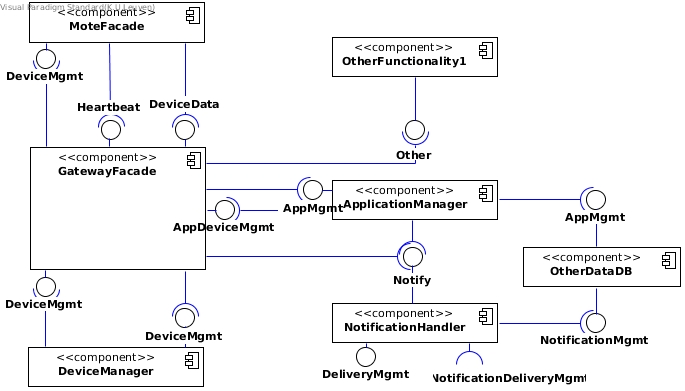
\includegraphics[width=1.00\textwidth]{component-diagram-1}
        	\caption{Component-and-connector diagram of this decomposition.}
            \label{fig:it1-cc_main}
        \end{figure}

        \noindent The responsibilities of the components are as follows:

    \subparagraph{ApplicationManager}
        Responsible for deactivating applications and after this action calls method of
        \texttt{the NotificationHandler} to send notification to a customer organisation.
        When \texttt{the ApplicationManager} detects that application uses failed pluggable devices,
        then the notification is sent to an application.

        set redundancy in the available pluggable devices??
        (Av3) ???? check mandatory user roles

    \subparagraph{Database}
        General database for other data. For instance the Database storages the data
        of notifications (Av3).

    \subparagraph{GatewayFacade}
        Receives heartbeats from pluggable devices and sends heartbeats/device lists.
        \texttt{The GatewayFacade} sends commands to \texttt{the ApplicationManager}
        to shutdown applications, if is it needed. \\

        send notification trigger ???(Av3)\\
        forward data to applications

    \subparagraph{MoteFacade}
        Sends heartbeats from pluggable devices to\texttt{the PluggableDeviceFacade}.

    \subparagraph{NotificationHandler}
        Responsible for send notifications to infrastructure owner, customer organisation
        and applications (Av3). \\
        stored by system \(->\) contact DB? \\
        lookup communication channel \\
        users choose delivery method?

    \subparagraph{PluggableDeviceFacade}
        Sends heartbeats to \texttt{the MoteFacade}.

    \subparagraph{PluggableDeviceManager}
        Checks list of devices and see if there are pluggable devices for applications.
        \texttt{the PluggableDeviceManager} contains application preferences (e.g. amount of sensors required) and
        can send command to deactivate application.
        Send information about new/needed hardware is detected to \texttt{the GatewayFacade}, that sends command to
        reactivate application.
        check redundancy in the available pluggable devices??? is not the same like first sentence???

    % \paragraph{Behaviour}
    % A SEQUENCE DIAGRAM WOULD BE USEFUL FOR
    % UC11: shows how the gateway checks if devices are initialised
    % UC14: shows how applications can get deactivated

    \paragraph{Deployment}
        Figure \ref{fig:it1-depl_main} shows the allocation of components
        to physical nodes.

        \begin{figure}[!htp]
        	\centering
        	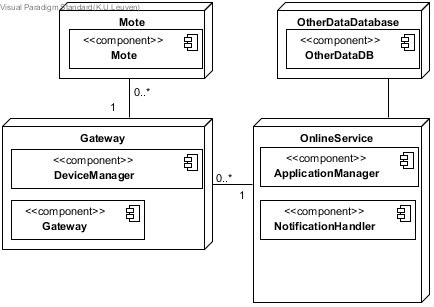
\includegraphics[width=1.00\textwidth]{deployment-diagram-1}
        	\caption{Deployment diagram of this decomposition.}\label{fig:it1-depl_main}
        \end{figure}


\subsection{Interfaces for child modules}\label{add1-interfaces}
    This section describes the interfaces assigned to the components defined
    in the section above. Per interface, we list its methods by means of its
    syntax. The data types used in these interfaces are defined in the following section. \\

    \noindent Each method shows which (part of a) quality attribute or use case caused
    a need for the method. However, this does not mean that a method is
    only to be used to satisfy that quality  attribute or use case, it could
    be used for other causes not yet mentioned here.

    \subsubsection{ApplicationManager}
        \begin{itemize}
            \item ForwardData
            \begin{itemize}
                \item \texttt{void sendData(PluggableDeviceData data)}
                \begin{itemize}
                    \item Effect: Send pluggable device data to an application that wants to use it
                    \item Created for:
                \end{itemize}
            \end{itemize}

            \item AppMgmt
            \begin{itemize}
                \item \texttt{void deactivateApplicationInstance(int applicationInstanceID)}
                \begin{itemize}
                    \item Effect: Deactivates a running instance of an application.
                    \item Created for:
                \end{itemize}
                \item \texttt{void activateApplicationInstance(int applicationInstanceID)}
                \begin{itemize}
                    \item Effect: Activates a new instance of an application.
                    \item Created for:
                \end{itemize}
            \end{itemize}
        \end{itemize}

    \subsubsection{Database}
        \begin{itemize}
            \item NotificationMgmt
            \begin{itemize}
                \item \texttt{int storeNotification(NotificationData data)}
                \begin{itemize}
                    \item Effect: Stores a new notification entry in the database. Returns the id of the new notification.
                    \item Created for:
                \end{itemize}
                \item \texttt{void updateNotification(NotificationData data)}
                \begin{itemize}
                    \item Effect: Updates an existing notification (e.g. change status to "sent").
                    \item Created for:
                \end{itemize}
                \item \texttt{int lookupNotificationChannelForUser(int userID)}
                \begin{itemize}
                    \item Effect: Returns the type of communication channel a user prefers.
                                  Different communication channels are mapped to integers.
                    \item Created for:
                \end{itemize}
            \end{itemize}

            \item AppDataMgmt
            \begin{itemize}
                \item \texttt{void updateApplication(ApplicationData data)}
                \begin{itemize}
                    \item Effect: Updates an application in the database (e.g. change state to 'inactive').
                    \item Created for:
                \end{itemize}
                \item \texttt{void updateSubscription(SubscriptionData data)}
                \begin{itemize}
                    \item Effect: Updates a subscription in the database (e.g. change state to 'disabled').
                    \item Created for:
                \end{itemize}
            \end{itemize}
        \end{itemize}

    \subsubsection{GatewayFacade}
        \begin{itemize}
            \item MoteDataMgmt
            \begin{itemize}
                \item \texttt{void sendHeartbeat(int moteID, List<PluggableDeviceInfo> devices)}
                \begin{itemize}
                    \item Effect: Sends a heartbeat to a certain gateway with information about operational devices.
                    \item Created for:
                \end{itemize}
            \end{itemize}

            \item DeviceMgmt
            \begin{itemize}
                \item \texttt{List<DeviceInfo> getConnectedDevices()}
                \begin{itemize}
                    \item Effect: Describe the effect of calling this operation.
                    \item Created for:
                \end{itemize}
                \item \texttt{void timerExpired(int deviceID)}
                \begin{itemize}
                    \item Effect: Lets the gateway know that a timer for pluggable device or mote has expired.
                                  This will generate a notification for an infrastructure owner.
                    \item Created for:
                \end{itemize}
                \item \texttt{void deactivateApplicationInstance(int applicationInstanceID)}
                \begin{itemize}
                    \item Effect: Deactivates a certain application. This could happen when
                                  mandatory pluggable devices for the application are missing.
                    \item Created for:
                \end{itemize}
                \item \texttt{void reactivateApplicationInstance(int applicationInstanceID)}
                \begin{itemize}
                    \item Effect: Reactivate an application instance. This could happen
                                  automatically after a broken sensor has been replaced.
                    \item Created for:
                \end{itemize}
            \end{itemize}

            \item AppDeviceMgmt
            \begin{itemize}
                \item \texttt{bool areEssentialDevicesOperational(int applicationID)}
                \begin{itemize}
                    \item Effect: Returns true if all essential devices for the application
                                  with id "applicationID" are operational.
                    \item Created for:
                \end{itemize}
            \end{itemize}
        \end{itemize}

    \subsubsection{MoteFacade}
        \begin{itemize}
            \item PluggableDeviceDataMgmt
            \begin{itemize}
                \item \texttt{List<DeviceInfo> getConnectedDevices()}
                \begin{itemize}
                    \item Effect: Returns a list of information about devices that are connected to the mote.
                    \item Created for:
                \end{itemize}
            \end{itemize}
        \end{itemize}

    \subsubsection{NotificationHandler}
        \begin{itemize}
            \item Notify
            \begin{itemize}
                \item \texttt{void notify(int userID, String message)}
                \begin{itemize}
                    \item Effect: Describe the effect of calling this operation.
                    \item Created for:
                \end{itemize}
            \end{itemize}

            \item DeliveryMgmt
            \begin{itemize}
                \item \texttt{void sendAcknowledgement(int notificationID)}
                \begin{itemize}
                    \item Effect: Sends an acknowledgement to the system for a certain notification.
                    \item Created for:
                \end{itemize}
            \end{itemize}
        \end{itemize}

    \subsubsection{External notification delivery serivce}
        \begin{itemize}
            \item NotificationDeliveryMgmt
            \begin{itemize}
                \item \texttt{void notify(JSONObject data)}
                \begin{itemize}
                    \item Effect: Deliver a notification to an end user using a specific delivery service.
                    \item Created for:
                \end{itemize}
            \end{itemize}
        \end{itemize}

    \subsubsection{PluggableDeviceManager}
        \begin{itemize}
        	\item DeviceListMgmt
        	\begin{itemize}
        		\item \texttt{void sendHeartbeat(int moteID, List<PluggableDeviceInfo> devices)}
        		\begin{itemize}
        			\item Effect: Send a heartbeat from a mote to check/update timers for operational devices.
        			\item Created for:
        		\end{itemize}
        		\item \texttt{bool areEssentialDevicesOperational(int applicationID)}
        		\begin{itemize}
        			\item Effect: Returns true if all essential devices for the application
                                  with id "applicationID" are operational.
        			\item Created for:
        		\end{itemize}
        	\end{itemize}
        \end{itemize}


\subsection{Data type definitions}
    This section defines the data types used in the interface descriptions above.

    \paragraph{PluggableDeviceData}
              contains data from a pluggable device at a certain point in time
              (value, type, date) (e.g. a sensor reading, an actuator status)
    \paragraph{PluggableDeviceSettings}
              contains settings for a pluggable device (power status,
              data update rate, ...)
    \paragraph{PluggableDeviceInfo}
              contains information about a pluggable device (device id,
              power status, data update rate, ...)
    \paragraph{NotificationData}
              contains data about a notification (message text, recipient,
              communication channel, date, status, source, ...).
    \paragraph{ApplicationData}
              contains data about an application instance (instance id, running status, ...)
    \paragraph{SubscriptionData}
              contains data about a subscription (subscription id, subscription status,
              subscription period, ...).


\subsection{Verify and refine}
    \noindent The selected architectural drivers have been handled completely
    in this decomposition.
    This section describes per component which (parts of) the remaining
    requirements it is responsible for. If requirements are split in
    multiple parts, this is indicated by the addition of a letter
    (or number, depending on the structure of the requirement) after their title.

    \paragraph{ApplicationManager}
        \begin{itemize}
            \item \emph{Av2}: Application failure \\
                   Prevention: a, b \\
                   Detection: a, b, c \\
                   Resolution: a, b, c
           \item \emph{P1}: Large number of users: c
           \item \emph{M1}: Integrate new sensor or actuator manufacturer: 1.c, 2.a
           \item \emph{M2}: Big data analytics on pluggable data and/or application usage data: d, e
           \item \emph{U1}: Application updates: a, b, c, d
           \item \emph{U2}: Easy Installation: e
           \item \emph{UC12}: Perform actuation command
           \item \emph{UC17}: Activate an application: 3, 4
        \end{itemize}

    \paragraph{Database}
        \begin{itemize}
          	\item None
        \end{itemize}

    \paragraph{GatewayFacade}
        \begin{itemize}
            \item \emph{Av1}: Communication between SIoTIP gateway and Online Service \\
                               Resolution: b, c, d
            \item \emph{M1}: Integrate new sensor or actuator manufacturer: 1.a, 2.b
            \item \emph{U2}: Easy Installation: a, c, d
            \item \emph{UC11}: Send pluggable device data: 1
        \end{itemize}

    \paragraph{MoteFacade}
        \begin{itemize}
            \item \emph{M1}: Integrate new sensor or actuator manufacturer: 1.a, 2.b
            \item \emph{U2}: Easy Installation: b, c, d
            \item \emph{UC04}: Install mote: 1, 2
            \item \emph{UC05}: Uninstall mote: 1
            \item \emph{UC06}: Insert a pluggable device into a mote: 2
            \item \emph{UC07}: Remove a pluggable device from its mote: 2
            \item \emph{UC11}: Send pluggable device data: 1
        \end{itemize}

    \paragraph{NotificationHandler}
        \begin{itemize}
            \item \emph{UC16}: Consult notification message: 5
            \item \emph{UC17}: Activate an application: 5, 6
        \end{itemize}

    \paragraph{OtherFunctionality1}
        \begin{itemize}
            \item \emph{Av1}: Communication between SIoTIP gateway and Online Service \\
                               Detection: a, b, c, d
                               Resolution: a
           	\item \emph{P1}: Large number of users: a
            \item \emph{P2}: Requests to the pluggable data database
            \item \emph{M1}: Integrate new sensor or actuator manufacturer: 1.d
            \item \emph{M2}: Big data analytics on pluggable data and/or application usage data: a
            \item \emph{U2}: Easy Installation: e
            \item \emph{UC01}: Register a customer organisation
            \item \emph{UC02}: Register an end-user
            \item \emph{UC03}: Unregister an end user
            \item \emph{UC04}: Install mote: 3
            \item \emph{UC05}: Uninstall mote: 2.b
            \item \emph{UC06}: Insert a pluggable device into a mote: 3: topology part; alternative 3a.1.b
            \item \emph{UC07}: Remove a pluggable device from its mote: 3.b
            \item \emph{UC08}: Initialise a pluggable device: 1, 2, 4
            \item \emph{UC09}: Configure pluggable device access rights
            \item \emph{UC10}: Consult and configure the topology
            \item \emph{UC11}: Send pluggable device data: 3
            \item \emph{UC13}: Configure pluggable device
            \item \emph{UC16}: Consult notification message: 1, 2, 3, 4
            \item \emph{UC17}: Activate an application: 1, 2
            \item \emph{UC19}: Subscribe to application
            \item \emph{UC20}: Unsubscribe from application
            \item \emph{UC21}: Send invoice
            \item \emph{UC22}: Upload an application
            \item \emph{UC23}: Consult application statistics
            \item \emph{UC24}: Consult historical data
            \item \emph{UC25}: Access topology and available devices
            \item \emph{UC26}: Send application command or message to external front-end
            \item \emph{UC27}: Receive application command or message to external front-end
            \item \emph{UC28}: Log in
            \item \emph{UC29}: Log out
        \end{itemize}

    \paragraph{PluggableDeviceFacade}
        \begin{itemize}
        	\item \emph{U2}: Easy Installation: d
        \end{itemize}

    \paragraph{PluggableDeviceManager}
        \begin{itemize}
            \item \emph{U2}: Easy Installation: c, d
            \item \emph{UC04}: Install mote: 4
            \item \emph{UC05}: Uninstall mote: 2
            \item \emph{UC06}: Insert a pluggable device into a mote: 3: uninitialised part; alternative 3a.1 3a.2 3a.4; 4
            \item \emph{UC07}: Remove a pluggable device from its mote: 3.a, 3.c
            \item \emph{UC08}: Initialise a pluggable device: 3
            \item \emph{UC11}: Send pluggable device data: 2, 3a
        \end{itemize}

    \newpage
    \section{Decomposition 2: OtherFunctionality1 (M1, P2, UC11)}

\subsection{Module to decompose}
    In this run we decompose OtherFunctionality1.


\subsection{Selected architectural drivers}
    The non-functional drivers for this decomposition are:
    \begin{itemize}
    	\item \emph{M1}: Integrate new sensor or actuator manufacturer
        \item \emph{P2}: Requests to the pluggable data database
    \end{itemize}

    \noindent The related functional drivers are:
    \begin{itemize}
        \item \emph{UC11}: Send pluggable device data (P2) \\
              This use case stores pluggable device data in the pluggable device data storage.
              This could be a sensor reading or an actuator status.
    \end{itemize}

    \paragraph{Rationale}
    We chose M1 as it was one of the remaining quality attributes with high priority.
    M1's focus on easily introducing new types of devices to the system is very important
    because of the fast growing market for IoT and development of applications for IoT.
    Thus, we want to handle this quality attribute before U2 (the other remaining
    attribute with high priority), as we presume that customer organisations
    are more interested in using new devices than the effort it takes for
    infrastructure owners to install the devices. \\
    We also chose P2 because it is strongly related to M1; the whole data flow from
    devices to storage/applications needs to exist before modifications can even be made.
    This combination of M1 and P2 would force us to handle processing and
    storage of data while making the involved components as simple as possible to modify.


\subsection{Architectural design}
    This section describes what needs to be done to satisfy the requirements for
    this decomposition and how involved problems/obstacles are solved.
    % Tactics:
    %     Limit event response? reply within response measure deadlines
    %     Prioritize events
    %     Introduce concurrency
    %     Schedule resources

    % Tactics M1:
    %     reduce size of modules: split module

    \paragraph{M1: Handling new types of pluggable devices}
        The new types of sensor or actuator data should be transmitted, processed and stored,
        and should be made available to applications. The infrastructure managers must be able to initialize the new type of pluggable device
        (UC8 : Initialise a pluggable device), configure access rights for these devices (UC9 : Con-
        figure pluggable device access rights), and view detailed information about the new type
        of pluggable device (UC10 : Consult and configure the topology).

        The developers have to make changes to: component1, component2, datatype X.
        The new type of sensor needs to be able to be initialised so that it can send data.
        Thus, the PluggableDeviceFacade code that initialises devices should be updated for
        each new type of sensor. The PluggableDeviceData datatype should be updated to
        represent the new type of data. In this case, the new type will have to be added
        to the database that contains all different types of sensor data.

    \paragraph{M1: Data conversions}
        The pluggable data processing subsystem should be extended with relevant data conver-
        sions, e.g. converting temperature in degrees Fahrenheit to degrees Celsius.
        \texttt{The PluggableDeviceDataConverter} is resposible for converting data
        in system, for instance converting temperature in degrees Fahrenheit
        to degrees Celsius. System has to work with relevant data,
        otherwise problem may arise.

    \paragraph{M1: Usage of new data by applications}
        The available applications can be updated to use any new pluggable devices.
        This is possible through the RequestData interface provided by PluggableDeviceDataScheduler.
        The application manager can get device data from the PluggableDeviceDB and return this
        data to applications in the PluggableDeviceData datatype. This datatype can easily be
        updated for new types of pluggable devices.

    \paragraph{M1: Configuration of new device by infrastructure owners}
        Initialisation: IO triggers the initialise() method which has been
        updated for the new pluggable device -> OK\\
        Configure access rights: has absolutely fucking nothing to do with the
        new sensor type -> OK \\
        Consult and configure topology: same as configure access rights

    \paragraph{P2: Scheduling}
        - In normal mode, the database processes incoming requests in a first-in-first-out order.
        - If the system fails to comply to the deadlines specified below, it goes in overload mode: requests
            are handled in the order that returns the system to normal mode the fastest, taking into
            account:
            ∗ the nature of the requests: storing new pluggable data (UC11 : Send pluggable device
            data) has priority over specific lookup queries (e.g. retrieving most recent measurement
            for a few sensors), which in turn have priority over broad queries (e.g. retrieving all sensor
            data for the last month).
            ∗ the priority of an application: requests from applications marked as critical by their sub-
            scribers are processed before non-critical applications.
        - Also a mechanism should be in place to avoid starvation of any type of request.

        dynamic priority scheduling \\
        tactics: schedule resource, prioritize events, also limit event response?\\
        starvation avoidance

    \paragraph{P2: Pluggable data separation}
        The processing of (large amounts of) requests concerning pluggable data has no impact on
        requests concerning other data, e.g. available applications.

        "pluggable data has no impact on other data"
        two databases

    \subsubsection{Alternatives considered}
        \paragraph{P2: Alternatives for Scheduling}
        In overload mode, a high priority process will run before a low priority process. 
        It can cuase that the low priority process will never be scheduled.
        Our scheduling algorithms will contain code to guarantee that all processes will 
        receive a minimum amount of each important resource (e.g. CPU time) in order to avoid starvation.


\subsection{Instantiation and allocation of functionality}
    This section describes the new components which instantiate our solutions described
    in the section above and how components are deployed on physical nodes. \\
    Unless stated otherwise the responsibilities assigned in the first decomposition are unchanged.

    \paragraph{Decomposition}
        Figure \ref{fig:it2-cc_main} shows the components resulting from the
        decomposition in this run.

        \begin{figure}[!h]
        	\centering
            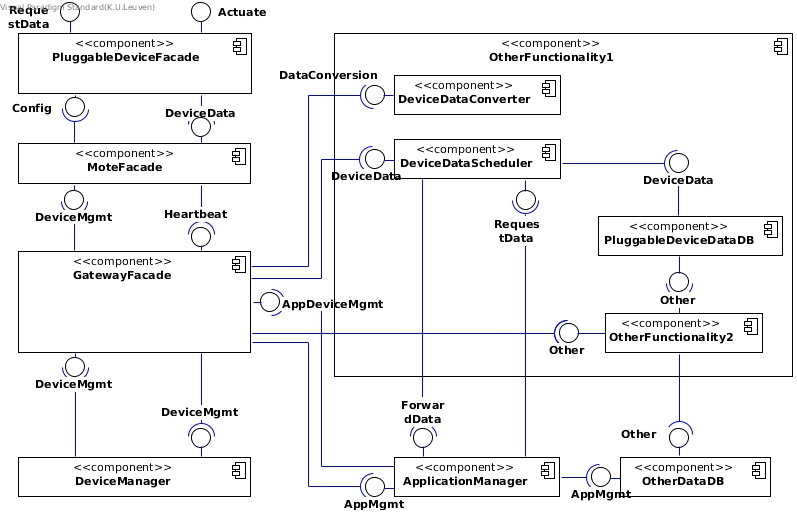
\includegraphics[width=1\textwidth]{component-diagram-2}
        	\caption{Component-and-connector diagram of this decomposition.}
            \label{fig:it2-cc_main}
        \end{figure}

        \noindent The responsibilities of the components are as follows:

    \subparagraph{PluggableDeviceDB}
        stores data related to pluggable devices. In \texttt{the PluggableDeviceDB}
        is stored basic information about devices.

    \subparagraph{PluggableDeviceDataScheduler}
        \texttt{the PluggableDeviceDB} receives a large amount of parallel request
        and it is neccesary to handle with that.
        \texttt{The PluggableDeviceDataScheduler} is resposnsible for scheduling jobs
        that interact with database. Jobs are processed in a first-in-first-out order normaly.
        In case te overload mode is detected, jobs are proccesed in  the  order
        that  returns  the  system. In case the data has to be saved,
        \texttt{The PluggableDeviceDataScheduler} call method for saving the data, that
         \texttt{the PluggableDeviceDB} provides.

    \subparagraph{PluggableDeviceDataConverter}
       is component for conversions of new type of data of new type of device (M1).
       For instance converting temperature is very useful in the system.

    % \paragraph{Behaviour}
        % A SEQUENCE DIAGRAM WOULD BE USEFUL FOR
        % UC11: shows how the gateway checks if devices are initialised
        % UC14: shows how applications can get deactivated

    \paragraph{Deployment}
        Figure \ref{fig:it2-depl_main} shows the allocation of components
        to physical nodes.

        \begin{figure}[!h]
        	\centering
        	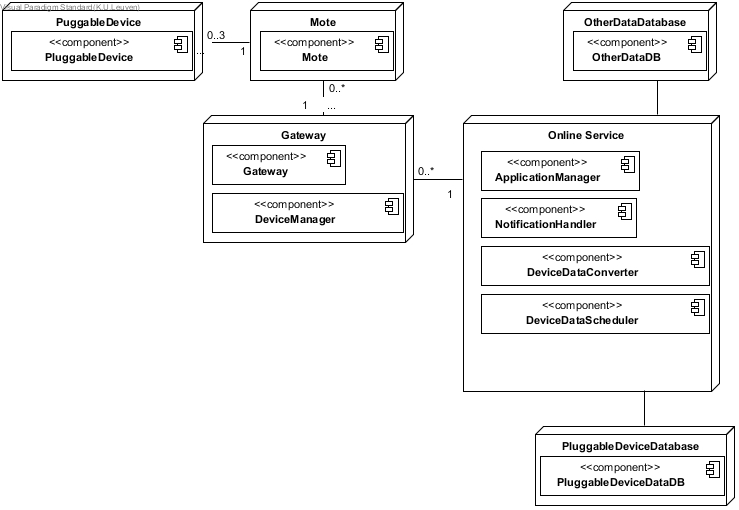
\includegraphics[width=1\textwidth]{deployment-diagram-2}
        	\caption{Deployment diagram of this decomposition.
        	}\label{fig:it2-depl_main}
        \end{figure}


\subsection{Interfaces for child modules}\label{add2-interfaces}
    This section describes the interfaces assigned to the components defined
    in the section above. Per interface, we list its methods by means of its
    syntax. The data types used in these interfaces are defined in the following section. \\

    \noindent Each method shows which (part of a) quality attribute or use case caused
    a need for the method. However, this does not mean that a method is
    only to be used to satisfy that quality  attribute or use case, it could
    be used for other causes not yet mentioned here.

    \noindent The interfaces and methods defined here are to be seen as an
    extension of the interfaces defined in previous sections, unless
    explicitly stated otherwise.

    \subsubsection{GatewayFacade}
        \begin{itemize}
            \item MoteDataMgmt, last defined in section \ref{add1-interfaces}
            \begin{itemize}
                \item \texttt{void sendData(PluggableDeviceData data)}
                \begin{itemize}
                    \item Effect: Sends pluggable device data to the connected mote.
                    \item Created for:
                \end{itemize}
            \end{itemize}

            \item DeviceMgmt, last defined in section \ref{add1-interfaces}
            \begin{itemize}
                \item \texttt{void initialiseDevice(int deviceID, PluggableDeviceSettings settings)}
                \begin{itemize}
                    \item Effect: Initialises a pluggable device for use with the system.
                    \item Created for:
                \end{itemize}
            \end{itemize}

            \item AppDeviceMgmt, last defined in section \ref{add1-interfaces}
            \begin{itemize}
                \item \texttt{void configurePluggableDevice(int deviceID, PluggableDeviceSettings settings)}
                \begin{itemize}
                    \item For: Use case 11 step 3.b
                    \item Effect: Causes certain settings to be set on a pluggable
                          device that the gateway is connected to.
                    \item Created for:
                \end{itemize}
            \end{itemize}
        \end{itemize}

    \subsubsection{MoteFacade}
        \begin{itemize}
            \item PluggableDeviceDataMgmt, last defined in section \ref{add1-interfaces}
            \begin{itemize}
                \item \texttt{void sendData(PluggableDeviceData data)}
                \begin{itemize}
                    \item Effect: Sends pluggable device data to the connected mote.
                    \item Created for:
                \end{itemize}
            \end{itemize}

            \item PluggableDeviceMgmt
            \begin{itemize}
                \item \texttt{void initialise(int deviceID, PluggableDeviceSettings settings)}
                \begin{itemize}
                    \item Effect: Initialises a connected pluggable device according to some settings
                    \item Created for:
                \end{itemize}
            \end{itemize}
        \end{itemize}

    \subsubsection{PluggableDeviceFacade}
        \begin{itemize}
        	\item PluggableDeviceMgmt
        	\begin{itemize}
                \item \texttt{void initialise(PluggableDeviceSettings settings)}
                \begin{itemize}
                    \item Effect: Initialises the pluggable device according to some settings
                    \item Created for:
                \end{itemize}
        	\end{itemize}
        \end{itemize}

    \subsubsection{PluggableDeviceManager}
        \begin{itemize}
        	\item DeviceListMgmt, last defined in section \ref{add1-interfaces}
        	\begin{itemize}
        		\item \texttt{bool isDeviceInitialised(int deviceID)}
        		\begin{itemize}
        			\item Effect: Returns true if the device with id "deviceID" has been initialized.
        			\item Created for:
        		\end{itemize}
        	\end{itemize}
        \end{itemize}

    \subsubsection{PluggableDeviceDataScheduler}
        \begin{itemize}
            \item RequestData
            \begin{itemize}
                \item \texttt{List<PluggableDeviceData> requestData(int applicationID, int deviceID, DateTime from, DateTime to)}
                \begin{itemize}
                    \item Effect: Request data from a specific device in a certain time period
                    \item Created for:
                \end{itemize}
            \end{itemize}

            \item PluggableDeviceDataMgmt
            \begin{itemize}
                \item \texttt{void sendData(PluggableDeviceData data)}
                \begin{itemize}
                    \item Effect: Sends pluggable device data to the scheduler to be processed.
                    \item Created for:
                \end{itemize}
            \end{itemize}
        \end{itemize}

    \subsubsection{PluggableDeviceDB}
        \begin{itemize}
            \item PluggableDeviceDataMgmt
            \begin{itemize}
                \item \texttt{void sendData(PluggableDeviceData data)}
                \begin{itemize}
                    \item Effect: Sends pluggable device data to the DB to be stored.
                    \item Created for:
                \end{itemize}
                \item \texttt{List<PluggableDeviceData> getData(int deviceID, DateTime from, DateTime to)}
                \begin{itemize}
                    \item Effect: Returns data from a specific device in a certain time period.
                    \item Created for:
                \end{itemize}
                \item \texttt{List<int> getApplicationsForDevice(int deviceID)}
                \begin{itemize}
                    \item Effect: Returns a list of applications that can use the device with id "deviceID."
                    \item Created for:
                \end{itemize}
            \end{itemize}
        \end{itemize}


\subsection{Data type definitions}
    This section defines new data types that are used in the interface descriptions above.

    \paragraph{DateTime} Represents an instant in time, typically expressed as a date and time of day.


\subsection{Verify and refine}
    \noindent The selected architectural drivers have been handled completely
    in this decomposition.
    This section describes per component which (parts of) the remaining
    requirements it is responsible for. If requirements are split in
    multiple parts, this is indicated by the addition of a letter
    (or number, depending on the structure of the requirement) after their title.

    \paragraph{ApplicationManager}
        \begin{itemize}
            \item \emph{Av2}: Application failure \\
                   Prevention: a, b \\
                   Detection: a, b, c \\
                   Resolution: a, b, c
           \item \emph{P1}: Large number of users: c
           \item \emph{M2}: Big data analytics on pluggable data and/or application usage data: d, e
           \item \emph{U1}: Application updates: a, b, c, d
           \item \emph{U2}: Easy Installation: e
           \item \emph{UC12}: Perform actuation command
           \item \emph{UC17}: Activate an application: 3, 4
        \end{itemize}

    \paragraph{Database}
        \begin{itemize}
          	\item None
        \end{itemize}

    \paragraph{GatewayFacade}
        \begin{itemize}
            \item \emph{Av1}: Communication between SIoTIP gateway and Online Service \\
                               Resolution: b, c, d
            \item \emph{U2}: Easy Installation: a, c, d
        \end{itemize}

    \paragraph{MoteFacade}
        \begin{itemize}
            \item \emph{U2}: Easy Installation: b, c, d
            \item \emph{UC04}: Install mote: 1, 2
            \item \emph{UC05}: Uninstall mote: 1
            \item \emph{UC06}: Insert a pluggable device into a mote: 2
            \item \emph{UC07}: Remove a pluggable device from its mote: 2
        \end{itemize}

    \paragraph{NotificationHandler}
        \begin{itemize}
            \item \emph{UC16}: Consult notification message: 5
            \item \emph{UC17}: Activate an application: 5, 6
        \end{itemize}

    \paragraph{OtherFunctionality2}
        \begin{itemize}
            \item \emph{Av1}: Communication between SIoTIP gateway and Online Service \\
                               Detection: a, b, c, d
                               Resolution: a
           	\item \emph{P1}: Large number of users: a
            \item \emph{M2}: Big data analytics on pluggable data and/or application usage data: a
            \item \emph{U2}: Easy Installation: e
            \item \emph{UC01}: Register a customer organisation
            \item \emph{UC02}: Register an end-user
            \item \emph{UC03}: Unregister an end user
            \item \emph{UC04}: Install mote: 3
            \item \emph{UC05}: Uninstall mote: 2.b
            \item \emph{UC06}: Insert a pluggable device into a mote: 3: topology part; alternative 3a.1.b
            \item \emph{UC07}: Remove a pluggable device from its mote: 3.b
            \item \emph{UC08}: Initialise a pluggable device: 1, 2, 4
            \item \emph{UC09}: Configure pluggable device access rights
            \item \emph{UC10}: Consult and configure the topology
            \item \emph{UC13}: Configure pluggable device
            \item \emph{UC16}: Consult notification message: 1, 2, 3, 4
            \item \emph{UC17}: Activate an application: 1, 2
            \item \emph{UC19}: Subscribe to application
            \item \emph{UC20}: Unsubscribe from application
            \item \emph{UC21}: Send invoice
            \item \emph{UC22}: Upload an application
            \item \emph{UC23}: Consult application statistics
            \item \emph{UC24}: Consult historical data
            \item \emph{UC25}: Access topology and available devices
            \item \emph{UC26}: Send application command or message to external front-end
            \item \emph{UC27}: Receive application command or message to external front-end
            \item \emph{UC28}: Log in
            \item \emph{UC29}: Log out
        \end{itemize}

    \paragraph{PluggableDeviceDB}
        \begin{itemize}
            \item \emph{M2}: Big data analytics on pluggable data and/or application usage data: b
        \end{itemize}

    \paragraph{PluggableDeviceFacade}
        \begin{itemize}
        	\item \emph{U2}: Easy Installation: d
        \end{itemize}

    \paragraph{PluggableDeviceManager}
        \begin{itemize}
            \item \emph{U2}: Easy Installation: c, d
            \item \emph{UC04}: Install mote: 4
            \item \emph{UC05}: Uninstall mote: 2
            \item \emph{UC06}: Insert a pluggable device into a mote: 3: uninitialised part; alternative 3a.1 3a.2 3a.4; 4
            \item \emph{UC07}: Remove a pluggable device from its mote: 3.a, 3.c
            \item \emph{UC08}: Initialise a pluggable device: 3,
        \end{itemize}

    \paragraph{PluggableDeviceDataScheduler}
        \begin{itemize}
            \item \emph{P1}: Large number of users: b
            \item \emph{M2}: Big data analytics on pluggable data and/or application usage data: b, c
        \end{itemize}

    \newpage
    % \section{Decomposition 3: U2, UC4, UC6, UC9, UC10, UC17, UC19.7-11}

\subsection{Elements/Subsystem to decompose/expand}
    In this run we decompose/expand ...


\subsection{Selected architectural drivers}
    The non-functional drivers for this decomposition are:
    \begin{itemize}
    	\item \emph{U2}: Easy installation
    \end{itemize}

    The related functional drivers are:
    \begin{itemize}
        \item \emph{UC4}: Install mote \\
              Short description
        \item \emph{UC6}: Insert a pluggable device into a mote \\
              Short description
        \item \emph{UC9}: Configure pluggable device access rights \\
              Short description
        \item \emph{UC10}: Consult and configure topology \\
              Short description
        \item \emph{UC17}: Activate an application \\
              Short description
        \item \emph{UC19}: Subscribe to application \\
              Short description
    \end{itemize}


\subsection{Architectural design}
    This section describes what needs to be done to satisfy the requirements for
    this decomposition and how involved problems/obstacles are solved.

    topology
        gateways(id, floor, room_number, wall, status)
        motes(id, gateway_id, floor, room_number, status)
        pluggable_devices(id, mote_id, gateway_id, status, physical location)
        pluggable_devices_redundancies(deviceID1, deviceID2)

    access rights
        rights(id, origranisation_id, device_id, can_read, can_configure, can_send_actuation_command)

    \paragraph{U2: Gateway installation}
        The gateway should not require any configuration, other than being connected
        to the local wired or WiFi network, after it is plugged into an electrical
        socket. An infrastructure owner should be able get the SIoTIP gateway
        up-and-running (connected) within 10 minutes given that the information
        (e.g. WiFi SSID and passphrase) is available to the person responsible for
        the installation. \\
        TODO: ask \\
        We need something that registers the gateway automatically with the
        online service after bootup. A connection to the internet is a constraint
        of the GatewayFacade.

    \paragraph{U2: Mote installation}
        Installing a new mote should not require more configuration than adding it
        to the topology. Adding new motes, sensors or actuators should not involve
        more than just starting motes, and plugging devices into motes – plug-and-play! TODO: ask \\
        Reintroducing a previously known mote, with the same pluggable devices attached to it,
        should not require any configuration. It is automatically re-added on
        its last known location on the topology. The attached pluggable devices
        are automatically initialised and configured with their last known
        configuration and access rights. \\
        Thing that need to happen automatically:
        *) mote should find the gateway (mote sends a broadcast message->ReceiveBroadcast)
        *) gateway should register the mote (DeviceManager update, store entry in DB)
        *) on reintroduction of motes: DeviceManager notices this, makes the gateway send a message to online service to reuse some old topology

        UC4:
            Remark : The mote is pre-congured to connect to a specic gateway by
             the hardware manufacturer. This linking process is out of scope for
             this assignment. Likewise, the automatic assignment of an IPv6 address
             to the mote is out of scope.

            if new mote:
                % 2. MoteFacade -> GatewayFacade: registerMote(moteID, IPAddress moteIPAddress)
                % 3. GatewayFacade -> DeviceManager: registerMote(moteID, IPAddress moteIPAddress)
                % 3. DeviceManager -> GatewayFacade -> PluggableDeviceDataScheduler: addMote(moteID, gatewayID, IPAddress moteIPAddress)
                                                    %  PluggableDeviceDataScheduler -> PluggableDeviceDB: addMote(moteID, gatewayID, IPAddress moteIPAddress)
                                                %   -> TopologyManager: addMote(infrastructureOwnerID, gatewayID, moteID) // status = unplaced
                                                    %  TopologyManager -> PluggableDeviceDataScheduler -> PluggableDeviceDB: addMoteInTopology(infrastructureOwnerID, gatewayID, moteID)
                % 4. DeviceManager -> GatewayFacade -> NotificationHandler: notify(infrastructureOwnerID, message)

        if reintroduced mote:
            It is automatically re-added on its last known location on the topology.
                % 3. DeviceManager -> GatewayFacade -> PluggableDeviceDataScheduler: reactivateMote(moteID)
                % 3. DeviceManager -> GatewayFacade -> TopologyManager: reactivateMote(moteID) // status = placed? (TODO ASK?), location is still there from the past, it was not removed

            The attached pluggable devices are automatically initialised and configured with their last known configuration.
            The attached pluggable devices are automatically initialised and configured with their last known access rights.
                Already done by DeviceManager, it detects the devices, updates DB, and configures the devices
                % 3. DeviceManager -> GatewayFacade -> PluggableDeviceDataScheduler: reactivateDevice(deviceID)


    \paragraph{U2: Pluggable device installation}
        Adding new sensors or actuators should require no further customer
        actions besides plugging it into the mote. Configurable sensors and
        actuators should have a working default configuration.
        Pluggable devices added to an already known mote are automatically
        added in the right location on the topology.
        Making (initialised) sensors and actuators available to customer
        organisations and applications should not require more effort than
        configuring access rights (cf. UC9). \\
        *) After devices are plugged in: connect to mote, set up default configurations
        *) if the mote is already known, the device is added to the right location on the topology
        *) need something for configuration of access rights, can only happen for initialised devices

        *) for reactivating last configurations: just set status to active and don't change configuration field, it will still be the same as in the past
            alternative: current_configuration and last_configuration in DB
            alternative: store all configurations on Gateway -> but it has bad resources
            alternative: store all versions on PluggableDeviceDB -> but lots of useless data then = extra work for db

        *) Pluggable devices added to an already known mote are automatically added in "the right location" on the topology.
            what exactly is a location?
            => when a pluggable device is connected to a new mote, the pluggable device gets the location of the mote by default

        UC6: insert a pluggable device into a mote
            mote is already installed

            when device is plugged into a mote:
                mote -> DeviceManager: registerDevice(id, type) (registers device as uninitialised)
                DeviceManager -> PluggableDeviceDatabase: addDevice(id, type, status) (status = uninitialised)
                DeviceManager -> TopologyManager: addDeviceToMote(deviceID, moteID, status) (status = unplaced) (sets the location to the same of the mote)
                DeviceManager -> NotificationHandler: newPluggableDevice

                In these methods, if the device already exists and is plugged in in another mote, clear the data

            if the device is a known previously active device (ON THE SAME MOTE):
                mote -> DeviceManager: registerDevice(id, type)

                ∗ marks the pluggable device as ‘active’: DB pluggable_devices
                    DeviceManager -> PluggableDeviceDataScheduler: reactivateDevice(deviceID)

                ∗ updates the topology: DB topology_pluggable_devices
                    DeviceManager -> TopologyManager: reactivateDevice(deviceID)

                ∗ configures the pluggable device with the last known access rights: DB permissions_pluggable_devices
                    % DeviceManager -> DeviceAccessRightsManager: reactivate(deviceID)
                    nothing needs to happen here, permission information will just not be used if the device is inactive
                                                  if the device is reactivated, the permissions are already there

                * configures the pluggable device with the last known configuration: DB pluggable_devices
                    DeviceManager -> PluggableDevice: setConfiguration(Map<String, String> lastKnownConfiguratoin) (lastKnown.. taken from DB)

                ∗ checks and activates applications which can now execute again:
                    DeviceManager -> ApplicationManager: checkPluggableDevices() something like this

                * send notification
                    DeviceManager -> NotificationHandler: reactivatedPluggableDevice

        UC9: configure pluggable device access rights
            1. InfrastructureOwnerClient -> InfrastructureOwnerFacade: getAccessRights()
                2. InfrastructureOwnerFacade -> DeviceManager: getPluggableDevices(infrastructureOwnerID)
                3. InfrastructureOwnerFacade -> AccessRightsManager: getAccessRights(pluggableDeviceID)
                4. InfrastructureOwnerFacade -> OtherFunctionality: getCustomerOrganisations(infrastructureOwnerID)
            6. InfrastructureOwnerClient -> InfrastructureOwnerFacade: setAccessRights/updateAccessRights(pluggableDeviceID, List<int> customerOrganisations)
                6. InfrastructureOwnerFacade -> DeviceManager: configureAccessRights(pluggableDeviceID, List<int> customerOrganisations)
                7.a. AccessRightsManager -> PluggableDeviceDatabase: updateDeviceAccessRights(deviceID, custOrg) / deleteAccessRights()
                7.b. AccessRightsManager -> ApplicationManager: checkAccessRights(custOrg)
                7.c. AccessRightsManager -> ApplicationManager: checkPluggableDevices(custOrg)


    \paragraph{U2: Easy applications}
        Applications should work out of the box if the required sensors and
        actuators are available. Only when mandatory end-user roles must be
        assigned, additional explicit configuration actions are required
        from a customer organisation (cf. UC17, UC19). \\
        *) if there is a subsription and new hardware is plugged in: need something to check
           if some application can be activated now
        *) need something to assign user roles to users during UC19

        UC17:
            application needs to be activated because new subscription, changed topology, new version of application

            ApplicationManager is triggered by something else do to the following: method activateApplication(applicationInstanceID)
            1. ApplicationManager -> UserRolesManager: checkMandatoryUserRoles(applicationInstanceID)
            2. ApplicationManager -> DeviceManager: checkPluggableDevices(applicationInstanceID)
            3. ApplicationManager -> GatewayFacade: activateApplication(applicationInstanceID) -> ApplicationSandbox component on gateway
            4. application.start();
            4. ApplicationManager -> InvoiceManager: activatedApplication(applicationInstanceID, custOrgID, date)
            5. ApplicationManager -> NotificationManager: activatedApplication(custOrgID)
            6. ApplicationManager -> UserRolesManager: List<User> getUsersWithRoles(custOrgID)
            6. ApplicationManager -> getInstallationInstructions(applicationID)
            6. ApplicationManager -> NotificationManager: notify(userID, message)

            TODO notifications for alternative scenario's

        UC19:
            2. CustomerOrganisationClient -> CustomerOrganisationFacade: List<Application> getApplicationsToSubscribe(custOrgID)
                   CustomerOrganisationFacade -> ApplicationManager: List<Application> getApplicationsToSubscribe(custOrgID)
            4. CustomerOrganisationClient -> CustomerOrganisationFacade: subscribeToApplication(custOrgID, applicationID)
            5. CustomerOrganisationFacade -> ApplicationManager: getMandatoryDevicesAndTopologyConfigurations(applicationID)
            6. TODO: The primary actor carries out the topology configuration ??????????????????????????????????????????????????????????????????????????????????
            7. CustomerOrganisationFacade -> ApplicationManager: getAllUserRoles(applicationID)
            8. CustomerOrganisationFacade -> UserRolesManager: getAllUsers(custOrgID)
            9. CustomerOrganisationClient -> CustomerOrganisationFacade: setUserRoles(custOrgID, map<String, String> userRoles)
                   CustomerOrganisationFacade -> UserRolesManager: setUserRoles(custOrgID, map<String, String> userRoles)
                   10. <- return value is next page for selection of criticality
            11. CustomerOrganisationClient -> CustomerOrganisationFacade: setCriticality(applicationID, bool isCritical)
                    12. CustomerOrganisationFacade -> ApplicationManager: setCriticality(applicationID, bool isCritical)
            13. CustomerOrganisationFacade -> SubscriptionManager: subscribe(customerOrganisationID, applicationID) // returns applicationInstanceID of new application instance, if the org is subscribed to a older version, automatically unsubscribe
            14. CustomerOrganisationFacade -> ApplicationManager: activateApplication(applicationInstanceID)


\subsection{Instantiation and allocation of functionality}
    This section describes the new components which instantiate our solutions described
    in the section above and how components are deployed on physical nodes. \\
    Unless stated otherwise the responsibilities assigned in the first decomposition are unchanged.

    \paragraph{Decomposition}
        Figure \ref{fig:FIGURELABEL} shows the components resulting from the
        decomposition in this run.

        \begin{figure}[!h]
        	\centering
            %\includegraphics[width=1\textwidth]{IMAGE FILE NAME}
        	\missingfigure[figwidth=0.8\textwidth]{Component-and-connector diagram of this decomposition}
        	\caption{Component-and-connector diagram of this decomposition.}
            \label{fig:FIGURELABEL}
        \end{figure}

        The responsibilities of the components are as follows:

    \subparagraph{Component}
        Short description of its responsibilities. (Relevant QA or UC)


    % \paragraph{Behaviour}
        % USEFUL SEQUENCE DIAGRAMS FOR CHOSEN USE CASES


    \paragraph{Deployment}
        Figure \ref{fig:FIGURELABEL} shows the allocation of components
        to physical nodes.

        \begin{figure}[!h]
        	\centering
        	%\includegraphics[width=0.8\textwidth]{IMAGE FILE NAME}
        	\missingfigure[figwidth=0.8\textwidth]{Deployment diagram}
        	\caption{Deployment diagram of this decomposition.}
            \label{fig:FIGURELABEL}
        \end{figure}


\subsection{Interfaces for child modules}\label{add2-interfaces}
    This section describes the interfaces assigned to the components defined
    in the section above. Per interface, we list its methods by means of its
    syntax. The data types used in these interfaces are defined in the following section. \\

    Each method shows which (part of a) quality attribute or use case caused
    a need for the method. However, this does not mean that a method is
    only to be used to satisfy that quality  attribute or use case, it could
    be used for other causes not yet mentioned here.

    The interfaces and methods defined here are to be seen as an
    extension of the interfaces defined in previous sections, unless
    explicitly stated otherwise.

    \subsubsection{DeviceDataScheduler}
        \begin{itemize}
            \item Devices, renamed DeviceData of decomposition-2
            \begin{itemize}
                \item \texttt{void addMote(int moteID, int gatewayID, IPAddress moteIPAddress)}
                    \begin{itemize}
                        \item Effect:
                        \item Created for: UC4.3
                    \end{itemize}
                \item \texttt{void reactivateMote(int moteID)}
                    \begin{itemize}
                        \item Effect:
                        \item Created for: UC4.3
                    \end{itemize}
            \end{itemize}

        	\item TopologyMgmt
        	\begin{itemize}
        		\item \texttt{void addMoteInTopology(int infrastructureOwnerID, int gatewayID, int moteID)}
        		\begin{itemize}
        			\item Effect:
        			\item Created for: UC4.3
        		\end{itemize}

                \item \texttt{void reactivateMoteInTopology(int moteID)}
                    \begin{itemize}
                        \item Effect: Sets status to placed.
                        \item Created for: UC4.3
                    \end{itemize}
        	\end{itemize}
        \end{itemize}

    \subsubsection{GatewayFacade}
        \begin{itemize}
            \item RegisterMote
            \begin{itemize}
                \item \texttt{void registerMote(int moteID, IPAddress moteIPAddress)}
                    \begin{itemize}
                        \item Effect: Uses the DeviceDataScheduler to add the new mote in the PluggableDeviceDatabase.
                              Uses the TopologyManager to add the mote in the topology of the infrastructure owner.
                              Uses the NotificationHandler to send a notification of this event to the infrastructure owner.
                        \item Created for: UC4.2
                    \end{itemize}
            \end{itemize}

            \item DeviceMgmt, last defined in section \ref{add1-interfaces}
            \begin{itemize}
                \item \texttt{void addMote(moteID, int gatewayID, IPAddress moteIPAddress)}
                \begin{itemize}
                    \item Effect:
                    \item Created for: UC11: UC4.3
                \end{itemize}
                \item \texttt{void reactivateMote(int moteID)}
                \begin{itemize}
                    \item Effect: Uses the DeviceDataScheduler to change the status of the mote to active.
                          Uses the TopologyManager to change the status of the mote to placed again.
                          Uses the NotificationHandler to send a notification of this event to the infrastructure owner.
                    \item Created for: UC4.3 - reintroduced mote
                \end{itemize}
            \end{itemize}
        \end{itemize}

    \subsubsection{PluggableDeviceDB}
        \begin{itemize}
        	\item DeviceMgmt
        	\begin{itemize}
        		\item \texttt{void addMote(int moteID, int gatewayID, IPAddress moteIPAddress)}
        		\begin{itemize}
        			\item Effect:
        			\item Created for: UC4.3
        		\end{itemize}
                \item \texttt{void reactivateMote(int moteID)}
                    \begin{itemize}
                        \item Effect:
                        \item Created for: UC4.3
                    \end{itemize}
        	\end{itemize}

        	\item TopologyMgmt
        	\begin{itemize}
        		\item \texttt{void addMoteInTopology(int infrastructureOwnerID, int gatewayID, int moteID)}
        		\begin{itemize}
        			\item Effect:
        			\item Created for: UC4.3
        		\end{itemize}
                \item \texttt{void reactivateMoteInTopology(int moteID)}
                    \begin{itemize}
                        \item Effect: Sets status to placed.
                        \item Created for: UC4.3
                    \end{itemize}
        	\end{itemize}

        \end{itemize}

    \subsubsection{DeviceManager}
        \begin{itemize}
        	\item DeviceMgmt
        	\begin{itemize}
        		\item \texttt{void registerMote(moteID, IPAddress moteIPAddress)}
        		\begin{itemize}
        			\item Effect: Sends a heartbeat from a mote to check/update timers for operational devices.
        			\item Created for: UC4.3
        		\end{itemize}
        	\end{itemize}
        \end{itemize}

    \subsubsection{TopologyManager}
        \begin{itemize}
        	\item TopologyMgmt
        	\begin{itemize}
        		\item \texttt{void addMote(infrastructureOwnerID, int gatewayID, int moteID)}
        		\begin{itemize}
        			\item Effect: // status = unplaced
        			\item Created for: UC4.3
        		\end{itemize}
                \item \texttt{void reactivateMote(int moteID)}
                    \begin{itemize}
                        \item Effect:
                        \item Created for: UC4.3
                    \end{itemize}
        	\end{itemize}
        \end{itemize}

\subsection{Data type definitions}
    This section defines new data types that are used in the interface descriptions above.

    \paragraph{DataType}
        Description of data type

    \newpage
    \section{Decomposition 4: Av2, UC12, UC25, UC26, UC27 (application execution subsystem)}


\subsection{Selected architectural drivers}
    The non-functional drivers for this decomposition are:
    \begin{itemize}
    	\item \emph{Av2}: Application failure
    \end{itemize}

    The related functional drivers are:
    \begin{itemize}
        \item \emph{UC12}: Perform actuation command \\
              Short description of the UC.
        \item \emph{UC13}: Configure pluggable device \\
              Short description of the UC.
        \item \emph{UC25}: Access topology and available devices \\
              Short description of the UC.
        \item \emph{UC24}: Consult historical data \\
              Short description of the UC.
        \item \emph{UC26}: Send application command or message to external front-end \\
              Short description of the UC.
        \item \emph{UC27}: Receive application command or message from external front-end \\
              Short description of the UC.
    \end{itemize}

    \paragraph{Rationale}
        At this point the remaining drivers were Av1, Av2, and P1,
        which all had medium priority. We chose decompositions 4, 5,
        and 6 based on the priorities of the use cases that are related to the quality attributes. \\
        The related use cases from now on are the ones that would use components
        that are going to be changed in the decomposition.


\subsection{Architectural design}
    This section describes what needs to be done to satisfy the requirements for
    this decomposition and how involved problems/obstacles are solved.

    % Pattern: Container
    %     Define a container to provide the execution environment for a
    %     component that supports the necessary technical infrastructure
    %     to integrate components into application-specific usage scenarios,
    %     and on specific system platforms, without tightly coupling
    %     the components with the applications or platforms.
    %
    %     Use the container to initialize and provide the runtime context for the
    %     components it manages. Define operations that enable component
    %     objects to access their connections to ports of other components,
    %     as well as to access common middleware services such as persistence,
    %     event notification, transactions, replication, load balancing,
    %     and security.

    \paragraph{Av2: Detection of failures}
        The system is able to autonomously detect failures of its individual
        application execution components, failing applications, and failing application containers. \\
        Upon detection, a SIoTIP system administrator is notified. \\
        The failure of an internal application execution component is detected within 30 seconds.
        Detection of failed hardware or crashed software happens within 5 seconds.
        SIoTIP system administrators are notified within 1 minute.\\

        To detect failures, we made use of the \texttt{Container} pattern.
        The application execution subsystem is composed of:
        \begin{itemize}
            \item \texttt{ApplicationContainer}
            \item \texttt{ApplicationContainerMonitor}
            \item \texttt{ApplicationContainerManager}
            \item \texttt{ApplicationExecutionSubsystemMonitor}
        \end{itemize}

        The \texttt{ApplicationContainer}s are deployed in groups on different nodes.

        \texttt{ApplicationContainer}: is a container/sandbox that has 1 running application instance
        \texttt{ApplicationContainerMonitor}: monitors the \texttt{ApplicationContainer} instances

        To detect failing applications, \texttt{ApplicationContainer} and \texttt{ApplicationContainerMonitor}
            ApplicationContainer -> ApplicationContainerMonitor: void applicationCrashed(id applicationInstanceID)

        To detect failling application containers, \texttt{ApplicationContainerMonitor}
            ApplicationContainerMonitor -> ApplicationContainer: Echo ping()
            -> we say container has crashed/failed when the following has no response:

        To detect failures of individual application execution components,
        This means that one of \texttt{ApplicationContainer}, \texttt{ApplicationContainerMonitor}, \texttt{ApplicationContainerManager} crashed.
        If the \texttt{ApplicationContainer} failed, then the \texttt{ApplicationContainerMonitor} would detect this.
        If one of the other two components failed, the \texttt{ApplicationExecutionSubsystemMonitor} is put in place to detect this.

        These components will be deployed on the Online Service and on gateways.
        Since gateways are weaker machines than the ones on the Online Service,
        the ApplicationContainer can be confgured differently for gateways.
        The ApplicationContainers will then have stricter limits on
        resources used of the node they are working on.

        % TODO: see after the decomposition if this is useful to us
        % (usage of memory, number of served requestst and so ) and some monitoring
        % system (component), that monitors container sends regularly request to this endpoint
        % and  collect this information about aplications

        % Application executing on Online Service failed & Application executing on Gateway failed
        %     -> ApplicationInstance has failed AND ApplicationContainer is still ok
        %        so ApplicationContainer sends message "application instance X has crashed"
        %
        %
        % Container of application instance crashed
        %     -> ApplicationContainer has failed
        %     -> ApplicationContainerMonitor notices this (no reply to pings maybe)
        %     -> ApplicationContainerMonitor sends a command to the ApplicationContainerManager to restart or ...
        %
        % One of the internal application execution components crashed
        %     Application execution subsystem = ApplicationContainer + ApplicationContainerMonitor + ApplicationContainerManager

    \paragraph{Av2: Resolution of application failures and application execution component failures}
        In case of application crash, the system autonomously restarts failed applications.
        If part of an application fails, the remaining parts remain operational,
        possibly in a degraded mode (graceful degradation). \\
        After 3 failed restarts the application is suspended, and the
        application developer and customer organisation are notified within 5 minutes.\\

        In case of failure of application execution components or an application
        container, a system administrator is notified. \\
        SIoTIP system administrators are notified within 1 minute.\\

        When an application instance fails, the ApplicationContainerMonitor detects this and
        sends a command to the ApplicationContainerManager to restart the application instance.
        The ApplicationContainerMonitor keeps track of how many times the
        application instance has been restarted after a failure. After 3 failed restarts, the monitor
        send a command to the ApplicationContainerManager to suspend the application instance and send
        a notification to the application developers of the application and to the
        affected customer organisaiton. Also, to achieve graceful degradation,
        the ApplicationContainerManager notifies other parts of the application instance
        of its suspension.

        If one of the components of the application execution subsystem fails,
        a SIoTIP system administrator is notified.

    \paragraph{Av2: Failures do not impact other applications or other functionality of the system}
        This does not affect other applications that are executing on the Online
        service or SIoTIP gateway. This does not affect the availability of
        other functionality of the system, such as the dashboards. \\
        Applications fail independently: they are executed within their own
        container to avoid application crashes to affect other applications.\\

        Each ApplicationContainer contains one application instance. If an application fails,
        then this will be handled by the application execution subsystem so this
        does not affect any other application or other functionality of the system.
        The ApplicationContainers are constructed such that failures of applications
        do not affect the containers. The ApplicationContainers are to be deployed
        on different nodes alone or grouped with other containers. Write something here.


    % TODO: how do you guarantee this?
    % \paragraph{Av2: Up-time of application execution subsystem}
    %     The subsystem for executing applications in the Online Service must
    %     have a guaranteed minimal up-time. The subsystem for executing
    %     applications in the Online Service must be available
    %     99\% of the time, measured per month. \\
    %     Solution for the problem.
    %
    %     containers can have replicas, for example every container has 3 replicas and
    %     when one crash  there has to be sometnig that find out that there are
    %     just 2 replicas now and it is needed to create new replica.
    %
    %     There is also needed component for load balancing.


        UC12:
            DEVELOPERS WRITE THIS: command = "on"
            actuators = getActuatorsOfType("lightswitch")
            foreach (actuator) {
                actuator.command("on")
            }

            WE NEED TO CONVERT "on" TO A COMMAND THAT THE ACTUATOR UNDERSTANDS
            "on" => "turnOn"
            "on" => "lightOn"
            "on" => "switch"

            1. An application indicates that it wants one or more pluggable devices to perform an actuation command
                from client application:
                    ApplicationClient -> ApplicationFacade:           interface AppDeviceMgmt: void sendActuationCommand(List<PluggableDeviceID> devices, string command)
                        Effect: Sends a command for a list of actuators to ApplicationManagementLogic for construction of the actuation command messages.
                        \item Created for: UC12.1
                    ApplicationFacade -> ApplicationManagementLogic:  interface AppDeviceMgmt:  void sendActuationCommand(List<PluggableDeviceID> devices, string command)
                        Effect: Sends a command for a list of actuators to ApplicationManagementLogic for construction of the actuation command messages.
                        \item Created for:UC12.1

                from application on online service:
                    ApplicationContainer -> ApplicationManagementLogic: interface AppDeviceMgmt: void sendActuationCommand(List<PluggableDeviceID> devices, string command)
                        Effect: Sends a command for a list of actuators to ApplicationManagementLogic for construction of the actuation command messages.
                        \item Created for:UC12.1

                from application on gateway: SKIP STEP 2
                    GW/ApplicationContainer -> GW/DeviceCommandConstructor: interface Commands: void sendActuationCommand(List<PluggableDeviceID> device, string commandName)
                        Effect: Sends a command for a list of actuators to DeviceCommandConstructor on the Gateway for construction of the actuation command messages.
                        \item Exceptions: UnknownCommandException
                        \item Created for: UC12 - commands from applications on gateways
                    GW/DeviceCommandConstructor -> DeviceManager: interface DeviceCommands: Map<PluggableDeviceID, string> getFormattingSyntaxForDevices(List<PluggableDeviceID> devices)
                        Effect: Retrieves the specific formatting syntax for a list of pluggable devices from the DeviceManager.
                        \item Created for: UC12 - commands from applications on gateways
                    GW/DeviceCommandConstructor -> DeviceManager: interface DeviceCommands: void sendActuationCommand(Map<PluggableDeviceID, string> commandsForDevices)
                        Effect: Sends correctly constructed actuation commands for a group of actuators to the DeviceManager.
                        \item Created for: UC12 - commands from applications on gateways


            2. The system
                -constructs the actuation command message according to the specific formatting syntax for the involved pluggable device(s)
                    ApplicationManagementLogic -> DeviceCommandConstructor:  interface Commands:  list<string> constructCommandsForDevices(string command, List<PluggableDeviceID> devices)
                        Effect: Constructs actuation commands according to the specific formatting syntax for the given pluggable devices. The command 'command' is a command that application developers use for a group of devices.
                        \item Exceptions: UnknownCommandException
                        \item Created for: UC12.2
                    DeviceCommandConstructor -> DeviceDB: interface AppDeviceMgmt: Map<PluggableDeviceID, string> getFormattingSyntaxForDevices(List<PluggableDeviceID> devices)
                        Effect: Retrieves the specific formatting syntax for a list of pluggable devices.
                        \item Created for: UC12.2-3

                -sends the command message to the intended pluggable device(s).
                    DeviceCommandConstructor -> DeviceDB:      interface AppDeviceMgmt: Map<PluggableDeviceID, GatewayInfo> getGatewaysForDevices(List<PluggableDeviceID> devices)
                        Effect: Returns a map of PluggableDevices with the gateways they are connected to.
                        \item Created for: UC12.2
                    DeviceCommandConstructor -> DeviceManager: interface DeviceCommands: void sendActuationCommand(List<PluggableDeviceID> actuators, List<string> commands)
                        Effect: Sends an actuation command to an actuator.
                        \item Created for: UC12.2

            3. The pluggable device(s) receive(s) the actuation command message and perform(s) the contained actuation command.
                    DeviceManager -> Mote: interface DeviceMgmt: void sendActuationCommand(PluggableDeviceID device, string commandName)
                    Effect: Sends command from GatewayFacade to Mote for the pluggable device
                        \item Created for: UC12.3
                    Mote -> PluggableDevice: interface Actuate:    void sendActuationCommand(string commandName)


        TODO step 5
        TODO MONIKA QUESTION SHE DOES NOT LIKE THIS
        UC13:
            1. The primary actor specifies that it wants to set a configuration parameter of a pluggable device.

                from client application:
                    ApplicationClient -> ApplicationFacade:           interface AppDeviceMgmt:       void setConfiguration(PluggableDevideID pID, Map<string, string> config)
                        Effect: Sets configuration parameters of a pluggable device.
                        \item Created for: UC13.1
                    ApplicationFacade -> ApplicationManagementLogic:  interface AppDeviceMgmt:  void setConfiguration(PluggableDevideID pID, Map<string, string> config)
                        Effect: Sets configuration parameters of a pluggable device.
                        \item Created for: UC13.1

                from application on online service:
                    ApplicationContainer -> ApplicationManagementLogic: interface AppDeviceMgmt: void setConfiguration(PluggableDevideID pID, Map<string, string> config)
                        Effect: Sets configuration parameters of a pluggable device.
                        \item Created for: UC13.1

                from application on gateway: SKIP STEPS 2 AND 3
                    GW/ApplicationContainer -> GW/DeviceCommandConstructor: interface Commands: void verifyAndConstructConfigurationsForDevice(PluggableDevideID pID, Map<string, string> config)
                        Effect: Verifies the configuration parameters for a pluggable device. It the parameters have been successfuly verified,
                                constructs a reconfiguration command according to the specific formatting syntax for the pluggable device and sends it to the DeviceManager if everything is correct.
                        \item Exceptions: UnkownConfigurationParameterException
                        \item Created for: UC13 - configuration commands from applications on gateways

                    GW/DeviceCommandConstructor -> DeviceManager: interface DeviceCommands: string getPossibleConfigurationParametersForDevice(PluggableDeviceID pID)
                        Effect: Retrieves the possible configuration parameters for a pluggable device.
                        \item Created for: UC13 - configuration commands from applications on gateways

                    GW/DeviceCommandConstructor -> DeviceManager: interface DeviceCommands: Map<PluggableDeviceID, string> getFormattingSyntaxForDevices(List<PluggableDeviceID> devices)
                        Effect: Retrieves the specific formatting syntax for a list of pluggable devices.
                        \item Created for: UC13 - configuration commands from applications on gateways

                    GW/DeviceCommandConstructor -> DeviceManager: interface DeviceCommands: void setConfiguration(PluggableDevideID pID, Map<string, string> config)
                        Effect: Sets configuration parameters of a pluggable device. The DeviceManager first determines whether the pluggable device needs to be reconfigured. To do this,
                                it checks the data it has about configurations set by other applications on the pluggable device. If the device can be reconfigured, then the configuration
                                command is propagated to the pluggable device.
                        \item Created for: UC13 - configuration commands from applications on gateways


            2. The system verifies that the value of the configuration parameter is valid for the device (for example, a sensor which provides temperature information may have hardware limits on the sampling frequency).

                    ApplicationManagementLogic -> DeviceCommandConstructor: interface Commands: void verifyAndConstructConfigurationsForDevice(PluggableDevideID pID, Map<string, string> config)
                        Effect: Verifies the configuration parameters for a pluggable device. It the parameters have been successfuly verified,
                                constructs a reconfiguration command according to the specific formatting syntax for the pluggable device and sends it to the DeviceManager if everything is correct.
                        \item Exceptions: UnkownConfigurationParameterException
                        \item Created for: UC13.2-3

                    DeviceCommandConstructor -> DeviceDB: interface AppDeviceMgmt: string getPossibleConfigurationParametersForDevice(PluggableDeviceID pID)
                        Effect: Retrieves the possible configuration parameters for a pluggable device.
                        \item Created for: UC13.2

                    DeviceCommandConstructor -> DeviceDB: interface AppDeviceMgmt: Map<PluggableDeviceID, string> getFormattingSyntaxForDevices(List<PluggableDeviceID> devices)
                        Effect: Retrieves the specific formatting syntax for a list of pluggable devices.
                        \item Created for: UC13 - commands from applications on gateways


            3. The system determines whether the pluggable device needs to be reconfigured, and if so,
               constructs a reconfiguration command according to the specific formatting syntax for the pluggable device and sends it to the pluggable device.

                    DeviceCommandConstructor -> DeviceManager: interface DeviceCommands: void setConfiguration(PluggableDevideID pID, Map<string, string> config)
                        Effect: Sets configuration parameters of a pluggable device. The DeviceManager first determines whether the pluggable device needs to be reconfigured. To do this,
                                it checks the data it has about configurations set by other applications on the pluggable device. If the device can be reconfigured, then the configuration
                                command is propagated to the pluggable device.
                        \item Created for: UC13.3

            4. The system updates the internal configuration of the pluggable device.
                    DeviceManager -> Mote: interface DeviceMgmt: void setConfig(...)

            5. The system informs the primary actor that the reconfiguration was done successfully.
                    We "forgot" this step

        UC24:
            1. The primary actor indicates that it wants to consult a specified collection of historical data in a specified timeframe.
                from client application:
                    ApplicationClient -> ApplicationFacade: interface AppDeviceMgmt: Map<PluggableDeviceID, List<DeviceData>> getDataForDevices(List<PluggableDeviceID> devices, DateTime from, DateTime to)
                        Effect: Returns DeviceData of pluggable devices over a specified time period.
                        \item Created for: UC24.1
                    ApplicationClient -> ApplicationFacade: interface AppDeviceMgmt: Map<PluggableDeviceID, List<DeviceData>> getDataForRoom(RoomTopology room, DateTime from, DateTime to)
                        Effect: Returns DeviceData of pluggable devices in a room over a specified time period.
                        \item Created for: UC24.1

                    ApplicationFacade -> ApplicationManagementLogic: interface AppDeviceMgmt: Map<PluggableDeviceID, List<DeviceData>> getDataForDevices(List<PluggableDeviceID> devices, DateTime from, DateTime to)
                        Effect: Returns DeviceData of pluggable devices over a specified time period.
                        \item Created for: UC24.1
                    ApplicationClient -> ApplicationFacade: interface AppDeviceMgmt: Map<PluggableDeviceID, List<DeviceData>> getDataForRoom(RoomTopology room, DateTime from, DateTime to)
                        Effect: Returns DeviceData of pluggable devices in a room over a specified time period.
                        \item Created for: UC24.1

                from application on online service:
                    ApplicationContainer -> ApplicationManagementLogic: interface AppDeviceMgmt: Map<PluggableDeviceID, List<DeviceData>> getDataForDevices(List<PluggableDeviceID> devices, DateTime from, DateTime to)
                        Effect: Returns DeviceData of pluggable devices over a specified time period.
                        \item Created for: UC24.1
                    ApplicationContainer -> ApplicationManagementLogic: interface AppDeviceMgmt: Map<PluggableDeviceID, List<DeviceData>> getDataForRoom(RoomTopology room, DateTime from, DateTime to)
                        Effect: Returns DeviceData of pluggable devices in a room over a specified time period.
                        \item Created for: UC24.1

                from application on gateway:
                    GW/ApplicationContainer -> DeviceDataScheduler: interface RequestData: list<DeviceData> getData(pID, from, to)

            2. The system determines from which pluggable devices the data is required and looks up the data.
                ApplicationManagementLogic parses the RoomTopology object and uses the PluggableDeviceIDs in the RoomTopology

                    ApplicationManagementLogic -> DeviceDataScheduler: interface RequestData: Map<PluggableDeviceID, List<DeviceData>> getDataForDevices(List<PluggableDeviceID> devices, DateTime from, DateTime to)
                        Effect: Returns DeviceData of pluggable devices over a specified time period.
                        \item Created for: UC24.2
                    DeviceDataScheduler -> PluggableDeviceDB: interface DeviceData: Map<PluggableDeviceID, List<DeviceData>> getDataForDevices(List<PluggableDeviceID> devices, DateTime from, DateTime to)
                        Effect: Returns DeviceData of pluggable devices over a specified time period.
                        \item Created for: UC24.2

            3. The system presents the primary actor with the requested historical overview, e.g. as a table.
                Return value of first call.


        UC25:
            1. The primary actor indicates that it wants an overview of the topology.
                applicationClient wants overview:
                    ApplicationClient -> ApplicationFacade: interface AppMgmt: List<RoomTopology> getTopologyOverview(int applicationInstanceID, int customerOrganisationID)
                        Effect: Returns a list of RoomTopology containing devices that an ApplicationInstance has access to.
                        \item Created for: UC25.1
                    ApplicationFacade -> ApplicationManagementLogic: interface FrontEndAppRequests: List<RoomTopology> getTopologyOverview(int applicationInstanceID, int customerOrganisationID)
                        Effect: Returns a list of RoomTopology containing devices that an ApplicationInstance has access to.
                        \item Created for: UC25.1

                applicationContainer wants overview:
                    ApplicationContainer -> ApplicationContainerManager: interface X: List<RoomTopology> getTopologyOverview(int applicationInstanceID, int customerOrganisationID)
                        Effect: Returns a list of RoomTopology containing devices that an ApplicationInstance has access to.
                        \item Created for: UC25.1
                    ApplicationContainerManager -> ApplicationManagementLogic: interface X: List<RoomTopology> getTopologyOverview(int applicationInstanceID, int customerOrganisationID)
                        Effect: Returns a list of RoomTopology containing devices that an ApplicationInstance has access to.
                        \item Created for: UC25.1

            2. The system looks up the pluggable devices that are available to the customer organisation that owns the primary actor,
               and composes a view on the topology including these pluggable devices.
                    ApplicationManagementLogic -> TopologyManager: interface TopologyMgmt: List<RoomTopology> getTopology(int custOrgID)
                    TopologyManager -> DeviceDB: interface TopologyMgmt: List<RoomTopology> getTopology(int custOrgID)

                    ApplicationManagementLogic -> OtherDataDB: interface AppMgmt: List<PluggableDeviceID> getDevicesForApplication(int applicationInstanceID)

            3. The system presents the topology view to the primary actor.
                    = return value of getTopologyOverview

        UC26:
            AppDevelopers want to send a message to:
                Gateway:   sendMessageToGateway(string message)
                OS:        sendMessageToOnlineService(string message)
                AppClient: sendMessageToExternalClient(string message, IPAddress host, int port)

           Some deployment rationale: ApplicationManagementLogic <--- HTTP ---> ApplicationClient
                                      ApplicationManagementLogic <---      ---> GW/ApplicationContainer

           TODO: somewhere we need to store on which gateways ApplicationContainers are running.
                ApplicationManagementLogic -> OtherDataDB: void createApplicationInstance(int applicationInstance, IPAddress gatewayIPAddress)
                    Effect: Stores on which gateway an ApplicationInstance is running.
                    \item Created for: TODO

           Alternative 3b. NotAllowedException

            1. The primary actor indicates it wants to send an application command or message to an external
               front-end and specifies the destination (e.g., as an application identifier for SIoTIP applications,
               or a hostname and port for external systems).

                FROM APP INSTANCE TO FRONT END:
                     ApplicationContainer -> ApplicationContainerManager: interface AppRequests: void sendMessageToExternalFrontEnd(string hostName, int port, string message)
                        Effect: Sends a message from an ApplicationInstance to an external front end. The ApplicationInstance provides the hostname and port.
                        \item Created for: UC26.1
                     ApplicationContainerManager -> ApplicationManagementLogic: interface AppRequests: void sendMessageToExternalFrontEnd(string hostName, int port, string message)
                         Effect: Sends a message from an ApplicationInstance to an external front end. The ApplicationInstance provides the hostname and port.
                         \item Created for: UC26.1

                FROM APP INSTANCE TO APP INSTANCE:
                     ApplicationContainer -> ApplicationContainerManager: interface AppRequests: void sendCommandToApplicationInstance(int applicationInstanceID, string command)
                        Effect: Sends a command from an ApplicationInstance to another part of the same application that is running on another location in the system.
                        \item Created for: UC26.1
                     ApplicationContainerManager -> ApplicationManagementLogic: interface AppRequests: void sendCommandToApplicationInstance(int applicationInstanceID, string command)
                         Effect: Sends a command from an ApplicationInstance to another part of the same application that is running on another location in the system.
                         \item Created for: UC26.1

                FROM FRONT END TO APP INSTANCE:
                    ApplicationClient -> ApplicationFacade: interface AppMgmt: void sendCommandToApplicationInstance(int applicationInstanceID, string command)
                        Effect: Sends a command from an external front-end to an ApplicationInstance.
                        \item Created for: UC26.1
                    ApplicationFacade -> ApplicationManagementLogic: interface AppMgmt: void sendCommandToApplicationInstance(int applicationInstanceID, string command)
                        Effect: Sends a command from an external front-end to an ApplicationInstance.
                        \item Created for: UC26.1

            2. The system checks that the primary actor is allowed to send to the specified destination.
                    THE MESSAGE HAS ARRIVED IN ApplicationManagementLogic

                    Don't need to check, since an application can only send commands to another part of the same application.
                    If the command comes from a gateway -> send it to the online service instance
                    If the command comes from the online service -> send it to the gateway instance
                    If the command is for an external front end -> just send the message to the hostname and port

                    Maybe a check can be done here to do some kind of rate limiting, if developers want to send
                    more requests, they pay more \$\$\$

            3. If the primary actor is allowed to send to the destination, and if the destination is another application,
               the system delivers the application command to that destination
                    (Include: UC27: Receive application command or message from external front-end).

            4. The system informs the primary actor that the message was sent.
                    We "forgot" this step

        UC27:
            Comment from professor:
               UC27 (just as UC26) deals with communication between different parts of the same application (including messages coming from front-ends).

            1. The system receives an application command or message for a SIoTIP application.
                ApplicationManagementLogic has received an application command (SEE UC26)

            2. The system checks that the destination is available.
                message is for Gateway/ApplicationContainer:
                    Destination = GW/ApplicationContainer
                    find where the application container is, -> OtherDataDB: gatewayOfApplicationContainer
                    then send it to the correct GW/ApplicationContainerManager
                    the applicationContainerMAnager will send the message to the correct ApplicationContainer
                    ApplicationContainerManagers keep track of ApplicationContainer IDs

                    ApplicationManagementLogic -> OtherDataDB: interface AppMgmt: Gateway getGatewayForApplicationInstance(int applicationInstanceID)
                        Effect: Returns information about a gateway for a certain application instance running on a gateway. Returns null if there is no application instance with the given id running on any gateway.
                        \item Created for: UC27.2

                    ApplicationManagementLogic -> GW/ApplicationContainerManager: interface AppInstanceManagement: boolean isApplicationInstanceAvailable(int applicationInstanceID)
                        Effect: Returns true if a certain ApplicationInstance is available.
                        \item Created for: UC27.2

                    GW/ApplicationContainerManager -> GW/ApplicationContainerMonitor: interface Monitoring: boolean isApplicationInstanceAvailable(int applicationInstanceID)
                        Effect: Returns true if a certain ApplicationInstance is available.
                        \item Created for: UC27.2


                message is for ApplicationContainer:
                    The same, but on Online Service, so you don't need to search for the gateway
                    just send the message to the OS ApplicationContainerManager, it will do the rest

                    ApplicationManagementLogic -> ApplicationContainerManager: interface AppInstanceManagement: boolean isApplicationInstanceAvailable(int applicationInstanceID)
                        Effect: Returns true if a certain ApplicationInstance is available.
                        \item Created for: UC27.2

                    ApplicationContainerManager -> ApplicationContainerMonitor: interface Monitoring: boolean isApplicationInstanceAvailable(int applicationInstanceID)
                        Effect: Returns true if a certain ApplicationInstance is available.
                        \item Created for: UC27.2


                message is for ApplicationClient:
                    just PING the hostname and port, if the ping succeeds, send the message
                        ApplicationManagementLogic -> ExternalFrontEndClient: ping the (host, port) and check reply

            3. If the destination is available, the system delivers the message to the destination application.
                message = string

                message is for Gateway/ApplicationContainer:
                    ApplicationManagementLogic -> GW/ApplicationContainerManager: interface AppInstanceManagement: void sendMessageToApplicationInstance(int applicationInstanceID, string message)
                        Effect: Sends a message or command to an ApplicationInstance from the ApplicationInstance on a different location or from an external front end.
                        \item Created for UC26, UC27
                    GW/ApplicationContainerManager -> GW/ApplicationContainer: interface AppInstanceManagement: void sendMessageToApplicationInstance(int applicationInstanceID, string message)
                        Effect: Sends a message or command to an ApplicationInstance from the ApplicationInstance on a different location or from an external front end.
                        \item Created for UC26, UC27

                message is for ApplicationContainer:
                    ApplicationManagementLogic -> ApplicationContainerManager: interface AppInstanceManagement: void sendMessageToApplicationInstance(int applicationInstanceID, string message)
                        Effect: Sends a message or command to an ApplicationInstance from the ApplicationInstance on a different location or from an external front end.
                        \item Created for UC26, UC27
                    ApplicationContainerManager -> ApplicationContainer: interface AppInstanceManagement: void sendMessageToApplicationInstance(int applicationInstanceID, string message)
                        Effect: Sends a message or command to an ApplicationInstance from the ApplicationInstance on a different location or from an external front end.
                        \item Created for UC26, UC27

                message is for ApplicationClient:
                    ApplicationManagementLogic -> ExternalFrontEndClient: Open socket (host and port are given) -> send message -> close socket

\subsection{Instantiation and allocation of functionality}
    This section lists the new components which instantiate our solutions
    described in the section above. For each component we note the quality
    attribute or use case that prompted us to create it. Descriptions about
    the components can be found under chapter \ref{ch:elements-datatypes}. \\

    \begin{itemize}
        \item Component: ApplicationClient
        \item Component: ApplicationFacade
        \item Component: DeviceCommandConstructor
        \item Component: ApplicationContainer
        \item Component: ApplicationContainerManager
        \item Component: ApplicationContainerMonitor
        \item Component: DeviceCommandConstructor
        \item Component: ApplicationManagementLogic
        \item Component: ApplicationExecutionSubsystemMonitor
    \end{itemize}


\subsection{Interfaces for child modules}
    This section lists new interfaces assigned to the components defined
    in the section above. Detailed information about each interface and
    its methods can be found under chapter \ref{ch:elements-datatypes}. \\

    \subsubsection{DeviceCommandConstructor}
        \begin{itemize}
            \item Commands
        \end{itemize}

   \subsubsection{ApplicationContainer}
        \begin{itemize}
            \item AppInstanceMgmt
            \item AppMonitoring
        \end{itemize}

    \subsubsection{ApplicationContainerManager}
        \begin{itemize}
            \item AppInstanceMgmt
            \item Monitoring
            \item AppInstanceMessages
        \end{itemize}
    
    \subsubsection{ApplicationManagementLogic}
        \begin{itemize}
            \item FrontEndAppRequests
            \item AppDeviceManagement
            \item AppMgmt
            \item AppInstanceMessages
        \end{itemize}


    \subsubsection{ApplicationFacade}
        \begin{itemize}
            \item AppData
            \item AppDeviceMgmt
            \item TopologyOverview
        \end{itemize}


\subsection{Data type definitions}
    This section lists the new data types introduced during this decomposition.

    \begin{itemize}
        \item Parameter: Parameter of application e.g. usage of memory, handle requests...
    \end{itemize}

    \newpage
    \section{Decomposition 5: Av1 (Gateway - Online Service communication subsystem)}


\subsection{Selected architectural drivers}
    The non-functional drivers for this decomposition are:
    \begin{itemize}
    	\item \emph{Av1}: Communication between SIoTIP gateway and Online Service
    \end{itemize}


\subsection{Architectural design}
    This section describes what needs to be done to satisfy the requirements for
    this decomposition and how involved problems/obstacles are solved.

    \paragraph{Av1: New Gateway responsibilities}
        The SIoTIP gateway is able to autonomously detect failures of its individual internal communication components.\\
        The Online Service should acknowledge each message sent by the SIoTIP gateway so that the gateway can detect failures.\\
        If an internal SIoTIP gateway component fails, the gateway first tries to restart the affected component.
        If the failure persists, the SIoTIP gateway reboots itself entirely. Note that the SIoTIP gateway,
        due to the occurred failure, cannot contact a system administrator itself.\\
        If (an internal communication component of) the Online Service or the communication
        channel has failed, the SIoTIP gateway will temporarily store all incoming pluggable data
        and any issued application commands internally.\\
        If the Online Service becomes unreachable, application parts running locally on the SIoTIP
        gateway continue to operate normally.\\
        The SIoTIP gateway will start synchronising with the Online service within 1 minute after the
        communication channel becomes available.\\
        The SIoTIP gateway can store at least 3 days of pluggable data before old data has to be overwritten. \\

        OnlineServiceBroker: Isolates communication-related concerns between Gateways and the Online Service along with GatewayBroker on the Online Service.
                             Forwards requests from one party to the other and transmits results and possible exceptions.

        OnlineServiceBrokerMonitor: Monitors the communication component on Gateways. If the communication component fails, the monitor
                                    tries to restart it. If the failure persists, the gateway reboots itself entirely.

        In OnlineServiceBroker:
            BrokerLogic: Handles all functionality related to communication.
            RequestStore: Temporarily stores all pluggable data and issued application commands until they can be deleted (= until an acknowledgement has been received for the request by the Online Service). Can store at least 3 days of pluggable data before old data has to be overwritten.
            OnlineServiceMonitor: Monitors the Gateway's connectivity to the Online Service. If the Online Service or the communication channel has failed, all requests to the Online Service will be stopped and stored in the RequestStore. An explicit command for this is not necessary,
                                  because the requests in the RequestStore will not be deleted, since no acknowledgements are received anymore from the Online Service. After the monitor detects that a connection to the Online Service is possible again, it makes the gateway start
                                  synchronising again. When the Online Service is unreachable, application parts running locally on the SIoTIP gateway continue to operate normally.

        INTERFACES:
            OnlineServiceBroker:
                HAS ALL INTERFACES PROVIDED BY COMPONENTS INSIDE OF IT

                interface CommunicationComponentMonitoring used by OnlineServiceBrokerMonitor:
                    boolean check()
                    void restart()

            BrokerLogic:
                interface OSCommunication used by Online Service:
                    void acknowledgement(int requestID)

                    void send(...)
                    void receive(...)

                interface OSMonitoring used by OnlineServiceMonitor:
                    Echo pingOnlineService()
                    void synchroniseWithOnlineService()

            RequestStore:
                All interfaces that are going to the online service now go to the broker
                All requests come in here and are stored
                The requests are then forwarded to BrokerLogic containing a unique requestID

                Interface Communication used by BrokerLogic:
                    void deleteRequest(int requestID)
                    List<Object> getNewRequestsForSynchronisation()

            OnlineServiceMonitor:
                Online service keeps track of connection to Online Service.
                If the Online Service becomes unreachable (= does not send ACKs anymore), then start pinging the Online Service

                Interface OSUpdates used by BrokerLogic:
                    void onlineServiceUpdate()


    \paragraph{Av1: New Online Service responsibilities}
        The Online Service is able to autonomously detect failures of its individual internal communication components.\\
        The Online Service is able to detect that a SIoTIP gateway is not sending data anymore based on the expected synchronisation interval.\\
        The Online Service notifies the infrastructure manager and a SIoTIP system administrator when the outage of a SIoTIP gateway is detected.\\
        The failure of an internal SIoTIP Online Service component is detected within 30 seconds.\\
        The detection time for a failed SIoTIP gateway or channel depends on the transmission rate
        of the gateway. An outage is dened as 3 consecutive expected synchronisations that do not
        arrive within 1 minute of their expected arrival time.\\
        The infrastructure owner is notied within 5 minutes after the detection of an outage of their gateway.\\
        A SIoTIP system administrator should be notied within 1 minute after the detection
        of a simultaneous outage of more than 1\% of the registered gateways.\\

        GatewayBroker: Isolates communication-related concerns between the Online Service Gateways and along with OnlineServiceBroker on Gateways.
                       Forwards requests from one party to the other and transmits results and possible exceptions. \\
                       Sends acknowledgements for all messages sent by Gateways so that they can detect failures.
        GatewayBrokerMonitor: Monitor the communication component for communication with gateways on the Online Service.

        In GatewayBroker:
            BrokerLogic: Handles all functionality related to communication.
            GatewayMonitor: Monitors the connectivity status all gateways. Can detect that a gateway is not sending data anymore based on the expected synchronisation interval. If 3 consecutive expected synchronisations do not arrive within 1 minute of their expected arrival time,
                            this is detected as a gateway outage. When outages of gateways are detected, the infrastructure owners that own the gateways and a SIoTIP system administrator are notified.
                            When the connectivity status change of a Gateway is detected, this is saved in the DeviceDB.

        INTERFACES:
            GatewayBroker:
                HAS ALL INTERFACES PROVIDED BY COMPONENTS INSIDE OF IT

                interface CommunicationComponentMonitoring used by GatewayBrokerMonitor:
                    boolean check()

            BrokerLogic:
                ALL INTERFACES FROM OS TO GATEWAY ARE NOW TO THIS COMPONENT

                interface GWCommunication used by Gateway/BrokerLogic:

            GatewayMonitor:
                % table(int id, int countSynchronisationsMissed, DateTime nextSyncPeriod)
                %       32 bit, 4 bit, 64 bit
                %     5000 gateways
                %     5000*(32+4+64)/8/1024 kilobyte ~~ 64 kb

                interface GatewayUpdates used by BrokerLogic:
                    void gatewayUpdate(int gatewayID, DateTime time)

            NotificationHandler:
                Interface Notify used by GatewayMonitor

            DeviceDB:
                Interface DeviceMgmt used by GatewayMonitor:
                    void setGatewayUnreachable()
                    void getPercentageOfUnreachableGateways()


    In BROKER, many clients can make remote method invocations on
    specific remote component objects hosted by a server. Clients thus
    communicate with the server objects in a many-to-one fashion, and
    their functional interfaces are often statically typed. The remote
    method invocation style of communication provided by B ROKER is
    best suited for systems that try to hide the presence of the network.

    MESSAGING relaxes this coupling and typing: clients send dynamically
    typed messages to specific remote services that reside at commu-
    nication endpoints, not (necessarily) to specific methods. M ESSAGING
    thus enables many-to-one communication without statically pre-
    defining the interface dependencies of clients to services.Distribution Infrastructure

    PUBLISHER-SUBSCRIBER decouples an application’s components even
    more: they can exchange events in a one-to-many manner with-
    out knowing one another’s identity explicitly, and without having
    to make a request each time new events are available. P UBLISHER -
    S UBSCRIBER middleware is therefore responsible for tracking which
    subscribers receive specific events sent asynchronously by pub-
    lishers. Subscribers react when receiving an event by performing
    some action, but publishers do not directly initiate the execution of
    a specific method on the subscribers.

    BROKER makes invocations
    on remote component objects look and act as much as possible
    like invocations on component objects in the same address space
    as their clients. MESSAGING and PUBLISHER-SUBSCRIBER are most appropriate
    for integration scenarios in which multiple, independently
    developed and self-contained services or applications must collaborate
    and form a coherent software system.

    A message channel does not come without cost, however, since it
    needs memory, networking resources, and persistent storage to support
    GUARANTEED DELIVERY [HoWo03]. Developers must therefore plan
    and configure the number and types of message channels explicitly
    and thoughtfully to ensure the desired quality of service in a given
    system deployment. A well-designed set of message channels forms a
    MESSAGE BUS [HoWo03] that acts like a messaging API for the clients
    and services in the distributed system.

    Employed tactics and patterns: broker, heartbeat, ping/echo

    DEPLOYMENT RATIONALE:
        OnlineServiceBroker
        OnlineServiceBrokerMonitor

        GatewayBroker
        GatewayBrokerMonitor

        For both the Online Service and Gateways, the components used for communication
        (\texttt{OnlineServiceBroker}, \texttt{GatewayBroker}) are to be deployed on different nodes than
        their monitoring components (\texttt{OnlineServiceBrokerMonitor}, \texttt{GatewayBrokerMonitor}).
        Otherwise, if the node of a communication
        component fails, its monitoring component would also fail and thus
        nothing would be detected.

    Alternative for monitoring of gateways:
        Gateway updated come to GatewayMonitor
        We could make GatewayMonitor ping all the gateways
        However, this would increase traffic on the network

    Alternative for communication:
        Messaging, Publishher Subscriber


\subsection{Instantiation and allocation of functionality}
    This section lists the new components which instantiate our solutions
    described in the section above. For each component we note the quality
    attribute or use case that prompted us to create it. Descriptions about
    the components can be found under chapter \ref{ch:elements-datatypes}. \\

    \begin{itemize}
        \item BrokerLogic: Av1
        \item OnlineServiceBroker: Av1
        \item OnlineServiceBrokerMonitor: Av1
        \item GatewayBroker: Av1
        \item GatewayBrokerMonitor: Av1
        \item RequestStore: Av1
        \item GatewayMonitor: Av1
        \item OnlineServiceMonitor: Av1
    \end{itemize}


\subsection{Interfaces for child modules}
    This section lists new interfaces assigned to the components defined
    in the section above. Detailed information about each interface and
    its methods can be found under chapter \ref{ch:elements-datatypes}.

    \subsubsection{BrokerLogic}
        \begin{itemize}
            \item Communication
            \item OSCommunication
            \item GWCommunication
            \item OSMonitoring
        \end{itemize}

    \subsubsection{OnlineServiceBroker}
        \begin{itemize}
            \item CommunicationComponentMonitoring
        \end{itemize}

    \subsubsection{GatewayBroker}
        \begin{itemize}
            \item CommunicationComponentMonitoring
        \end{itemize}

    \subsubsection{RequestStore}
        \begin{itemize}
            \item Communication
        \end{itemize}

    \subsubsection{GatewayMonitor}
        \begin{itemize}
            \item GatewayUpdates
        \end{itemize}

    \subsubsection{OnlineServiceMonitor}
        \begin{itemize}
            \item OSMonitoring
        \end{itemize}

\subsection{New data types}
    This section lists the new data types introduced during this decomposition.

    \begin{itemize}
        \item None
    \end{itemize}

    \newpage
    \section{Decomposition 6: P1, UC1, UC2, UC3, UC5, UC7, UC8, UC16, UC20 (Elements/Subsystem to decompose/expand)}


\subsection{Selected architectural drivers}
    The non-functional drivers for this decomposition are:
    \begin{itemize}
    	\item \emph{P1}: Large number of users
    \end{itemize}

    The related functional drivers are:
    \begin{itemize}
        \item \emph{UC1}: Register a customer organisation
        \item \emph{UC2}: Register an end-user
        \item \emph{UC3}: Unregister an end-user
        \item \emph{UC5}: Uninstall mote
        \item \emph{UC7}: Remove a pluggable device from its mote
        \item \emph{UC8}: Initialise a pluggable device
        \item \emph{UC10}: Consult and configure the topology
        \item \emph{UC16}: Consult notification message
        \item \emph{UC20}: Unsubscribe from application
    \end{itemize}


\subsection{Architectural design}
    This section describes what needs to be done to satisfy the requirements for
    this decomposition and how involved problems/obstacles are solved.

    https://www.alertra.com/blog/2010/improve-availability-performance-using-database-replication
    https://serverfault.com/questions/10781/what-are-the-performance-implications-for-using-sql-server-replication
    "
    Ik dacht aan misschien de meeste van de componenten gewoon duplicaten maar dan is de DB wel u bottleneck en dan moet ge zo'n systeem van distributed systems gebruiken om ook de databases juist te kunnen replicaten.
    Maar daarnaast echt geen idee ivm performance. Ge kunt wel bullshit van de "tactics" in u rationale zetten zoals the developers have to "increase computation efficiency" and "reduce computational overhead".
    Manage event rate en scheduling policy kunt ge misschien wel gebruiken om er voor te zorgen dat bepaalde taken gebeuren op een moment dat de load op de online service wat lager is maar ik weet Ni echt welke taken
    "

    *) Most components can be duplicated for load balancing
    *) Related DB's should use a DBMS that can be scaled horizontally.
    *) DB calls caused by IO vs CO have been mostly split up in DeviceDB and OtherDataDB, so those 2 groups of
       users don't influence each other too much


    \paragraph{P1: Problem title}
        The SIoTIP Online Service replies to the service requests of the
        infrastructure owner and customer organisations.

    \paragraph{P1: Problem title}
        The Online Service processes the data received from the gateways.

    \paragraph{P1: Problem title}
        The application execution subsystem should be able to execute an increasing
        number of active applications.

    \paragraph{P1: Problem title}
        The initial deployment of SIoTIP should be able to deal with at least 5000
        gateways in total, and should be provisioned to service at least 3000
        registered users simultaneously connected to SIoTIP.
        -> 5000 gateways * 4 motes per gateway * 3 devices per mote = 60000 devices
        -> Keep communication with gateways at a minimum
           e.g. gateway messages are of type "send data", "new device connected", ...
        -> LOAD BALANCING

    \paragraph{P1: Problem title}
        Scaling up to service an increasing amount of infrastructure owners,
        customers organisations and applications should (in worst case) be linear ;
        i.e. it should not require proportionally more resources (machines, etc.)
        than the initial amount of resources provisioned per customer
        organisation/infrastructure owner and per gateway.


    % UC1:
    %     1. The primary actor requests the (infrastructure owner-specific) registration form.
    %         UnregisteredUserClient -> UnregisteredUserFacade: interface Registration: boolean canCustomerOrganisationRegister(int infrastructureOwnerID, string hash)
    %         UnregisteredUserFacade -> UserManager: interface UserMgmt: boolean canCustomerOrganisationRegister(int infrastructureOwnerID, string hash)
    %         UserManager -> OtherDataDB: interface UserMgmt: boolean canCustomerOrganisationRegister(int infrastructureOwnerID, string hash)
    %
    %     2. The system asks the primary actor for an e-mail address.
    %
    %     3. The primary actor enters a company e-mail address.
    %
    %         UnregisteredUserClient -> UnregisteredUserFacade: interface Registration: boolean createEmailAddressForRegistration(string emailAddress, int infrastructureOwnerID)
    %
    %     4. The system verifies the provided e-mail address, and if the e-mail address is valid, the system
    %        informs the primary actor that a confirmation e-mail was sent to the entered e-mail address
    %        with further instructions.
    %
    %         UnregisteredUserFacade -> UserManager: interface UserMgmt: boolean createEmailAddressForRegistration(string emailAddress, int infrastructureOwnerID)
    %         UserManager -> OtherDataDB: interface UserMgmt: boolean createEmailAddressForRegistration(string emailAddress, int infrastructureOwnerID)
    %
    %     5. The primary actor confirms his or her e-mail address by following the link in the received e-mail.
    %
    %         UnregisteredUserClient -> UnregisteredUserFacade: interface Registration: boolean confirmEmail(string emailAddress, string randomString)
    %         UnregisteredUserFacade -> UserManager: interface UserMgmt: boolean confirmEmail(string emailAddress, string randomString)
    %         UserManager -> OtherDataDB: interface UserMgmt: boolean confirmEmail(string emailAddress, string randomString)
    %
    %     6. The system asks the primary actor for the remaining information:
    %        (a) Credentials (e.g., unique username and password)
    %        (b) Full name of the company and primary address
    %        (c) Billing and payment information (e.g. credit card information or bank account number,
    %            and, optionally, invoicing address)
    %        (d) Contact phone number
    %        (e) Notification preferences: SMS and/or e-mail.
    %
    %     7. The primary actor provides the requested information.
    %         UnregisteredUserClient -> UnregisteredUserFacade: interface Registration: int createCustomerOrganisation(Map<string, string> data)
    %
    %     8. The system verifies the provided information, and, if the provided information is correct, the
    %        system creates a new customer organisation profile.
    %
    %         UnregisteredUserFacade -> UserManager: interface UserMgmt: int createCustomerOrganisation(Map<string, string> data)
    %         UserManager -> OtherDataDB: interface UserMgmt: int createCustomerOrganisation(Map<string, string> data)
    %
    %     9. The system notifies the primary actor that the registration is successful.
    %         => return value of step 7


    % UC2:
    %     1. The primary actor indicates to the system that he or she wants to register an end-user.
    %         IN CustomerOrganisationClient
    %
    %     2. The system asks the primary actor for details about the end-user to be registered:
    %        Name, Phone number (for SMS) and/or e-mail address
    %        IN CustomerOrganisationClient
    %
    %     3. The primary actor supplies the requested information.
    %         CustomerOrganisationClient -> CustomerOrganisationFacade: interface UserMgmt: boolean registerEndUser(int customerOrganisationID, Map<string, string> data)
    %
    %     4. The system verifies the provided e-mail address or phone number, and checks that the end-user
    %         does not exist in the system already. If the provided information is valid, the system stores
    %         the end-user information and associates it with the primary actor.
    %
    %         CustomerOrganisationFacade -> UserManager: interface UserMgmt: boolean createEndUser(int customerOrganisationID, Map<string, string> data)
    %         UserManager -> OtherDataDB: interface UserMgmt: boolean createEndUser(int customerOrganisationID, Map<string, string> data)
    %
    %     5. The system informs the primary actor that the end-user was registered successfully.
    %         => return value of createEndUser


    % UC3:
    %     1. The primary actor indicates to the system that they want to unregister an end-user.
    %         CustomerOrganisationClient -> CustomerOrganisationFacade: interface UserMgmt: List<User> getEndUsers(int customerOrganisationID)
    %
    %     2. The system retrieves all end-users associated with the primary actor and presents this list to the primary actor.
    %
    %         CustomerOrganisationFacade -> UserManager: interface UserMgmt: List<User> getEndUsers(int customerOrganisationID) ALREADY HAVE THIS?
    %         UserManager -> OtherDataDB: interface UserMgmt: List<User> getEndUsers(int customerOrganisationID) ALREADY HAVE THIS?
    %
    %     3. The primary actor indicates which end-user she wants to unregister.
    %         CustomerOrganisationClient -> CustomerOrganisationFacade: interface UserMgmt: void unregisterEndUser(int customerOrganisationID, int userID)
    %
    %     4. The system marks the profile of the end-user as 'inactive'
    %
    %         CustomerOrganisationFacade -> UserManager: interface UserMgmt: void softDeleteEndUser(int customerOrganisationID, int userID)
    %         UserManager -> OtherDataDb: interface UserUserMgmt: void softDeleteEndUser(int customerOrganisationID, int userID)
    %
    %     5. The system checks if any applications should be deactivated because of end-user assignment to mandatory roles (Include: UC18: Check and deactivate applications).
    %         CustomerOrganisationFacade -> ApplicationManagementLogic: interface FrontEndAppReuqestss: checkApplicationsForDeactivationForCustomerOrganisations(List<int> IDs)
    %
    %     6. The system informs the primary actor that the end-user is now unregistered from SIoTIP.
    %         => return value of unregisterEndUser


    % UC5:
    %     1. The primary actor physically stops the mote (by unplugging, powering off, or taking it out of the vicinity of the network).
    %
    %     2. When the system no longer receives heartbeat messages,
    %         Already done: Mote -> DeviceManager: interface Heartbeat
    %         Use case starts with DeviceManager noticing that a mote is not sending heatbeats anymore.
    %
    %         -it marks the mote as 'inactive' in the topology.
    %             DeviceManager -> TopologyManager: interface TopologyMgmt: void deactivateMote(int moteID)
    %             TopologyManager -> DeviceDB: interface DBTopologyMgmt: void deactivateMote(int moteID)
    %             DeviceManager -> DeviceDB: interface DBDeviceMgmt: void deactivateMote(int moteID)
    %
    %         -it looks up the pluggable devices that were attached to the affected mote and marks these as 'inactive' in the topology.
    %             DeviceManager -> TopologyManager: interface TopologyMgmt: void deactivatePluggableDevices(List<PluggableDeviceID> pIDs)
    %             TopologyManager -> DeviceDB: interface DBTopologyMgmt: void deactivatePluggableDevices(List<PluggableDeviceID> pIDs)
    %             DeviceManager -> DeviceDB: interface DBDeviceMgmt: void deactivatePluggableDevices(List<PluggableDeviceID> pIDs)
    %
    %         -it checks for and deactivates applications that are affected by the unavailability of the pluggable devices (Include: UC18: Check and deactivate applications).
    %             DeviceManager -> ApplicationManagementLogic: interface GWAppInstanceMgmt: void checkApplicationsForDeactivationForPluggableDevices(List<PluggableDeviceID> pIDs)
    %
    %         -It sends a notification to the primary actor (Include: UC15: Send notification).
    %             DeviceManager -> NotificationHandler: interface Notify: notifyMoteUninstalled()


    % UC7:
    %     1. The primary actor unplugs the pluggable device from its mote.
    %
    %     2. A message is sent from the mote from which the pluggable device was removed to the system, containing the identifier of the removed pluggable device.
    %         Mote -> DeviceManager: interface DeviceManagement: void pluggableDeviceRemoved(PluggableDeviceID pID)
    %         (SAME FOR UC6: pluggableDevicePluggedIn(moteInfo, pID))
    %
    %     3. The system
    %        { marks the pluggable device as 'inactive',
    %         DeviceManager -> DeviceDB: interface DBDeviceMgmt: void deactivatePluggableDevice(PluggableDeviceID pID)
    %
    %        { updates the topology,
    %         DeviceManager -> TopologyManager: interface TopologyMgmt: void deactivatePluggableDevice(PluggableDeviceID pID)
    %         TopologyManager -> DeviceDB: interface DBTopologyMgmt: void deactivatePluggableDevice(PluggableDeviceID pID)
    %
    %        { it checks and deactivates applications for which the pluggable device was essential (Include: UC18: Check and deactivate applications).
    %         DeviceManager -> ApplicationManagementLogic: interface GWAppInstanceMgmt: void checkApplicationsForDeactivationForPluggableDevice(PluggableDeviceID pID)


    % UC8:
    %     1. The primary actor indicates that they want to initialise the newly attached pluggable for use.
    %         Client goes to UC10
    %
    %     2. The system allows the primary actor to configure the pluggable device in the topology (Include: UC10), e.g. to set its physical location.
    %
    %         See and create UC10
    %
    %     3. The system marks the pluggable device as 'active', and informs the primary actor that the pluggable is ready for use.
    %
    %         InfrastructureOwnerFacade -> InfrastructureOwnerManager: interface IOMgmt: void initialisePluggableDevice(PluggableDeviceID pID)
    %         InfrastructureOwnerManager -> DeviceDB: interface DBIODeviceMgmt: void initialisePluggableDevice(PluggableDeviceID pID)
    %         InfrastructureOwnerManager -> DeviceManager: interface DBIODeviceMgmt: void initialisePluggableDevice(PluggableDeviceID pID)
    %         DeviceManager -> DeviceManager: interface GWAppInstanceMgmt: void checkApplicationsForActivationForInfrastructureOwner(int infrastructureOwnerID)
    %
    %     4. The system allows the primary actor to configure the access rights for the pluggable device (Include: UC9: Configure pluggable device access rights).
    %
    %         See UC9
    %         InfrastructureOwnerClient -> InfrastructureOwnerFacade: interface AccessRights


    % UC10: Consult and configure the topology
    %     1. The primary actor indicates that they want to manage the topology.
    %
    %         InfrastructureOwnerClient -> InfrastructureOwnerFacade: interface TopologyMgmt: List<RoomTopology> getTopologyOfInfrastructureOwner(int infrastructureOwnerID)
    %
    %     2. The system presents the topology for the primary actor.
    %        { The topology shows a representation of the gateways, and the motes and pluggable devices associated with each gateway,
    %        and specifies key relationships between these devices, for example physical location information,
    %        or whether pluggable device X and pluggable device Y are interchangeable.
    %
    %         InfrastructureOwnerFacade -> TopologyManager: interface TopologyMgmt: List<RoomTopology> getTopologyOfInfrastructureOwner(int infrastructureOwnerID)
    %         TopologyManager -> DeviceDB: interface DBTopologyMgmt: List<RoomTopology> getTopologyOfInfrastructureOwner(int infrastructureOwnerID)
    %
    %        { New motes and pluggable devices that are not yet included are presented on the side.
    %
    %         InfrastructureOwnerFacade -> TopologyManager: interface TopologyMgmt: List<MoteInfo> getUnplacedMotes(int infrastructureOwnerID)
    %         TopologyManager -> DeviceDB: interface DBTopologyMgmt: List<MoteInfo> getUnplacedMotes(int infrastructureOwnerID)
    %
    %         InfrastructureOwnerFacade -> TopologyManager: interface TopologyMgmt: List<PluggableDeviceInfo> getUnplacedPluggableDevices(int infrastructureOwnerID)
    %         TopologyManager -> DeviceDB: interface DBTopologyMgmt: List<PluggableDeviceInfo> getUnplacedPluggableDevices(int infrastructureOwnerID)
    %
    %     3. The primary actor updates the topology.
    %        { This could involve changing the location of or relations between motes and pluggable devices,
    %        or extending the topology with motes and pluggable devices that were not yet included.
    %
    %         FOR INSIDE CLIENT
    %
    %     4. The primary actor indicates that they are done updating the topology.
    %
    %         InfrastructureOwnerClient -> InfrastructureOwnerFacade: interface TopologyMgmt: void updateTopology(int infrastructureOwnerID, List<RoomTopology> updatedTopology)
    %
    %     5. The system
    %        { stores the reconfigured topology and informs the primary actor that the reconfigured topology is now being used.
    %
    %         InfrastructureOwnerFacade -> TopologyManager: interface TopologyMgmt: void updateTopology(int infrastructureOwnerID, List<RoomTopology> updatedTopology)
    %         TopologyManager -> DeviceDB: interface DBTopologyMgmt: void updateTopology(int infrastructureOwnerID, List<RoomTopology> updatedTopology)
    %
    %        { activates 'inactive' applications (Include: UC17 : Activate an application).
    %         InfrastructureOwnerFacade -> ApplicationManagementLogic: interface FrontEndAppRequests: void checkApplicationsForActivationForInfrastructureOwner(int infrastructureOwnerID)
    %
    %        { checks for applications that require deactivation (Include: UC18 : Check and deactivate applications).
    %         InfrastructureOwnerFacade -> ApplicationManagementLogic: interface FrontEndAppRequests: void checkApplicationsForDectivationForInfrastructureOwner(int infrastructureOwnerID)
    %
    %     3a. If the primary actor wants to view status details for a specific gateway/mote/pluggable device:
    %         1. The system composes a detailed overview of the status of the selected gateway/mote/pluggable device (e.g., indicating that the device was unavailable between 2 and 3 a.m.) and presents it.
    %             InfrastructureOwnerClient -> InfrastructureOwnerFacade: interface TopologyMgmt: List<DeviceStatus> getStatusDetailsForGateway(int gatewayID)
    %             InfrastructureOwnerFacade -> TopologyManager: interface TopologyMgmt: List<DeviceStatus> getStatusDetailsForGateway(int gatewayID)
    %             TopologyManager -> DeviceDB: interface DBTopologyMgmt: List<DeviceStatus> getStatusDetailsForGateway(int gatewayID)
    %
    %             InfrastructureOwnerClient -> InfrastructureOwnerFacade: interface TopologyMgmt: List<DeviceStatus> getStatusDetailsForMote(int moteID)
    %             InfrastructureOwnerFacade -> TopologyManager: interface TopologyMgmt: List<DeviceStatus> getStatusDetailsForMote(int moteID)
    %             TopologyManager -> DeviceDB: interface DBTopologyMgmt: List<DeviceStatus> getStatusDetailsForMote(int moteID)
    %
    %             InfrastructureOwnerClient -> InfrastructureOwnerFacade: interface TopologyMgmt: List<DeviceStatus> getStatusDetailsForPluggableDevice(PluggableDeviceID pID)
    %             InfrastructureOwnerFacade -> TopologyManager: interface TopologyMgmt: List<DeviceStatus> getStatusDetailsForPluggableDevice(PluggableDeviceID pID)
    %             TopologyManager -> DeviceDB: interface DBTopologyMgmt: List<DeviceStatus> getStatusDetailsForPluggableDevice(PluggableDeviceID pID)


    % UC16:
    %     1. The primary actor indicates that he/she/they wants to consult a notification.
    %
    %         ApplicationProviderClient/CustomerOrganisationClient/InfrastructureOwnerClient/SysAdminClient -> RegisteredUserFacade: interface Notifications: List<Notification> consultNotifications(int userID)
    %
    %     2. The system retrieves all notifications for the primary actor and presents them to the primary actor, e.g. as a table or list.
    %
    %         RegisteredUserFacade -> NotificationHandler: interface Notifications: List<Notification> getNotifications(int userID)
    %         NotificationHandler -> OtherDataDB: interface DBNotificationMgmt: List<Notification> getNotifications(int userID)
    %
    %     3. The primary actor selects a notification.
    %
    %         ApplicationProviderClient/CustomerOrganisationClient/InfrastructureOwnerClient/SysAdminClient -> RegisteredUserFacade: interface Notifications: Notification consultNotification(int userID, int notificationID)
    %
    %     4. The system presents the details for the selected notification to the primary actor. This includes:
    %         { A description of the event that occurred.
    %         { Date and time the event occurred.
    %         { What triggered the event (e.g., the cause of an application that became inactive)
    %         { The status of the notification (e.g. 'sent', 'delivered', 'read')
    %         { The communication channel by which the notification was sent
    %
    %         RegisteredUserFacade -> NotificationHandler: interface Notifications: Notification getDetailedNotification(int userID, int notificationID)
    %         NotificationHandler -> OtherDataDB: interface DBNotificationMgmt: Notification getDetailedNotification(int userID, int notificationID)
    %
    %     5. The system marks the notification as 'read'.
    %         NotificationHandler -> OtherDataDB: interface DBNotificationMgmt: void setNotificationRead(int notificationID)


    % UC20:
    %     1. The primary actor indicates they want to unsubscribe from an application.
    %         CustomOrganisationClient -> CustomerOrganisationFacade: interface SubscriptionMgmt: List<Subscription> getSubscriptions(int customerOrganisationID)
    %
    %     2. The system looks up a list of applications the primary actor is subscribed to, and presents this overview to the primary actor, e.g. as a list or table.
    %         CustomerOrganisationFacade -> SubscriptionManager: interface SubscriptionMgmt: List<Subscription> getSubscriptions(int customerOrganisationID)
    %         SubscriptionManager -> OtherDataDB: interface DBSubscriptionMgmt: List<Subscription> getSubscriptions(int customerOrganisationID)
    %
    %     3. The primary actor indicates which application they want to unsubscribe from.
    %         CustomOrganisationClient -> CustomerOrganisationFacade: interface SubscriptionMgmt: void unsubscribeFromApplication(int customerOrganisationID, int subscriptionID, int applicationInstanceID)
    %
    %     4. The system
    %        (i) ends the subscription for the selected application,
    %
    %             CustomerOrganisationFacade -> SubscriptionManager: interface SubscriptionMgmt: void softDeleteSubscription(int subscriptionID)
    %             SubscriptionManager -> OtherDataDB: interface DBSubscriptionMgmt: void softDeleteSubscription(int subscriptionID)
    %
    %         (ii) deactivates the application, and
    %
    %             SubscriptionManager -> ApplicationManagementLogic: interface FrontEndAppRequests: void softDeleteApplicationInstance(int applicationInstanceID)
    %             ApplicationManagementLogic -> OtherDataDB: interface DBAppMgmt: void softDeleteApplicationInstance(int applicationInstanceID)
    %
    %             CustomerOrganisationFacade -> ApplicationManagementLogic: interface FrontEndAppRequests: void destroyApplicationInstance(int applicationInstanceID)
    %             ApplicationManagementLogic -> ApplicationContainerManager: interface AppInstanceMgmt: void destroyApplicationInstance(int applicationInstanceID)
    %
    %         (iii) constructs an invoice for outstanding payments for that application (cf. UC21: Send invoice).
    %
    %             SubscriptionManager -> InvoiceManager: interface InvoiceMgmt: void constructInvoiceForApplicationInstance(int applicationInstanceID, int customerOrganisationID)
    %             InvoiceManager -> OtherDataDB: interface InvoiceMgmt: void createInvoice(Invoice invoice)
    %             InvoiceManager -> ThirdPartyInvoicingService: interface InvoiceMgmt: void sendInvoice(Map<string, string> invoiceData)
    %
    %     5. The system informs the primary actor that the unsubscription was successful.
    %         => return value of unsubscribeFromApplication


\subsection{Instantiation and allocation of functionality}
    This section lists the new components which instantiate our solutions
    described in the section above. For each component we note the quality
    attribute or use case that prompted us to create it. Descriptions about
    the components can be found under chapter \ref{ch:elements-datatypes}. \\

    \begin{itemize}
        \item ApplicationProviderClient: UC16
        \item ApplicationProviderFacade: UC16
        \item RegisteredUserFacade: UC16
        \item SystemAdministratorFacade: UC16
        \item UnregisteredUserClient: UC1
        \item UnregisteredUserFacade: UC1
    \end{itemize}


\subsection{Interfaces for child modules}
    This section lists new interfaces assigned to the components defined
    in the section above. Detailed information about each interface and
    its methods can be found under chapter \ref{ch:elements-datatypes}.

    \subsubsection{ApplicationProviderFacade}
        \begin{itemize}
            \item Notifications
        \end{itemize}

    \subsubsection{CustomerOrganisationFacade}
        \begin{itemize}
            \item Notifications
            \item UserMgmt
        \end{itemize}

    \subsubsection{InfrastructureOwnerFacade}
        \begin{itemize}
            \item Notifications
            \item TopologyMgmt
        \end{itemize}

    \subsubsection{NotificationHandler}
        \begin{itemize}
            \item Notifications
        \end{itemize}

    \subsubsection{RegisteredUserFacade}
        \begin{itemize}
            \item Notifications
        \end{itemize}

    \subsubsection{SystemAdministratorFacade}
        \begin{itemize}
            \item Notifications
        \end{itemize}

    \subsubsection{UnregisteredUserFacade}
        \begin{itemize}
            \item Registration
        \end{itemize}

    \subsubsection{UserManager}
        \begin{itemize}
            \item UserMgmt
        \end{itemize}

\subsection{New data types}
    This section lists the new data types introduced during this decomposition.

    \begin{itemize}
        \item Invoice
        \item EmailAddressAlreadyExistsException
        \item EmailAddressInvalidException
        \item EndUserAlreadyExistsException
        \item PaymentInformationInvalidException
        \item PhoneNumberInvalidException
        \item UserNameAlreadyExistsException
    \end{itemize}

    \newpage
    \section{Decomposition 7: UC28, UC29 (Elements/Subsystem to decompose/expand)}
    At this point, all quality attributes have been handled. The remaining
    decompositions handle all of the use cases that are left. The order
    is based on the priority of the use cases.


\subsection{Selected architectural drivers}
    The functional drivers are:
    \begin{itemize}
        \item \emph{UC28}: Log in \\
        \item \emph{UC29}: Log out \\
    \end{itemize}


\subsection{Architectural design}
    This section describes what needs to be done to satisfy the requirements for
    this decomposition and how involved problems/obstacles are solved.

    \paragraph{UC: Problem title}
        Short description of the problem.\\
        Solution for the problem.

        WHen you check credentials, return a string sessionID to the client.
        The client sends this sessionID with every request.
        The Online Service checks the sessionID to determine if the user is logged in.
        Monika: store sessionID in otherDataDB
        PMS: store sessionID in sessionDB
        Check what is better for us
        http://shiflett.org/articles/storing-sessions-in-a-database


\subsection{Instantiation and allocation of functionality}
    This section lists the new components which instantiate our solutions
    described in the section above. For each component we note the quality
    attribute or use case that prompted us to create it. Descriptions about
    the components can be found under chapter \ref{ch:elements-datatypes}. \\

    \begin{itemize}
        \item Component: (Relevant UC)
    \end{itemize}


\subsection{Interfaces for child modules}
    This section lists new interfaces assigned to the components defined
    in the section above. Detailed information about each interface and
    its methods can be found under chapter \ref{ch:elements-datatypes}. \\

    \subsubsection{Component}
        \begin{itemize}
            \item Interface
        \end{itemize}

\subsection{Data type definitions}
    This section lists the new data types introduced during this decomposition.

    \begin{itemize}
        \item DateTime: Represents an instant in time, typically expressed as a date and time of day.
    \end{itemize}

    \newpage
    % \section{Decomposition 8: UC22, UC23 (Elements/Subsystem to decompose/expand)}


\subsection{Selected architectural drivers}
    The functional drivers are:
    \begin{itemize}
        \item \emph{UC22}: Upload an application
        \item \emph{UC23}: Consult application statistics
    \end{itemize}

    UC22:
        1. The primary actor indicates that he/she wants to upload an application.

            TODO

        2. The system asks the primary actor if he/she wants to update an existing application.

            TODO

        3. The primary actor provides his/her choice.

            TODO

        4. If the primary actor indicated that he/she wants to update an existing application, the system composes an overview of applications uploaded by the primary actor (e.g., as a list or table), presents this, and requests the primary actor to indicate which application to update.

            TODO

        5. The primary actor chooses the application to be updated.

            TODO

        6. The system asks the primary actor if this is an update that should be automatically activated for existing subscriptions.

            TODO

        7. The primary actor provides his/her choice.

            TODO

        8. If the primary actor has indicated that existing subscriptions should be automatically updated, the system requests the versions (or range of versions) that should be automatically updated.

            TODO

        9. The primary actor provides the requested information.

            TODO

        10. The system asks the primary actor to upload the application code, a description for display to customer organisations, and meta-data (such as the version number and subscription price).

            TODO

        11. The primary actor uploads the requested information.

            TODO

        12. The system performs automated application checks.

            TODO

        13. If the checks were successful, the system sends a notification to the primary actor (Include: UC15 : Send notification).

            TODO

        14. The system makes the application available in the application store. In case of an updated application, it replaces the previous versions of the application.

            TODO

        15. In case of an updated application that should automatically be activated for existing subscrip- tions (cf. step 6), the system updates the existing subscriptions of the application to the new version (Include: UC17 : Activate an application).

            TODO


    UC23:
        1. The primary actor indicates that he/she wants to an overview of uploaded applications.

            TODO

        2. The system retrieves all applications uploaded by the primary actor, and information about the amount of subscribers for that application. It presents this overview to the primary actor.

            TODO

        3. The primary actor selects an application.

            TODO

        4. If the selected application is an approved application, the system presents detailed statistics including the amount of subscribers.

            TODO


\subsection{Instantiation and allocation of functionality}
    This section lists the new components which instantiate our solutions
    described in the section above. For each component we note the quality
    attribute or use case that prompted us to create it. Descriptions about
    the components can be found under chapter \ref{ch:elements-datatypes}. \\

    \begin{itemize}
        \item Component: (Relevant UC)
    \end{itemize}


\subsection{Interfaces for child modules}
    This section lists new interfaces assigned to the components defined
    in the section above. Detailed information about each interface and
    its methods can be found under chapter \ref{ch:elements-datatypes}.

    \subsubsection{Component}
        \begin{itemize}
            \item Interface
        \end{itemize}

\subsection{New data types}
    This section lists the new data types introduced during this decomposition.

    \begin{itemize}
        \item DateTime: Represents an instant in time, typically expressed as a date and time of day.
    \end{itemize}

    \newpage
    \section{Decomposition 9: UC21 (Elements/Subsystem to decompose/expand)}


\subsection{Selected architectural drivers}
    The functional drivers are:
    \begin{itemize}
        \item \emph{UC21}: Send invoice
    \end{itemize}

    UC21: Send invoice
        1. The system constructs an invoice containing:
            { the provided service or product (e.g. monthly subscription fee for applications or purchased hardware),
            { the amount to be paid,
            { the date the payment is due and
            { the contact details of the primary actor (e.g. Zoomit identifier or credit card data)

                SubscriptionManager -> InvoiceManager: interface InvoiceMgmt: void constructInvoiceForApplicationInstance(int applicationInstanceID, int customerOrganisationID)
                    Effect: Constructs an invoice for outstanding payments for an ApplicationIntance
                    \item Created for: UC20.4iii

        2. The system sends the invoice to the third-party invoicing service.

            InvoiceManager -> OtherDataDB: interface InvoiceMgmt: void createInvoice(Invoice invoice)
                    Effect: Stores a new invoice in the database.
                    \item Created for: UC20.4iii

            InvoiceManager -> ThirdPartyInvoicingService: interface InvoiceMgmt: void sendInvoice(Map<string, string> invoiceData)
                    Effect: Sends an invoice using a third party invoicing service.
                    \item Created for: UC20.4iii


\subsection{Instantiation and allocation of functionality}
    This section lists the new components which instantiate our solutions
    described in the section above. For each component we note the quality
    attribute or use case that prompted us to create it. Descriptions about
    the components can be found under chapter \ref{ch:elements-datatypes}. \\

    \begin{itemize}
        \item ThirdPartyInvoicingService: UC21
    \end{itemize}


\subsection{Interfaces for child modules}
    This section lists new interfaces assigned to the components defined
    in the section above. Detailed information about each interface and
    its methods can be found under chapter \ref{ch:elements-datatypes}.

    \subsubsection{ThirdPartyInvoicingService}
        \begin{itemize}
            \item InvoiceDeliveryMgmt
        \end{itemize}

    \subsubsection{InvoiceManager}
        \begin{itemize}
            \item DeliveryMgmt
        \end{itemize}


\end{document}
